
\documentclass[a4paper]{article}

%% Language and font encodings
\usepackage[english]{babel}
\usepackage[utf8x]{inputenc}
\usepackage[T1]{fontenc}

%% Sets page size and margins
\usepackage[a4paper, top=3cm, bottom=2cm, left=3cm, right=3cm, marginparwidth=2cm]{geometry}

%% Useful packages
\usepackage{amsmath}
\usepackage{graphicx}
\graphicspath{ {./pic/} }
\usepackage[colorinlistoftodos]{todonotes}
\usepackage[colorlinks=true, allcolors=blue]{hyperref}

% added by me
%% Multiple columns
\usepackage{multicol}
%% Pretty Tables
\usepackage{booktabs}
%% Extended column definitions
\usepackage{array}
%% Full Page Graphics
\usepackage{pdfpages}
%% No separation between elements of lists
\usepackage{enumitem}
\setlist{nosep}
%% Include links to websites
\usepackage{hyperref}
%% Generate the degree symbol
\usepackage{gensymb}
%% Drawing connections between nodes of graph
\usepackage{tikz}
\usetikzlibrary{angles, quotes}
%% Multi-line comments
\usepackage{verbatim}

% Dashes not dots
\renewcommand\labelitemi{---}

\title{Breakdown \\ {\large What would you do if your spaceship was falling apart around you?}}
\author{Scott Armstrong}
\date{1 Nov 2019}

\begin{document}

\maketitle

\begin{abstract}


\end{abstract}

\setcounter{tocdepth}{2}
\tableofcontents

\section{Preface} \label{preface}

\subsection{Notation} \label{preface_notation}
Typical D\&D notation will be used, with some shorthand added. 
\begin{itemize}
\item \textit{Advantage} means roll two dice and use the larger result. \textit{Disadvantage} means roll two dice and use the smaller result.
\item \textit{1d20} means roll one 20-sided die.
\item \textit{1d2} means flip a coin.
\item \textit{1d20 = 1} means only do this if you roll exactly one on a 20-sided die.
\item \textit{1d4 ? 1. ... 2. ... 3. ... 4. ...} means roll a 4-sided die, and if it comes up 1 then follow the sentence after 1 (whatever is in the first ellipsis), and likewise for 2, 3, and 4.
\end{itemize}

\vspace{0.2cm} \hspace{-18pt} Some abbreviations for damage types will be used. For a description of these, see \ref{damage_types} In general piercing and bludgeoning will be more common, since ship weaponry can cause them. Heating is usually caused indirectly by thermal system failures, and wear is generally the result of hazards in the environment.
\begin{itemize}
\item \textit{P} - piercing
\item \textit{B} - bludgeoning
\item \textit{H} - heating
\item \textit{W} - wear
\end{itemize}

% these are the commands used to generate the indented 1d4 ? 1. ... blocks of text
% The first three are hard-coded to be 1d2, 1d3, and 1d4 respectively where each  1, 2, 3, and 4 is a separate line. This is usually what I use so the abbreviation is handy.
\def\qtwo#1#2#3{1d2 ? 
\vspace*{-0.4cm} 
\begin{enumerate}[leftmargin=1.8cm]
\item [1.] #1 
\item [2.] #2 
\end{enumerate}\\}
\def\qthree#1#2#3{1d3 ? 
\vspace*{-0.4cm} \begin{enumerate}[leftmargin=1.8cm]
\item [1.] #1 
\item [2.] #2 
\item [3.] #3 
\end{enumerate}\\}
\def\qfour#1#2#3#4{1d4 ? 
\vspace*{-0.4cm} \begin{enumerate}[leftmargin=1.8cm]
\item [1.] #1 
\item [2.] #2 
\item [3.] #3 
\item [4.] #4 
\end{enumerate}\\}

% This is a more general form of the above functions. Its first argument should be the dice used. The next two arguments form a pair, the first being which die outcomes and the second what happens on those outcomes. Each two arguments after that are optional, and form pairs, so that up to four ranges of die outcomes can be represented.
% For example, #1 could be 1d12. #2 and #3 say 1-4. Something happens. Then #4 and #5 say 5-6. Something else happens. Then #6 and #7 say 7-12. A third different thing happens. #8 and #9 are left blank. This gives three die ranges and three outcomes, depending on what you roll on 1d12.
\def\qeq#1#2#3#4#5#6#7#8#9{#1 ? 
\vspace*{-0.4cm} \begin{enumerate}[leftmargin=2cm]
\item [#2] #3 

\if#4% empty
\else
\item [#4] #5
\fi

\if#6% empty
\else
\item [#6] #7
\fi

\if#8% empty
\else
\item [#8] #9
\fi
\end{enumerate}}


% This is the four-fold PBHW list seen under every component.
\def\pbhw#1#2#3#4{
\begin{tabular}[t]{r p{14cm}}
\textit{P} - & #1 \\
\textit{B} - & #2 \\
\textit{H} - & #3 \\
\textit{W} - & #4 \\
\end{tabular}}

% This command creates the crash, corruption, inaccuracy CCI lists seen under the fighter AR display system.
\def\cci#1#2#3{
\begin{tabular}[t]{r p{12cm}}
\textit{crash} - & #1 \\
\textit{corruption} - & #2 \\
\textit{inaccuracy} - & #3 \\
\end{tabular}}

\subsection{Recommended Prior Knowledge}

The players can have any amount of schooling in the subject, or none at all, as long as they are ready and willing to learn. The DM's knowledge is more demanding, as the arbiter of engineered solutions. In general this RPG assumes that the DM has at least high-school (secondary school) level knowledge in the sciences. The following is a list of topics that the DM should know or be familiar with.
\begin{itemize}
\item Most biology required will be related to medicine or injury. Recommended is an awareness of how the following injuries manifest in a person: burns, acids, deafening noises, and oxygen deprivation.
\item High-school level chemistry will be plenty. Technically the only knowledge necessary is chemical reaction equations, all four states of matter, ionization, and combustion reactions.
\item Knowledge of physics is somewhat more demanding. High-school physics is a must and taking some physics or engineering courses at undergraduate level is recommended. A student who did well in the first year of a high-school course in physics could suffice. The items below are a list of the subjects within physics that are needed or recommended. 
\item Classical mechanics is required. The players will be in zero-gravity, where movement demands understanding the subject.
\item Electronics is required. Most of the system relies on some form of electricity, and one of the systems is designed for generating and storing it. One of the systems uses many symbols from circuit design, so one should be able to read a simple circuit. One should be familiar with the vocabulary AC/DC, capacitor, and electromagnet.
\item Thermodynamics is required. One should know the laws of thermodynamics and the three ways that heat can be transferred. Additionally one should be familiar with how to model ideal gases and how a refrigerator can keep things cold.
\item Basic Fluid Mechanics is recommended. Most people have a sufficient understanding of plumbing to DM, but some additional equations relating pressure and velocity will help understand the engine and perhaps the thermal and life support systems.
\item Electrostatics is recommended. This is the study of static (non-changing) electric and magnetic fields. While not necessary, knowing this subject will help understand the structure of railguns, rays, and magnetic field coils.
\end{itemize}

\subsection{Content Warning}

The following campaign will feature graphic depictions of mechanical failures in large engineered structures. While the focus will be on fixing these problems safely and reliably, it is unfortunately likely that an accident will cause serious bodily harm to a character within the game. Players who have experienced trauma from workplace accidents, particularly industrial in nature, should be warned now to turn away. 

Humans will not be attempting to harm any other human. No character will have a firearm nor any knife. In-game this is justified by saying that aging has been cured, making the human life infinitely more valuable. In practice this encourages players to solve problems safely while trying to save anybody they encounter, friend or foe. To reiterate, this RPG is about space combat, but no character in the game will be intentionally harmed during the making of this campaign.

The campaign will focus on problems arising within a small spaceship. A spaceship is similar to a submarine in that there is nowhere to run and the spaces are very confined. Often times the players might find their characters trapped in game, or else pushed into a tight space. This may affect players with claustrophobia or cleithrophobia, the fear of small spaces or being trapped.

A spaceship traverses the void of space. When problems arise on the ship, the characters in game will be mere inches away from the cold, dead vacuum of space. If a player fails to solve a problem adequately, it can result in an entire ship failing to function. The consequences of each problem that the players encounter can be severe, either deadly dangerous or affecting multiple people. If a player cannot handle the responsibility of this kind of problem solving, or becomes unpleasantly nervous from the stress of this, be warned now that this is not the RPG for you.

\vspace{0.5cm} \hspace{-18pt} Content Warning Summary - \textit{PG *non-violent life-threatening situations}
\begin{itemize}
\item industrial accidents with possible severely harmful consequences
\item claustrophobia or cleithrophobia - fear of small spaces, fear of being trapped
\item particularly severe consequences of failure - dangerous and possibly deadly, or else affecting other people around you negatively
\end{itemize}

\section{Theory of the RPG} \label{theory}

\subsection{Pitch}

A spaceship entirely controlled by a computer can fly, dodge, and land just a well as a human. But as soon as it takes a single shot during combat, it's almost certainly going to lose a core system and will cease to function. What is the use of a space ship if it dies after the first hit?

Only a human being can make up the difference. While redundancies and safeties can be engineered into the design of a ship, no robot can be created that can fix every problem, and certainly not with any speed. Only a human has the rapid problem-solving ability, combined with incredible dexterity and muscle memory, to fix a problem that arises. When a system has a hole pierced through it by a ray shot, a trained plumber can patch it while half-asleep. Denting a delicate life-support chamber is fine as long as a human is there to strip away dangerous parts and maintain the flow of chemicals.

This RPG is a science fiction campaign centered around realistic space combat, except that the players hardly participate in the combat itself at all. Instead, the purpose of the players is to understand their particular systems well enough to identify problems, come up with solutions, and then fix those problems. The players will not be valiant heroes nor keen mystery investigators, instead they will be average mechanics, plumbers, and pilots who are forced to fix extreme problems, in complicated subsystems, under dangerous circumstances. 

\subsection{Example First Combat} \label{example_first_combat}

\begin{enumerate}[leftmargin=2cm]
\item [\textit{DM}] - The two enemy fighter spacecraft turn towards the ship. All you can see out the window is different endless specs of light. They shoot, and the railgun shots connect with the ship faster than you can blink. Six total shots hit the ship's hull, each with a resounding thud. Everybody in the ship can feel the jerks. 
\item [] \textit{It's at this moment that the DM chooses a player to be Player 1.} 
\item [\textit{DM}] - \textit{Player 1}, a shot  hits one of the walls of your rooms. Then the second shot hits, and that's the one that gets through.
\item [\textit{Player 1}] - Oh no. What happens?
\item [] \textit{Now the DM picks one of the systems that the player is supposed to oversee. Under that system the DM looks up the table of components and rolls a die on the bottom half of the table, to make sure the components are rather simple. That component is the part that gets hit by the railgun.}
\item [\textit{DM}] - \textit{Chooses system Engine. Rolls 10 to hit H$_2$O (l) Storage.} The shot clangs against the fuel storage tank. The tank is full, meaning the pressure wave was enough to reach the outflow valve, and the valve bursts. Three flat streams of water are streaming out the sides of the hole in the tank where liquid flows in and out.
\item [\textit{Player 1}] - I cover it with my hands! 
\item [\textit{DM}] - You spray yourself as your hands wrap around the pipe, but you're successful at holding the water at bay.
\item [\textit{Player 1}] - ...
\item [\textit{DM}] - You hear a hiss coming from the wall of the room. You recall that the railgun shot had to go through the wall of the room to hit the fuel tank. The room is open to the vacuum of space.
\item [\textit{Player 1}] - I whip out my duct tape and seal the pipe as strongly as possible.
\item [\textit{DM}] - You seal the pipe with layer after layer.
\item [\textit{Player 1}] - Now I rip off my trusty leather jacket and hold it as tightly as I can against the hole in the wall!
\item [\textit{DM}] - The hole makes one last suck as it pulls the jacket taught over it, and the hissing stops.
\item [\textit{Player 1}] - Will my jacket stay there if I leave it? 
\item [\textit{DM}] - Yes, the atmosphere inside the ship is pushing the leather jacket into place, though the seal is questionable at best. Atmosphere will leak out significantly less.
\item [] \textit{The DM would then do the same thing for each other player in the group, rolling on their system table to find out which part breaks. The DM presents the problem, and that player has to solve it.}
\end{enumerate}

\subsection{Method of Running a Combat}

Ship-to-ship combat has begun, but the players' only glimpse of the action will be what specks they can pick out of the tiny windows. All will be silent until the first enemy shots connect with the ship. It's at this moment that the DM chooses a single player to face a problem. The DM and player then go back and forth presenting and solving the problem. 

Here the DM refers back to an interview they had with the player about their character (see section \ref{interview}). While the DM encouraged each character to have clear and helpful strengths, they also required tangible weaknesses. Whether it's anger issues, feeling lost, or childhood fears, the DM will have picked out several weaknesses that can challenge the player and a few strengths to reward them.

The DM picks a weakness and keeps it in mind for what then plays out. Then the DM rolls or chooses from the list of components of one of that player's systems. Whatever component chosen is then damaged according to the damage type of the weapon used. For the first few fights, and when unsure, roll on the table. However, if a specific theme has already come up and you want to explore it further, feel free to choose a specific part to break, as long as you keep the weapon the same.

A DM must choose their words carefully. When describing the problem that arises, the DM keeps in mind the player's weakness and delivers the information in a way to help build the emotion of the scene. A sentence spoken is generally split up into three things to notice:
\begin{itemize}
\item diction - Choose specific words to evoke the worst of the character's weakness. A character terrified of snakes would be traumatized if you mention the hiss of a gas escaping, while a character with anger issues would be more affected by the deafening sound of that gas escaping.
\item style - Alter the length of your sentences to convey meaning as well. To help develop tension, use short, direct sentences with long pauses between them. To help develop further anger, make the sentences long, include more superfluous vocabulary, and never stop for long to breathe.
\item voice - This advice will be more acting than writing, and more general, but pay attention to the volume of your voice and your facial features. Making the face of whatever emotion you intend to convey oddly enough works often to imbue your voice with that emotion.
\end{itemize}

Once the problem is described, it's up to the player to fix it. Be sure to put pressure onto the player. Thinking and googling is okay, but if they take too long specifically to decide on something, that's when to continue describing how the mess is getting bigger, or the problem is getting worse. Once pressure is on, think of different ways to raise the stakes. If there's a particular kind of problem that sticks out to you as relevant to what just happened, make note of it and use it as the next problem for that player. If you see a way that the solution could fail, make note of problems that could do so, and decide whether or not to use them or to give the player a break.

This system is a long-form description of the DM presenting the player a problem, and the player giving the DM a solution. Soon the player will become familiar with this, and will present an easy solution to a problem and think nothing of it. At that point the player is ready for a more complex problem, or multiple smaller problems at the same time. With each successive combat session, the DM should raise the complexity of each problem given, either by including more different problems, or by propagating a problem down toward different parts.

Each part of the ship is a real, tangible thing in today's society. When things go wrong aboard a spaceship, the consequences are real, the problems are real, and the only person there to solve it is the player. This situation naturally enhances the emotion of the moment by putting pressure on the player, meaning if the DM can adequately tailor the problem and the delivery of it, then a character's weakness can be intimately explored.

\subsection{Damage Types} \label{damage_types}

Two types of weaponry will be prominent during ship combat: railguns and rays. Railguns accelerate hunks of metal to huge speeds. The shot hits its target with \textit{bludgeoning} damage, leaving a huge dent in whatever it hits. Rays accelerate small streams of hot plasma to insane speeds. These shots are focused over a much smaller area, meaning they deal \textit{piercing} damage, poking a hole directly through whatever it hits. Both of these types of damage can cause severe damage to the delicate systems of the ship.

Additionally, two other less common types of damage exist. If the thermal control of a system fails, it will begin to heat up, and the component will be subject to \textit{heating} damage. Over time, every system becomes subject to \textit{wear} damage, representing the long-term wear and tear of the system. This is only rarely apparent for systems inside the ship, which can be engineered to avoid wear for many years. However, the outside of the ship is subject to stray solar wind and ionizing radiation, which breaks down materials much more quickly than without. Wear is most apparent and relevant to the systems outside the ship.

\subsection{Roles} \label{roles}

While any player could try to fix any system, it's recommended to give different players different systems to overlook. This means that each player becomes familiar with one system over the course of the game, and there is no anxiety about constantly learning new random things. 

My suggested split is composed of four roles. Each role takes care of exactly two systems, though there can be some overlap. Listed below are the four roles, which systems they oversee, and which skills a person must have to be this role.
\begin{itemize}
\item \textit{Engineer}. Primarily in charge of the rocket engine \ref{engine} of the ship. Such a complex system requires a dedicated caretaker. The plumbing experience of the engineer is also useful for the thermal system \ref{thermal} of the ship.
\begin{itemize}
\item \textit{Plumbing}. The rocket engine uses many different types of piping, pump, and storage chamber. Not to mention the extensive array of liquid cooling pipes that the engineer is typically in charge of.
\item \textit{Temperature Hazards}. Between the extremely cold liquid fuel of the engine to the blazing hot radiator, the engineer must develop a respect for and an understanding of the hazards of extreme temperatures.
\end{itemize}
\item \textit{Systems Manager}. A large number of various sensors, measurements, and data feeds are directed to the central computer of the ship. The system manager is responsible for sifting through pages of data and identifying problems that arise. On a smaller ship, the systems manager has a more hands-on role as well, and is responsible for repairing the core systems of the ship. The systems manager is in full control of the power grid \ref{grid} and life support systems \ref{life}.
\begin{itemize}
\item \textit{Electronics}. The systems manager should develop a solid grasp of the electrical grid of the ship, dealing with both practical skills like wiring and more theoretical ones like magnetic coils.
\item \textit{Chemistry}. The life support system uses both physical and industrial chemistry to properly cleanse the atmosphere. 
\end{itemize}
\item \textit{Gunner}. The gunner is in charge of ensuring that the weapons hit their targets. This role can have a slightly more active role in combat. If a target enemy is close enough, the gunner can choose which part of the enemy ship to aim at. If the target is in medium range, they can try to predict which direction the enemy is going to dodge. Otherwise the gunner is in charge of repairing the railgun \ref{railgun} and ray accelerator \ref{ray}.
\begin{itemize}
\item \textit{Electronics}. Both the railgun and ray require surges of electricity, and accelerate their shots using electricity. The gunner should become familiar with how the laws of electromagnetism bend to their will.
\item \textit{Construction}. The railgun requires enormous metal rails, which undergo constant stress from firing. The ray requires a large chamber that can withstand a strong vacuum and has several large hunks of metal that serve as electromagnets. A familiarity of the tools of an automobile mechanic and/or construction worker, combined with an eye for cracks and weak points, is helpful to a gunner.
\end{itemize}
\item \textit{Fighter Pilot}. The fighter pilot has the most active role during combat, but will still end up bugfixing and troubleshooting often. They are in control of their own separate small fighter spacecraft during combat, and are in charge of its maintenance during downtime. A fighter spaceship contains most if not all of the same systems as the proper ship, so instead the fighter pilot will deal with problems in their computer visualization system \ref{fighter} and problems outside the hull of the ship \ref{outer}. 
\begin{itemize}
\item \textit{Motor Control}. The fighter pilot becomes intimately familiar with the joystick controls of their ship. This task requires precise hand-eye coordination and a strong muscle memory, so this skill reflects something between reflex, dexterity, and your motor control. This additionally means that the pilot is in charge of all maneuvers outside the hull of the ship, such as patching the hull, saving an overboard crew member, or some other acrobatic maneuver with the fighter.
\item \textit{Computers}. The pilot uses an advanced alternate-reality visor which presents the battlefield around them in videogame-like color and vibrance instead of pitch black. Such a system requires familiarity with software and videogame user interfaces, and fixing problems that come up requires knowledge of common bugs in software and possible damages that can occur to computers.
\end{itemize}
\end{itemize}

\subsection{Pre-Game Interview} \label{interview}

The DM should have a short interview with each player either before any meeting or during a session 0 gathering. The interview should cover the following topics, which one can use as guidelines for character creation.
\begin{itemize}
\item Age, appearance. In my campaign setting, aging has been cured, meaning that a character's age and appearance can be unrelated. 
\item Role. The player should choose a role (see section above) for their character. They will oversee the systems for that role during the campaign. 
\item Occupation before campaign. The quests included in section \ref{quests} assume the players are crew aboard a police vessel which keeps the peace during various combats. The players should choose an occupation that their character had before joining the (likely mandatory) police service. The kinds of people in space are those that can afford it, meaning characters should be rich, famous, or powerful. 
\item Strengths. The character can have a number of strengths. Most people do not become rich, famous, or powerful without being good at something. A rich businessman might choose their strength to be mental arithmetic, so they can estimate equations in their head at lightning speed. A powerful politician might be skilled at reaching compromises. 
\item Weaknesses. Press the player to ensure the character has at least two weaknesses which can be explored during combat. Even something simple like being afraid of the dark allows the DM to cut off the power and darken a room when the situation gets intense. It is up to the DM whether to allow slower fears and weaknesses, for example loneliness. Loneliness is an appropriate weakness for space travel, but is hard to explore during combat. A few revelations may occur during combat but the DM may instead explore these weaknesses atmospherically during downtime between combats. 
\end{itemize}

\begin{comment}
\subsection{Direction and Drive}

This title is a handy way of remembering the key variables needed to describe the different areas of physics. For Each unique disciple of classical mechanics, fluid mechanics, thermodynamics, and electronics all have different variables but share this common relation between two variables. 

\vspace{0.2cm} \hspace{0.2cm}
\begin{tabular}{| l | l | l | l |}
\toprule
Discipline & direction variable & drive variable & (resistance variable) \\
\midrule
Classical Mechanics & $p$ momentum & $k_e$ kinetic energy & $\epsilon$ elasticity of collision? \\
Fluid Mechanics & $\phi$ fluid flux & $p$ pressure & $A$ cross-sectional area\\
Thermodynamics & $T$ temperature & $Q$ heat flow & $\kappa$ thermal conductivity \\
Electronics & $I$ current & $V$ voltage & $R$ resistance \\
\bottomrule
\end{tabular}
\vspace{0.2cm}

The direction variable encodes which direction things are moving in a situation. Comparing two temperatures will tell you the direction that heat will flow. Knowing the current in a wire tells you the direction and rate at which electrons in it are flowing. The fluid flux of water is a fancy word for how much total volume of water is flowing through a pipe, which again tells the direction of flow by being positive or negative. Finally momentum is strictly a vector quantity, meaning it has a direction.

The drive variable encodes how strong things are being pushed in a situation. Think of the word "drive" as in a car's engine creates a "driving" force that pushes the car. While temperature tells you which direction heat will flow, the heat flow rate must be known to be aware of how much heat actually ends up flowing. The current in a wire means nothing to an electrical device if it doesn't have the adequate voltage to push it through the device fully. A similar story exists for water, where the water flowing through a pipe is useless if there isn't enough pressure to push it out. In classical mechanics, momentum tells you the direction of movement while kinetic energy is a measure of how much punch something has, and both are needed to determine the final speeds and directions after a collision in zero gravity. 

More of these variables exist, for example all of fluid mechanics, thermodynamics, and electronics have an analogue for resistance, and both fluid mechanics and electronics have an analogue for power. However, none of these variables have a thesaurus entry that starts with d, meaning including them in the title would ruin the alliteration. Additionally, these variables tend to have a weak counterpart in one or more discipline, for example classical mechanics does not have a clean variable that mimics resistance. Thus including them would break the pretty symmetry in the table above. Finally, the title is the perfect length as-is. It follows anapestic meter, meaning it scores bonus points with poets. Its initialism is DnD, which is neat too.
\end{comment}


\subsection{Highlighting Emotions}

The following are a few particular emotions that arise naturally from the nature of the problems presented. I recommend that the DM be able to explore many of the player's weaknesses through these. For example, at least one player should have one weakness that the DM can use fear to explore. Each system of the ship has a few recommended failures that highlight these specific emotions.

\subsubsection{Fear} \label{fear}

In this document the word Fear will represent a more Lovecraftian style of horror. Large industrial machinery is everywhere on the ship, most of which the players will not fully understand. These enormous machines do not care about the wills of humans, and will break spectacularly under the right conditions. This sets up an atmosphere of indifference to the players, ensuring that the machinery will go on its way without them, if left alone. 

\subsubsection{Anger} \label{anger}

When fixing things, building things, or playing games, it's easy to become frustrated by materials or rules that don't go your way. While this Anger is a rather general emotion rather than a specific one, it still will happen a lot when players' solutions start failing. 

\subsubsection{Isolation} \label{isolation}

The word Isolation is misleading like fear was above. Isolation here refers not to long-term loneliness but to the players' current position. They are physically isolated from the Earth and any space stations nearby, meaning absolutely nobody is going to save them except for themselves. They are isolated from the vacuum around them, living mere inches away from an inhospitable wasteland. The players are living on the edge at every moment. While this type of emotion does not generate crazy roleplaying scenarios, it adds to the other emotions. Isolation will enhance the fear of a situation, since failing to fix something can be exceedingly dangerous. Isolation will enhance anger, since the player knows that only they themselves are there to fix it, making every failure even more frustrating. 

\subsubsection{Duty} \label{duty}

Finally, isolation will hopefully inspire a sense of Duty to the ship and crew. Since nobody else is there to save them, and problems can be dangerous for the entire ship, a single crew member will often have to step up and try to fix a dangerous situation despite terrifying odds. This could be called courage or bravery, but in this context is hopefully inspired by loyalty to the vessel, or at least a respect for the lives of your fellow crew.


\newpage
\section{Systems} \label{systems}

\subsection{Engine} \label{engine}

Engineeers aboard a large ship spend their time in the hot engine decks by the rear of the ship. An engineer needs to be particularly handy in fixing things, since a rocket engine is already a complex thing, let alone one that needs to work in zero gravity, survive no atmosphere, and turn on and off at will.

The following table contains all the different components of an engine. When the engine is hit by a damaging weapon, roll on the table to determine which component of the engine is actually going to be hit. When a component is hit, determine which type of damage the weapon does, then look up the component below the table and find that damage type listed beneath the component. That sentence will explain the most likely problems that arise because of that component taking that type of damage, so use this to continuously throw different random problems at the players. In general, more important components are located near the top, so for harder problems roll smaller dice or give yourself disadvantage on the roll.

\vspace{0.2cm}
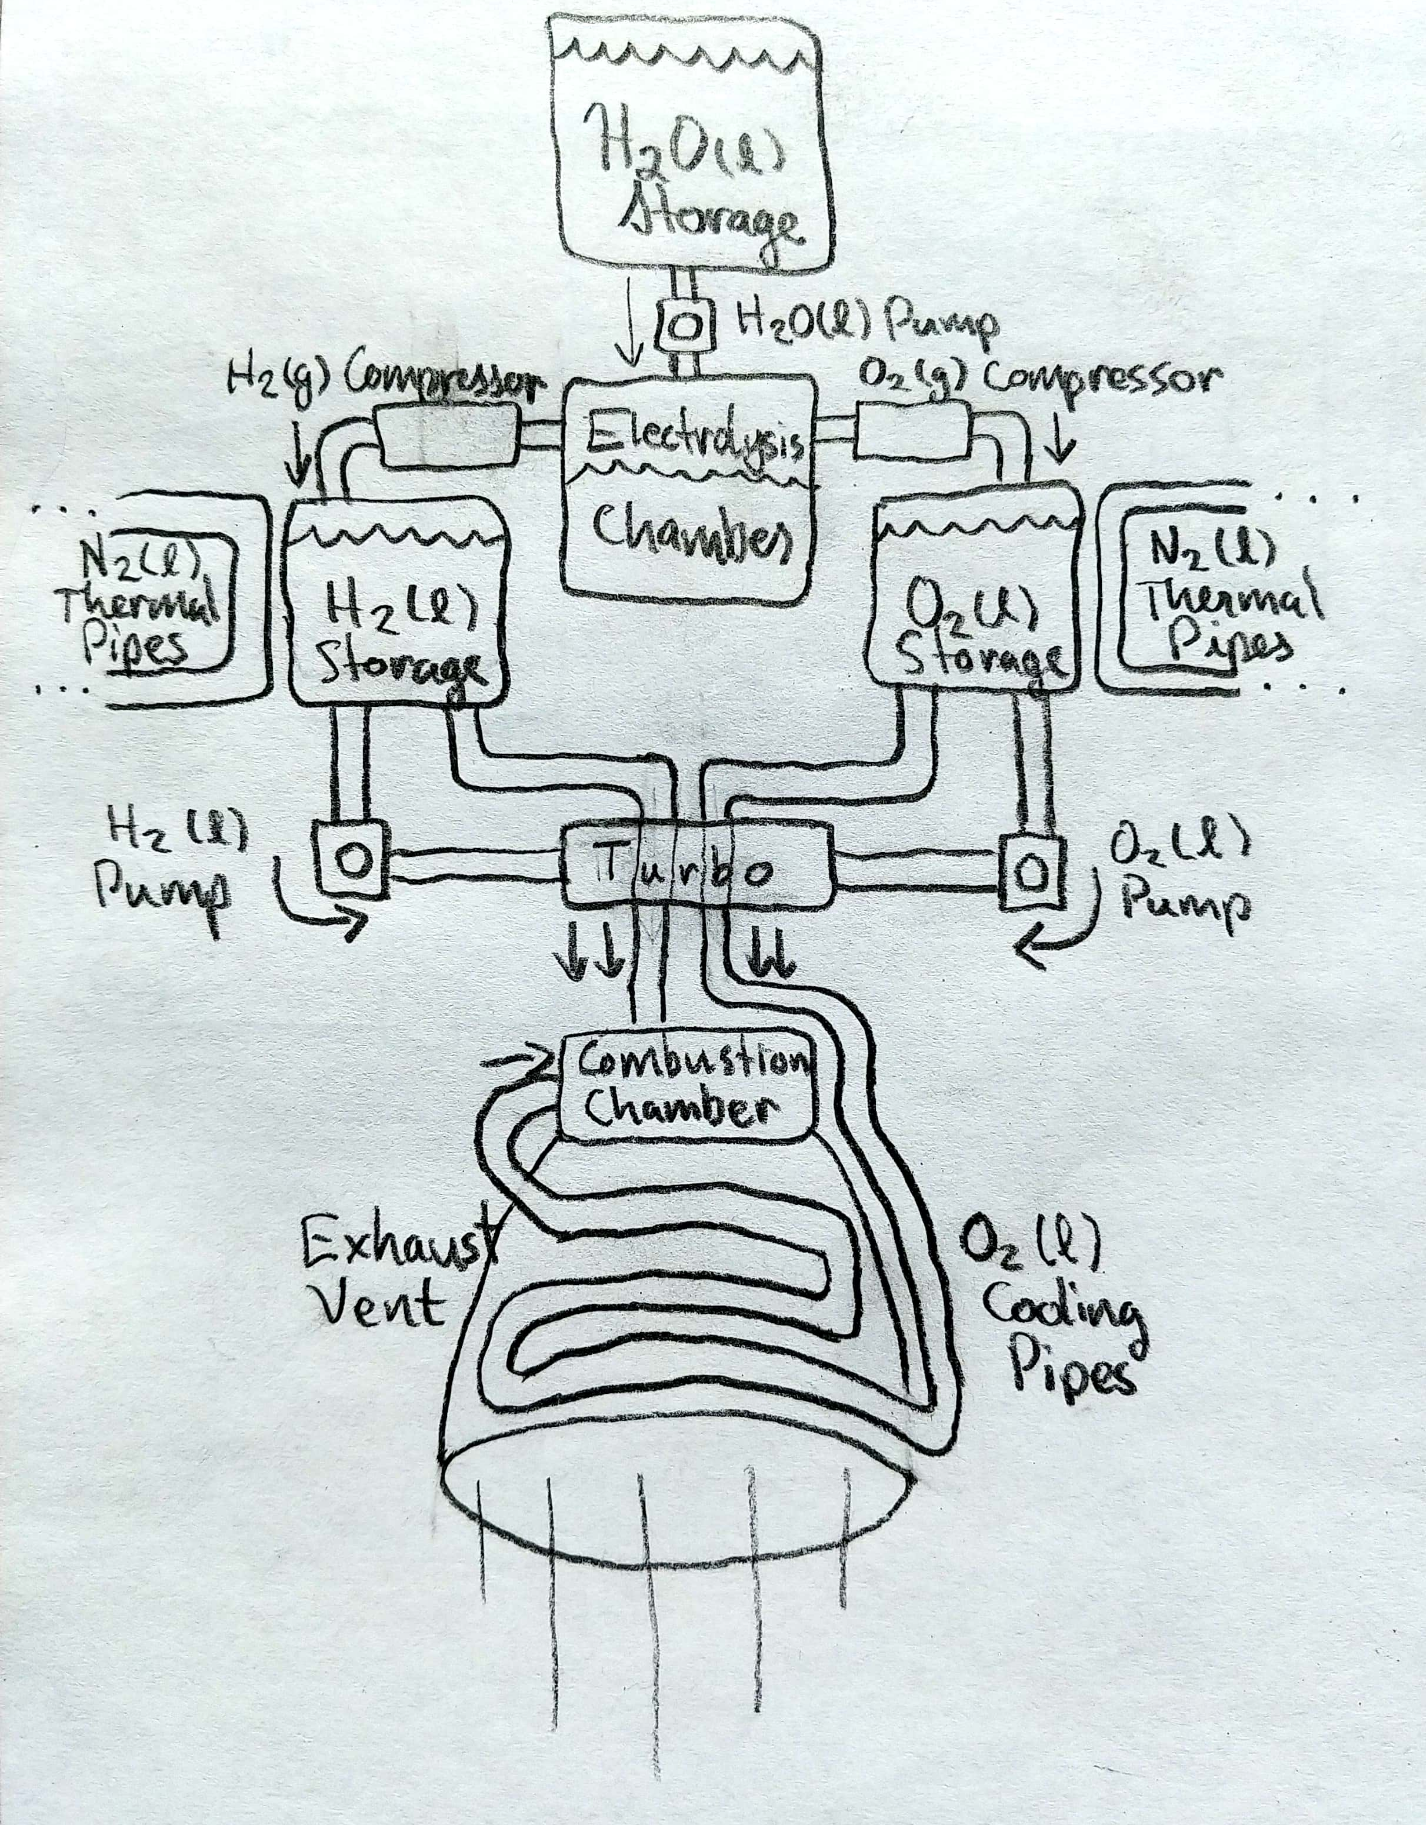
\includegraphics[scale=0.35]{Engine}

\vspace{0.5cm} \hspace{0.25\linewidth}
\begin{tabular}[t]{| c | l | c |}
\toprule
\multicolumn{3}{|l|}{Table \ref{engine} Engine Components} \\
\toprule
1d30 & Component & Link \\
\midrule
1-2 & Electrolysis Chamber & \ref{engine_electrolysis} \\
3 & Turbo & \ref{engine_turbo} \\
4 & Combustion Chamber & \ref{engine_combustion} \\
5-8 & Exhaust Vent & \ref{engine_exhaust} \\
\midrule
9-12 & H$_2$O (l) Storage & \ref{engine_h2o_storage} \\
13 & H$_2$O (l) Pipe & \ref{engine_h2o_pipe} \\
14 & H$_2$O (l) Pump & \ref{engine_h2o_pump} \\
15-16 & H$_2$ (l) Storage & \ref{engine_h2_storage} \\
17-18 & H$_2$ (l) Pipe & \ref{engine_h2_pipe} \\
19 & H$_2$ (g) Condenser & \ref{engine_h2_condenser} \\
20-21 & O$_2$ (l) Storage & \ref{engine_o2_storage} \\
22-23 & O$_2$ (l) Pipe & \ref{engine_o2_pipe} \\
24 & O$_2$ (l) Pump & \ref{engine_o2_pump} \\
25 & O$_2$ (g) Condenser & \ref{engine_o2_condenser} \\
26-29 & O$_2$ (l) Cooling Pipes & \ref{engine_o2_cooling} \\
\bottomrule
\end{tabular}

\vspace{0.3cm}
\begin{minipage}[t]{0.4\linewidth}
Fear
\begin{itemize}
\item The churning of a turbine blade against its casing is a horrific, high-pitched wail which nobody enjoys hearing. See turbo \ref{engine_turbo}, H$_2$O (l) Pump \ref{engine_h2o_pump}, or O$_2$ (l) Pump \ref{engine_o2_pump}.
\end{itemize}
\end{minipage} 
\begin{minipage}[t]{0.4\linewidth}
Anger
\begin{itemize}
\item The flame roaring from a pierced turbo \ref{engine_turbo} or combustion chamber \ref{engine_combustion}, or if a bludgeoning shot rips the seam open. 
\end{itemize}
\end{minipage}

\begin{minipage}[t]{0.4\linewidth}
Isolation
\begin{itemize}
\item When one of the fuel liquids in H$_2$ (l) Storage \ref{engine_h2_storage} or O$_2$ (l) Storage \ref{engine_o2_storage} escapes, it will create a billowing gas. A DM could explore being lost amidst this gas, or use the tension of something it represents. Clouds of hydrogen represent the danger of fire, while clouds of oxygen represent a huge wave of coldness. 
\end{itemize}
\end{minipage}
\begin{minipage}[t]{0.4\linewidth}
Duty
\begin{itemize}
\item When a severely cold liquid escapes, such as in H$_2$ (l) Storage \ref{engine_h2_storage} or O$_2$ (l) Storage \ref{engine_o2_storage}, the whole room will fill with white gas and it will become cold. A true crewman must fix this before things start freezing around him, and so must push directly into the smoke and cold to fix it.
\end{itemize}
\end{minipage}


\hspace{-18pt} \subsubsection{Electrolysis Chamber} \label{engine_electrolysis} \vspace{-0.2cm}
Long-term spacefaring vessels require frequent refueling, meaning most ships elect to use water due to its frequency on planets and in the asteroid belt. Storing hydrogen gas for long periods of time is dangerous, and oxygen is similar, so fuel is stored as liquid water. The liquid water is constantly pumped into the hydrolysis chamber, which uses an electrical current to separate H$_2$O(l) into H$_2$(g) and O$_2$(g). These gases then liquefy in an adjacent condenser, to be stored and used as rocket fuel. Given that a rocket consumes fuel very quickly, this is the main limiting factor in the engine's output, even when the chamber is huge and has many layers of filaments. 

Therefore the engine consists of a large chamber to hold water, a huge number of metal filaments, and escape vents for gas to filter out.
\\ \pbhw
{A small hole is punctured through the casing. \newline \qtwo{A stream of water flows out.}{Either 1d2 H$_2$(g) or O$_2$(g) escapes.}}
{The casing is dented. \newline 1d4 = 1 A seal is broken. Either 1d3 H$_2$O(l), H$_2$(g), or O$_2$(g) escapes.}
{Heats very slowly. \newline 1d4 = 1 An electrical filament overheats. Either 1d2 H$_2$ or O$_2$ production is severely reduced.}
{Filaments must be regularly replaced. Container is subject to acids and oxidation.}


%\begin{enumerate}[label=2cm]
%{A small hole is punctured through the casing. \newline 
%\qtwo{A stream of water flows out.}{Either 1d2 H$_2$(g) or O$_2$(g) escapes.} \\
%{The casing is dented. \newline 1d4 = 1 A seal is broken. Either 1d3 H$_2$O(l), H$_2$(g), or O$_2$(g) escapes.
%{Heats very slowly. \newline 1d4 = 1 An electrical filament overheats. Either 1d2 H$_2$ or O$_2$ production is severely reduced.
%{Filaments must be regularly replaced. Container is subject to acids and oxidation.
%

\vspace{-0.5cm} \hspace{-18pt} \subsubsection{Turbo} \label{engine_turbo} \vspace{-0.2cm}
Given that the engine must stop and let the hydrolysis chamber refuel every now and then, the fuel flow needs to be able to shut off and start up at will. A typical electric motor cannot push enough fuel for an engine to run at full capacity. Instead, a separate stream of rocket fuel is ignited, which then powers the set of main turbines. That is, a separate rocket "engine" is powering the turbines which push fuel into the rocket engine. 

This contraption is called the turbo, which consists of a separate fuel intake powering a miniature combustion chamber, which pushes a drive shaft that connects to the main turbines.
\\ \pbhw
{\qthree{A hole is pierced in the miniature combustion chamber. A small jet of flames escapes when fuel is flowing into the engine, and this fuel flow is slowed slightly.}{A hole is punctured in the blade of either the 1d2 H$_2$ or O$_2$ miniature turbine in the combustion chamber. Its structure is compromised. \newline 1d4 = 1 It shatters when used, and fuel flow is severely reduced until it can be rebalanced.}{A hole is punctured in the blade of either the 1d2 H$_2$ or O$_2$ main turbine. Its structure is compromised. \newline 1d2 = 1 It shatters when used, and fuel flow is severely reduced until it can be rebalanced.}}
{Complete stoppage of flow. Either the 1d2 miniature or main turbine grinds to a halt against its dented outer casing. This is either the 1d2 H$_2$ or O$_2$ turbine.}
{Turbine blade structure weakened. Heats up fuel flowing directly to the exhaust vent cooling system. \newline 1d4 = 1 Turbine blade structure compromised, fuel flow reduced to save it.}
{Turbines require oiling. Over time, exhaust water and oncoming O$_2$ erodes turbine blades. }

\vspace{-0.5cm} \hspace{-18pt} \subsubsection{Combustion Chamber} \label{engine_combustion} \vspace{-0.2cm}
The turbo pumps an enormous amount of liquid oxygen and hydrogen fuel into this chamber, where it is lit, it combusts, and the exhaust escapes out the exhaust vent. 
\\ \pbhw
{Hole pierced in chamber, allowing a huge jet of flame to escape when the engine is firing. Reduces output.}
{Shape of chamber changed, reducing flow and altering exhaust direction vector. \newline 1d4 = 1 Hit so hard that the shape of the output nozzle changes too, significantly limiting exhaust flow. }
{Possible slight structural warping giving similar effects to bludgeoning damage. Otherwise designed to get hot.}
{Severe erosion at nozzle.}


\vspace{-0.5cm} \hspace{-18pt} \subsubsection{Exhaust Vent} \label{engine_exhaust} \vspace{-0.2cm}
Exhaust from the combustion chamber flows out this vent and into space. The particular shape of the vent is designed to maximize the output of the engine. The vent gets very hot, so liquid oxygen fuel is pumped through an extensive array of cooling pipes that surround the vent. This liquid oxygen absorbs much of the heat, and then immediately explodes and flies off to space, taking the heat with it.
\\ \pbhw
{A small hole is pierced through the plate shell of the vent, releasing a jet of hot steam out the side when firing. \newline 1d4 = 1 A structural joint, bolt, or strut is punctured, compromising it. Doing full throttle will result in the structure warping.}
{Structure dented, changed exhaust vector. \newline 1d4 = 1 Structure compromised, so doing full throttle will result in the structure warping.}
{If coolant is flowing, the liquid oxygen can boil before it reaches the combustion chamber, noticeably reducing output. If coolant has stopped, the boiling oxygen will burst the pipes. Afterwards, the heat may begin to warp the engine.}
{Noticeable erosion inside the vent.}



\vspace{-0.5cm} \hspace{-18pt} \subsubsection{H$_2$O (l) Storage} \label{engine_h2o_storage} \vspace{-0.2cm} 
Water is easy to store at room temperature and pressure. However, a zero-gravity ship makes this more complicated. No water tower can provide water pressure, and water in any container will slosh around and mix with the gas in the container. As a result, liquid storage vats contain inflatable bags that hold the liquid itself, while the atmosphere between the bag but still inside the container is pressurized to allow flow and generate water pressure as desired.
\\ \pbhw
{The outside container is punctured. Maintaining pressure becomes difficult, so only passive flow occurs. \newline 1d2 = 1 The inner lining is punctured too. Liquid escapes into the container vat, and passive flow is reduced.}
{The outer container is dented, reducing maximum capacity. If the tank is full, this sends a pressure wave to break the weakest point of the tank, its outflow valve. 1d4 = 1 The outflow valve breaks and water surges out.}
{Water absorbs huge amounts of heat before its temperature rises dangerously. Little effect.}
{Water erodes any container it's in relatively quickly. This is particularly apparent around the input and output valves.}


\vspace{-0.5cm} \hspace{-18pt} \subsubsection{H$_2$O (l) Pipe} \label{engine_h2o_pipe} \vspace{-0.2cm}
It's a pipe with room-temperature, 1 atm pressure water flowing through it. 
\\ \pbhw
{Water flows out.}
{Water flow is reduced.}
{Water absorbs heat easily, so little effect.}
{Water erodes things relatively quickly.}


\vspace{-0.5cm} \hspace{-18pt} \subsubsection{H$_2$O (l) Pump} \label{engine_h2o_pump} \vspace{-0.2cm}
A big fan inside of a pipe. Usually the blades are elongated like a screw.
\\ \pbhw
{Blade structure weakened. 1d4 = 1 Blade shatters, reducing pump flow.}
{Turbine grinds to a halt. 1d4 out of 4 blades are damaged.}
{Blades expand, increasing friction. Blade structure weakens.}
{Requires oiling. }



\vspace{-0.5cm} \hspace{-18pt} \subsubsection{H$_2$ (l) Storage} \label{engine_h2_storage} \vspace{-0.2cm}
Liquid hydrogen is terrifying to store. The liquid can spontaneously evaporate, particularly when jostled or flowing, and it's highly flammable if it hits an oxygen atmosphere. Only so much storage at a time is safe, making this another main limiting factor of the engine. There is no material flexible enough to expand and contract like a bag at such low temperatures, so it is kept in a container that is pressurized highly enough to ensure the majority of the hydrogen inside is liquid.

Liquid hydrogen must be stored below 20 K to ensure no boiling occurs at room pressure \cite{international_temperature_scale_of_1968}. With a pressurized tank, some leniency is given. Expect pressures in the range of tens of atmospheres.
\\ \pbhw
{The huge pressure of the container squirts out a jet of freezing-cold liquid hydrogen. The hydrogen spray would cover the room, immediately evaporating into hydrogen steam. Both the freezing temperature and the evaporation sap heat from the room, quickly making it cold. At the moment of evaporation, the hydrogen gas becomes highly flammable, and the slightest stray spark will completely combust the room, removing all available oxygen and roasting everything inside.}
{The tank is dented. A pressure wave flows throughout the tank. The pressure wave combines with the nucleation site of the dent, both making many bubbles where hydrogen is kicked into evaporating. The pressure wave and the additional pressure from the newly-created gas are likely to overload the opening valve of the tank. \newline 1d2 = 1 The opening valve of the tank bursts, spraying liquid hydrogen throughout the room. The effects will be similar to piercing damage.}
{When liquid hydrogen is heated even slightly, many additional bubbles form from the spontaneous evaporation. \newline 1d2 = 1 The additional bubbles become enough to burst the opening valve of the tank. The effects will be similar to piercing damage.}
{Hydrogen is slightly corrosive, forming rare free radicals that have an acidic effect.}


\vspace{-0.5cm} \hspace{-18pt} \subsubsection{H$_2$ (l) Pipe} \label{engine_h2_pipe} \vspace{-0.2cm}
A highly-insulated strictly-static pipe through which liquid hydrogen flows.
\\ \pbhw
{Liquid hydrogen spills into the room, resulting in smaller but similar effects as piercing damage in \textit{H$_2$ Storage} \ref{engine_h2_storage}.}
{Liquid flow slightly reduced.}
{Hydrogen gas bubbles form and pass the extra pressure on to the next component.}
{Hydrogen is slightly corrosive.}


\vspace{-0.5cm} \hspace{-18pt} \subsubsection{H$_2$ (g) Condenser} \label{engine_h2_condenser} \vspace{-0.2cm}
The liquid hydrogen storage tank is pressurized to ensure its contents are liquid. This has the added benefit that the pressure naturally forces liquid hydrogen out of the container when it is opened, meaning no pump is required. This is helpful since a pump would jostle the liquid hydrogen too much. Still a powerful condenser is needed to put hydrogen into the tank. 

This particular condenser is composed of a chamber which collects hydrogen. This chamber is then mechanically compressed with a piston, increasing the pressure until the hydrogen condenses. Once the pressure is higher than the pressure of the tank, the new liquid hydrogen will freely flow into the tank.
\\ \pbhw
{\qtwo{A hole is pierced behind the piston head, which is harmless as long as the piston stays ahead of it.}{A hole is pierced in front of the piston head, and hydrogen gas will begin to escape. The escapage is especially rapid if the piston is compressing the gas.}}
{\qtwo{A dent is placed behind the piston, stopping it from being able to retract fully.}{A dent is placed in front of the piston, stopping it from being able to compress fully.}}
{The dangerous part is the hydrogen absorbing the heat, which then is transferred directly into the hydrogen storage.}
{Pistons require lubrication and maintenance.}


\vspace{-0.5cm} \hspace{-18pt} \subsubsection{O$_2$ (l) Storage} \label{engine_o2_storage} \vspace{-0.2cm}
The oxygen storage tank is similarly supercooled to around 60 K and pressurized to a handful of tens of atmospheres. Oxygen is slightly more forgiving, since it won't explode or spontaneously boil, though it's highly corrosive to the wrong materials.
\\ \pbhw
{A stream of highly pressurized liquid oxygen at unbelievably cold temperatures streams outward and covers the room. The oxygen sucks heat out of the air both to warm itself up and to boil away, leaving everything a frost-covered mess. A high concentration of oxygen in the room allows for many more things to burn than normal, and at even lower temperatures, making the risk of fires high.}
{The tank is dented, sending a sudden pressure wave to the output valve. \newline 1d4 = 1 The pressure is enough to burst the output valve, and oxygen floods out. The effects will be similar to piercing damage.}
{Liquid oxygen will boil if its temperature gets too high, though not as sensitively as hydrogen. \newline 1d4 = 1 The boiling creates enough additional pressure to burst the output valve, and oxygen floods out. The effects will be similar to piercing damage.}
{Oxygen corrodes the wrong materials, though the tank is designed to avoid that. }


\vspace{-0.5cm} \hspace{-18pt} \subsubsection{O$_2$ (l) Pipe} \label{engine_o2_pipe} \vspace{-0.2cm}
This pipe carries liquid oxygen from place to place. 
\\ \pbhw
{Liquid oxygen leaks out. Use a less dangerous version of the piercing damage section of \textit{O$_2$(l) Storage} \ref{engine_o2_storage}}
{Limits liquid flow rate.}
{Transfers heat to downstream component.}
{Designed to withstand oxygen corrosion.}


\vspace{-0.5cm} \hspace{-18pt} \subsubsection{O$_2$ (l) Cooling Pipes} \label{engine_o2_cooling} \vspace{-0.2cm}
Since oxygen has a decent specific heat capacity, these pipes wrap around the exhaust vent several times. Otherwise these pipes are identical to the above O$_2$(l) pipes.

\vspace{-0.5cm} \hspace{-18pt} \subsubsection{O$_2$ (l) Pump} \label{engine_o2_pump} \vspace{-0.2cm}
While a decent flow comes out of the liquid oxygen storage tank due to the pressurization of the liquid, it's not enough to push the liquid around the exhaust vent several times. An additional liquid pump is required, which is simply a small turbine that pushes the liquid through it.
\\ \pbhw
{A turbine blade has a hole punched through it, compromising its structure. \newline 1d4 = 1 It shatters when used, stopping its addition to the flow until it can be rebalanced.}
{The turbine grinds to a halt. 1d4 of the 4 turbine blades are damaged.}
{Heating here will transfer to the exhaust vent.}
{Designed to withstand oxygen corrosion.}


\vspace{-0.5cm} \hspace{-18pt} \subsubsection{O$_2$ (g) Condenser} \label{engine_o2_condenser} \vspace{-0.2cm}
An oxygen condenser is similar to a hydrogen condenser except that it's significantly safer.
\\ \pbhw
{\qtwo{A hole is pierced behind the piston head, which is harmless as long as the piston stays ahead of it.}{A hole is pierced in front of the piston head, and oxygen gas will begin to escape. The escapage is especially rapid if the piston is compressing the gas.}}
{\qtwo{A dent is placed behind the piston, stopping it from being able to retract fully.}{A dent is placed in front of the piston, stopping it from being able to compress fully.}}
{Oxygen will absorb the heat readily, though it will heat up relatively slowly, and this will be transferred into the oxygen storage.}
{Pistons require lubrication and maintenance.}

\newpage
\subsection{Thermal} \label{thermal}

Every ship in space generates heat via various mechanisms. Any energy generation has some inefficiency which becomes stray heat, weaponry creates heat on firing, and every other system generates at least some heat as well. If a spaceship were left in space with no way to get rid of its heat, it would melt far more quickly than it would freeze. As a result, every ship is equipped with a thermal system, a system designed to take the heat from all the other parts of the ship and to get rid of it.

Most systems aboard a ship operate at room temperature. For these systems, liquid water works perfectly fine as a conduit to transfer heat to the radiator. Even systems that generate large amounts of heat like weaponry can be handled by water due to its specific heat capacity. However, certain parts of the ship require extreme temperatures. The radiator must be excruciatingly hot, while liquid fuel for the engines and liquid helium in magnetic field coils must be near absolute zero. For these, a compressible substance is needed. Compressible substances can be compressed and expanded at will, unlike water, allowing their temperature to be varied as needed.

If the radiator or nitrogen circuit stops, heat will continue being transferred into the heat sink until the heat sink becomes full. When the heat sink is full, heat can be dumped into any system that can handle it. If the water circuit stops, heat will start to be generated by every system on the ship. Each system will simultaneously have to fight off heat-related problems, though more severe for systems that generate lots of heat like weaponry.

\vspace{0.2cm}
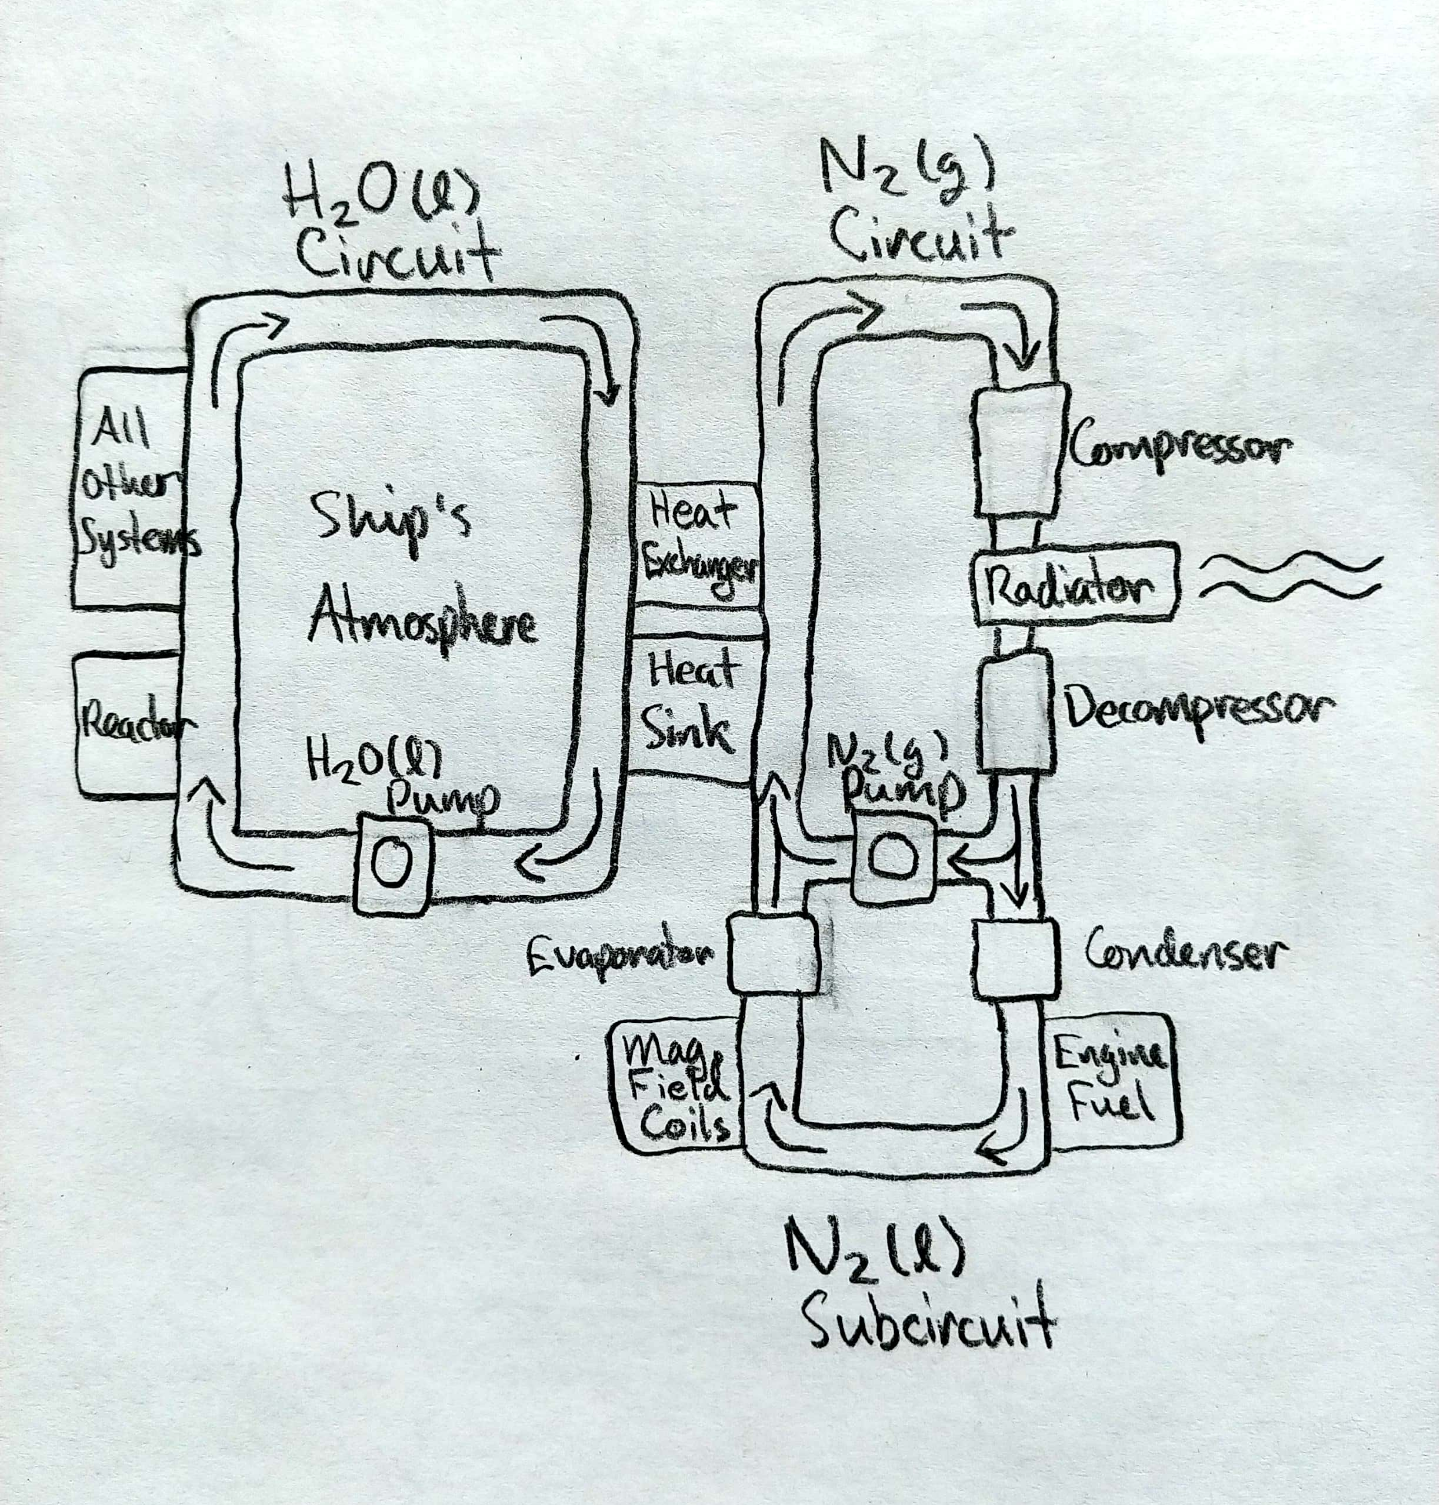
\includegraphics[scale=0.275]{Thermal}

\vspace{0.5cm} \hspace{0.25\linewidth}
\begin{tabular}{| c | l | c |}
\toprule
\multicolumn{3}{|l|}{Table \ref{thermal} Thermal Components} \\
\toprule
1d10 & Component & Link \\
\midrule
1 & Radiator & \ref{thermal_radiator} \\
2 & Compressor & \ref{thermal_compressor} \\
3 & Heat Exchanger & \ref{thermal_exchanger} \\
4 & Heat Sink & \ref{thermal_sink} \\
\midrule
5-6 & H$_2$O (l) Pipe & \ref{thermal_h2o_pipe} \\
7 & H$_2$O (l) Pump & \ref{thermal_h2o_pump} \\
8-9 & N$_2$ (g) Pipe & \ref{thermal_n2_pipe} \\
10 & N$_2$ (g) Pump & \ref{thermal_n2_pump} \\
\bottomrule
\end{tabular}

\vspace{0.3cm}
\begin{minipage}[t]{0.4\linewidth}
Fear
\begin{itemize}
\item If a single hole were poked into the radiator \ref{thermal_radiator}, or if a bludgeoning attack tears a crack in it, a laser beam of heat would escape. This beam would be raging hot, something that nobody should touch, nobody should see. The belly of the beast is a raw and powerful thing.
\end{itemize}
\end{minipage} 
\begin{minipage}[t]{0.4\linewidth}
Anger
\begin{itemize}
\item Heat is often synonymous with anger. If a player is getting particularly angry, consider having the thermal pipes that carry water to their system H$_2$O (l) Pipe \ref{thermal_h2o_pipe} burst. This way their machine will become hot to be around, hot to the touch, and further problems may arise. 
\end{itemize}
\end{minipage}

\begin{minipage}[t]{0.4\linewidth}
Isolation
\begin{itemize}
\item Something small and insignificant stops working, like a compressor \ref{thermal_compressor}. Perhaps even a simple fix. However, for a brief moment, the radiator must stop running, and heat must build up. The ship is only one tiny malfunction away from the radiator completely stopping, and the ship would boil alive. The only line of defense that the ship has is the player.
\end{itemize}
\end{minipage}
\begin{minipage}[t]{0.4\linewidth}
Duty
\begin{itemize}
\item When a radiator \ref{thermal_radiator} breaks open, the air around it becomes singed with heat and plasma, and the walls of the room facing the opening grow red hot. If more heat keeps spilling into the room, it will overheat the enginery and overload the atmosphere's climate control. The lone player must venture directly toward the radiator, into the blazing heat and sizzling air, and have the courage to place something over the breakage to stop it.
\end{itemize}
\end{minipage}

\hspace{-18pt} \subsubsection{Radiator} \label{thermal_radiator} \vspace{-0.2cm}

The radiator is the component that actually sends heat flying away. All objects constantly release some energy in the form of light as a result of their temperature. Hotter objects like the sun release more energy as light. Larger objects also release more energy, which is why the ISS is equipped with huge arrays of white panel radiators.

Aboard a combat vessel, a ship's radiator should be as small as possible to avoid being damaged. As a result, high-temperature radiators are used. These radiators dump waste heat into an extremely hot metal filament. The insane temperature of the filament means that it will radiate heat much more quickly. The waste heat therefore escapes out the radiator and is reflected into a thin cone pointed in a single direction.
\\ \pbhw
{A hole is pierced through the casing of the radiator. The heat from the radiator escapes through this hole. The air begins to noticeably warm, and wherever the beam of heat is shining becomes red-hot quickly. \newline 1d4 = 1 The shot pierces through the filament as well. Sudden kicks to the ship or full-throttle acceleration may cause the filament to snap. If it snaps, the tip of the filament will touch the casing at a single point, beginning to melt it.}
{The casing of the radiator is dented, altering its outflow direction slightly. \newline 1d2 = 1 The denting is enough to touch the filament. The casing at that point immediately becomes red hot and will quickly melt.}
{The radiator is designed to get stupidly hot.}
{The filament needs to be changed regularly.} 


\vspace{-0.5cm} \hspace{-18pt} \subsubsection{Compressor} \label{thermal_compressor} \vspace{-0.2cm}
Just before nitrogen enters the radiator to transfer its heat to the filament, the nitrogen must become hotter than the filament. This work is done by a compressor, squeezing the gas by so much that its temperature rises significantly. Once it has transferred its heat, a decompresser just after the nitrogen leaves the radiator will return it to normal pressure levels.
\\ \pbhw
{\qtwo{The piercing shot hits the compressor while nitrogen is still highly pressurized. A stream of piping-hot nitrogen shoots out of the pipage.}{The piercing shot hits the while nitrogen is depressurized. A small leakage of nitrogen gas escapes.}}
{\qtwo{The dent prevents the compressor from fully compressing the gas.}{The dent prevents the compressor from fully entering the decompressed state.}}
{The nitrogen takes the heat and dumps it directly into the radiator.}
{Compressors require oiling and are subject to mechanical erosion.}


\vspace{-0.5cm} \hspace{-18pt} \subsubsection{Heat Exchanger} \label{thermal_exchanger} \vspace{-0.2cm}
The thermal system on large ships is split into two separate circuits: the main H$_2$O (l) circuit which cools the majority of systems, and the secondary N$_2$ (g) circuit which cools the very cold systems and heats the very hot ones. Between these two systems is an interface called the heat exchanger. This exchanger keeps the two liquids separate, but separates them by a material that allows heat to pass easily. This means that the waste heat in the water circuit can be constantly passed to the nitrogen circuit in order to release it out the radiator.

The exchanger separates water and nitrogen into large sheets and lets them flow down either side of a large boundary. Several layers of sheets are included to increase the total heat flow rate.
\\ \pbhw
{\qeq{1d4}{1.}{The shot hits both a water tube and a nitrogen tube, releasing both a stream of water and a cloud of gas.}{2.}{The shot hits a nitrogen tube, releasing nitrogen gas into the atmosphere.}{3.}{The shot hits a water tube, and lukewarm water sprays out.}{4.}{The shot misses everything.}}
%{Flip two coins. \newline \qtwo{The shot misses any water tube.}{The shot hits a water tube, and lukewarm water sprays out.}  \qtwo{The shot misses any nitrogen tube.}{The shot hits a nitrogen tube, releasing it.}}
{The dent will certainly cause flow to slow somewhere. However, there are so many different tubes and panels that it will go mostly unnoticed.}
{The exchanger will dump heat into the nitrogen.}
{The exchanger is subject to erosion on both sides across a huge surface area. Layers require frequent cleaning and replacing.}


\vspace{-0.5cm} \hspace{-18pt} \subsubsection{Heat Sink} \label{thermal_sink} \vspace{-0.2cm}
When the radiator needs repairs, or when too much heat is entering the ship for the radiator to handle, the extra heat can be dumped into a heat sink. In the majority of cases this heat sink is the engine's water fuel tank, since water has an impressive specific heat capacity and a lot of water is carried in the tank. For problems with this tank, see \textit{H$_2$O (l) Storage} \ref{engine_h2o_storage}. When nearly empty, certain metal parts of the hull can also absorb much heat. 

\vspace{-0.5cm} \hspace{-18pt} \subsubsection{H$_2$O (l) Pipe} \label{thermal_h2o_pipe} \vspace{-0.2cm}
It carries water. Amazing.
\\ \pbhw
{Water spills out.}
{Water flow is slowed.}
{The water carries heat to the heat exchanger.}
{Water erodes pipes relatively quickly compared to other liquids.}


\vspace{-0.5cm} \hspace{-18pt} \subsubsection{H$_2$O (l) Pump} \label{thermal_h2o_pump} \vspace{-0.2cm}
A water pump is a big wet fan.
\\ \pbhw
{The structure of a fan blade becomes compromised. \newline 1d4 = 1 The blade shatters, severely slowing flow until it can be rebalanced.}
{The fan grinds to a halt. A total of 1d4 out of the 8 blades are damaged.}
{The fan is cooled by the water around it.}
{Water erodes fans quickly.}


\vspace{-0.5cm} \hspace{-18pt} \subsubsection{N$_2$ (g) Pipe} \label{thermal_n2_pipe} \vspace{-0.2cm}
A pipe that holds nitrogen. When these pipes carry nitrogen to a system that requires extreme cooling, the nitrogen passes through a condenser first to be turned into a liquid. This allows it to reach temperatures far lower than as a gas. Afterwards it is turned back into a gas via an evaporator and the nitrogen rejoins the gas circuit.
\\ \pbhw
{Nitrogen gas spills out.  }
{The flow of nitrogen gas is limited slightly.}
{The nitrogen delivers its heat directly to the radiator. If the nitrogen is in liquid form, extra heat may cause some to boil. This is not dangerous in small quantities, since the evaporator handles gases just fine. In large quantities, bursting may occur from the unexpected pressure increase.}
{Little wear or tear.}


\vspace{-0.5cm} \hspace{-18pt} \subsubsection{N$_2$ (g) Pump} \label{thermal_n2_pump} \vspace{-0.2cm}
A pump that pushes gaseous nitrogen through its circuit. It is literally just a fan.
\\ \pbhw
{One of the blades is punctured. \newline 1d4 = 1 The blade shatters on use, severely slowing nitrogen flow until it can be rebalanced.}
{The blades grind to a halt against their casing. A total of 1d4 out of 4 of the blades are damaged.}
{The pump is cooled by the nitrogen.}
{Little wear or tear.}


\newpage
\subsection{Railgun} \label{railgun}

A railgun is composed of two parallel metal rails with a round of ammunition, a small hunk of metal flak, sandwiched between them. Huge amounts of current is passed through this system, traveling down one rail, through the metal flak, and then back the other rail. The particular circular movement of current generates a magnetic field, and individual electrons in the current through the flak round experience a force as a result of the moving through the magnetic field. With a capacitor to store a huge amount of electrical energy and a switch to release it, the large voltage from the capacitor will draw a large current from the electrical grid. The will generate an enormous force on the small flak round. Railguns can typically accelerate a small round to velocities at least 2.5 km/s \cite{naval_railgun} and up to 5.9 km/s \cite{scientific_railgun}.

\vspace{0.2cm}
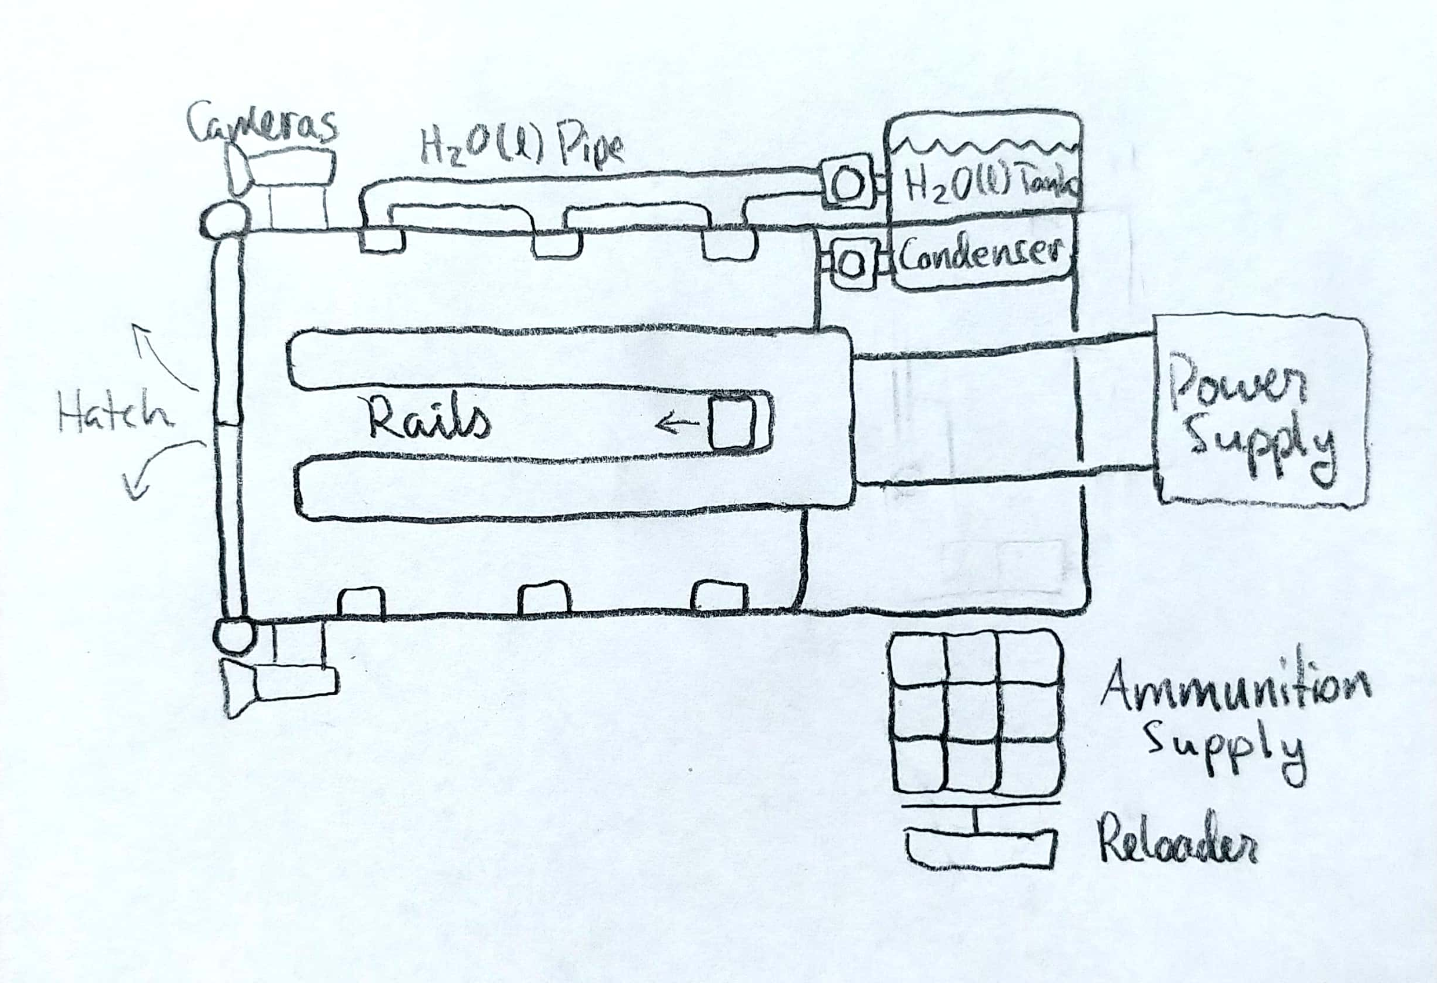
\includegraphics[scale=0.275]{Railgun}

\vspace{0.5cm} \hspace{0.25\linewidth}
\begin{tabular}{@{} | c | l | c | @{}}
\toprule
\multicolumn{3}{|l|}{Table \ref{railgun} Railgun Components} \\
\toprule
1d20 & Component & Link \\
\midrule
1-4 & Rails & \ref{railgun_rails} \\
5 & Reloader & \ref{railgun_reloader} \\
6-7 & Hatch & \ref{railgun_hatch} \\
8 & Cameras & \ref{railgun_cameras} \\
9-12 & Ammunition Supply & \ref{railgun_ammunition} \\
\midrule
13 & H$_2$O (g) Condenser & \ref{railgun_h2o_condenser} \\
14 & H$_2$O (g) Pump & \ref{railgun_h2o_g_pump} \\
15-17 & H$_2$O (l) Pipe & \ref{railgun_h2o_pipe} \\
18 & H$_2$O (l) Pump & \ref{railgun_h2o_l_pump} \\
\bottomrule
\end{tabular}

\vspace{0.3cm}
\begin{minipage}[t]{0.4\linewidth}
Fear
\begin{itemize}
\item The railgun can get messy. Consider first having the ammunition supply \ref{railgun_ammunition} get bludgeoned so that the room is covered with floating metal cubes getting in the way of everything. Also make sure to emphasize the sound of the railgun itself as it fires: the scrape of metal on metal, the hiss of gases and water sizzling, and the hum of pumps and pistons resetting the gun.
\end{itemize}
\end{minipage} 
\begin{minipage}[t]{0.4\linewidth}
Anger
\begin{itemize}
\item If a breakage causes the thermal system of the railgun to temporarily stop, it can still theoretically be fired. Pushing it like this will heat the rails up to huge temperatures, and could parallel a character's recklessness well.
\end{itemize}
\end{minipage}

\begin{minipage}[t]{0.4\linewidth}
Isolation
\begin{itemize}
\item Gazing through the cameras \ref{railgun_cameras} shows complete darkness most of the time, and otherwise only shows the smallest red blip of another ship. The gunner has the closest connection to space outside, so make sure there's a window nearby. Occasionally describe their shots disappearing into the void when they miss.
\end{itemize}
\end{minipage}
\begin{minipage}[t]{0.4\linewidth}
Duty
\begin{itemize}
\item A railgun that's lost its cameras \ref{railgun_cameras} or its computer system can still be aimed and fired manually. Perhaps a player must fire the last critical shot at an enemy by hand. 
\end{itemize}
\end{minipage}

\hspace{-18pt} \subsubsection{Rails} \label{railgun_rails} \vspace{-0.2cm}
Two long metal rails are precisely engineered to be smooth and an exact distance away from each other, so that they fit rounds of ammunition snugly. Unfortunately no matter the smoothness, the railgun still loses much energy to friction and to the partial deformation of the rails. The friction generates huge amounts of heat, so a railgun can only fire one shot before requiring cooling. It is cooled by sealing the railgun with exterior flaps, pumping the chamber full of atmosphere and then spraying the rails with water via sprinklers, which evaporates and sucks heat away.  
\\ \pbhw
{The structure of one of the rails is compromised. The outer casing is pierced, so a small amount of atmosphere and water escapes each cooling cycle. \newline \hspace{-3pt} The next time the railgun is fired, the railgun shot will warp the rail enough to break the flow of current between them, weakening the shot until the rail is changed. A rapid change from hot to cold or vice-versa via the heating system could also cause such a significant warpage.}
{The outer casing of the railgun is hugely dented, and the rail took the brunt of the rest of the hit. It is deformed enough to break the flow of current halfway through the shot, weakening the shot and making it much less accurate until the rail is changed.}
{Heating will weaken the metal just like firing a shot.}
{The frequent heating and cooling of the rails weakens the metal and can contribute to developing cracks, and the flak scrapes metal away as it is fired and this can deform the rails further. This means that rails need to be frequently changed out even under optimal conditions.}


\vspace{-0.5cm} \hspace{-18pt} \subsubsection{Reloader} \label{railgun_reloader} \vspace{-0.2cm}
The railgun fires several shots at a time, cooling between each one, before returning to upright position to reload. The reloading mechanism is a simple piston which pushes a chunk of cubical metal slugs into the railgun, while maintaining a seal. This device is typically broken when directly being used, so when the piston is expanding and retracting.
\\ \pbhw
{\qtwo{The piston arm or head is pierced, weakening it though not noticeably.}{The piston's pneumatics are pierced, releasing water and immediately shrinking the bottom of the piston arm down to the level of the hole.}}
{\qtwo{The piston arm is dented, and will not push straight nor far enough.}{The pneumatic cylinder is dented, preventing the bottom of the piston arm from dropping lower than the dent.}}
{The piston head is a relatively small piece of metal, meaning it can heat up quickly.}
{Pistons require lubrication and occasional maintenance.}


\vspace{-0.5cm} \hspace{-18pt} \subsubsection{Hatch} \label{railgun_hatch} \vspace{-0.2cm}
The entire railgun arms are enclosed in a cylindrical casing. At the muzzle, a hatch opens so that the railgun can fire into the vacuum of space. 
\\ \pbhw
{Some water and atmosphere escape when cooling the railgun.}
{\qtwo{The hatch is stuck open.}{The hatch is stuck closed.}}
{The hatch becomes much easier to push open from the inside.}
{The hatch requires lubrication and decays under stellar radiation.}


\vspace{-0.5cm} \hspace{-18pt} \subsubsection{Cameras} \label{railgun_cameras} \vspace{-0.2cm}
A railgun is equipped with several thermal cameras which track the locations of enemy ships so that targeting computers can properly aim the railguns. There are at least two cameras per railgun in order to help estimate distances.
\\ \pbhw
{\qtwo{A part of the electronics of the camera is pierced through, completely disabling it.}{The lens chamber is pierced, allowing in extra light.}}
{One of the cameras is smashed to pieces.}
{The intricate electronics of a camera's optical sensor will be the first to melt, followed by the rest of the circuitry.}
{Cameras in space are subject to harmful radiation. Stray UV photons fry individual pixels of the optical sensor over time. Those same photons can interfere with wiring as well and cause errors in the electronics of the camera. Cameras have some shielding but this is still not enough.}


\vspace{-0.5cm} \hspace{-18pt} \subsubsection{Ammunition Supply} \label{railgun_ammunition} \vspace{-0.2cm}
Somewhere next to the railgun a huge pile of ammunition is stored. This is just a cube of stacked metal slugs, where each slug is a cube as well, with a piston to push slugs into reloading position.
\\ \pbhw
{A total of 1d4 slugs now have a hole in them.}
{A total of 1d4 slugs are smashed into unusable shape and another 1d12 slugs go flying off into the room.}
{The metal slugs can absorb a ton of heat.}
{Slugs need to have precisely manufactured dimensions in order to fit between the perfect distance between the rails. Deforming them in any way will most of the time make them unusable.}


\vspace{-0.5cm} \hspace{-18pt} \subsubsection{H$_2$O (g) Condenser} \label{railgun_h2o_condenser} \vspace{-0.2cm}
Spraying water into the railgun chamber utilizes the huge amount of latent heat required to turn water from liquid into steam. The steam is vented out by a steam pump, and needs to be recovered. Thermal pipes curl around several times to provide ample surface area for water to condense, drip, and be collected for spraying again.
\\ \pbhw
{Some steam escapes. \newline 1d2 = 1 A thermal pipe is also pierced. Additional water flows into the condenser until it can be plugged.}
{The condenser chamber is dented. \newline 1d4 = 1 The denting is enough to break a seal somewhere, and steam escapes.}
{If this component ends up collecting extra heat, it will increase the temperature difference between steam and thermal pipe and therefore will increase the heat flow rate into from the steam into the pipe. Thus the steam will condense even faster.}
{Water will corrode both sides of the thermal pipes, making them subject to annual replacement.}


\vspace{-0.5cm} \hspace{-18pt} \subsubsection{H$_2$O (g) Pump} \label{railgun_h2o_g_pump} \vspace{-0.2cm}
It's a big fan.
\\ \pbhw
{One of the turbine blades has a hole pierced through it. \newline 1d4 = 1 The hole is enough to shatter the blade when it starts spinning too quickly. }
{The turbine comes screeching to a halt. A total of 1d4 out of 8 blades are damaged.}
{The turbine will transfer heat to the steam. }
{The turbine erodes moderately quickly due to the steam.}


\vspace{-0.5cm} \hspace{-18pt} \subsubsection{H$_2$O (l) Pipe} \label{railgun_h2o_pipe} \vspace{-0.2cm}
It's a pipe that carries water.
\\ \pbhw
{Water spills out.}
{Limits water flow slightly.}
{Transfers heat to the railgun when sprayed on it.}
{Water wears pipes decently quickly.}


\vspace{-0.5cm} \hspace{-18pt} \subsubsection{H$_2$O (l) Pump} \label{railgun_h2o_l_pump} \vspace{-0.2cm}
It's literally just a big wet fan.
\\ \pbhw
{One of the turbine blades has a hole pierced through it. \newline 1d4 = 1 The hole is enough to shatter the blade when it starts spinning too quickly. }
{The turbine comes screeching to a halt. A total of 1d4 out of 8 blades are damaged.}
{The turbine will transfer heat to the water.} 
{The turbine erodes quickly from the water.}


\newpage
\subsection{Ray Accelerator} \label{ray}

The ray accelerator is a theoretical weapon based on the particle accelerators of modern day. The machine ionizes a material, accelerates it by spinning it around a circular path, and then lets the stream of hot ionized gas fly toward the enemy. While no proper experiments have been done to determine this, it is likely that the shot will penetrate through essentially anything it comes across due to the pinpoint accuracy available when using voltages for precise targeting \cite{energy_weapons}.

\vspace{0.2cm}
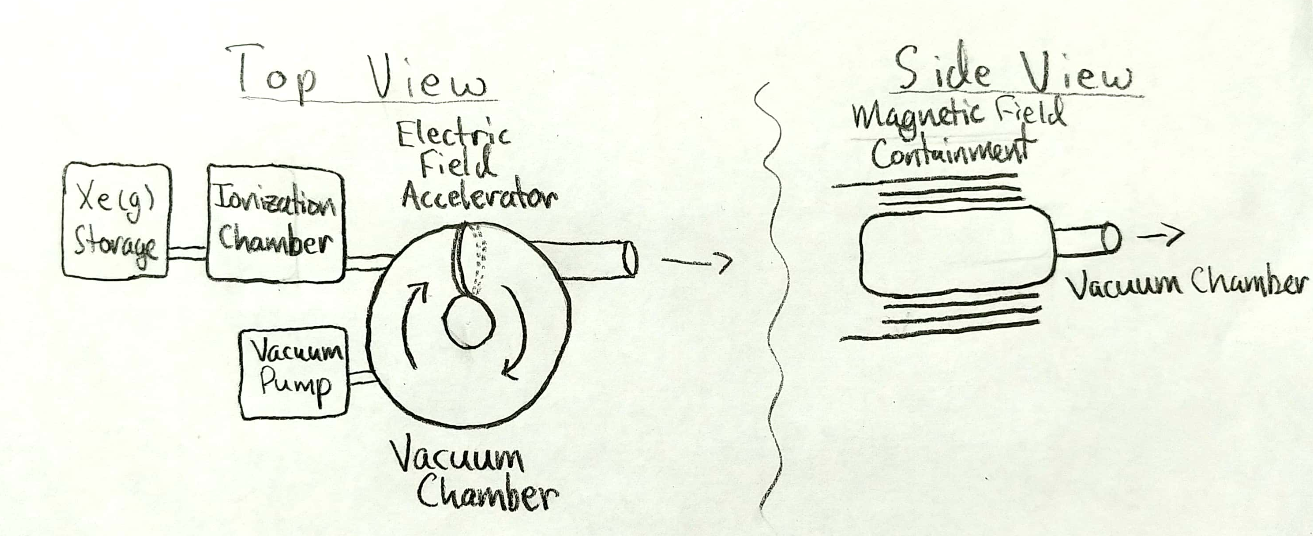
\includegraphics[scale=0.3]{Ray_Accelerator}

\vspace{0.5cm} \hspace{0.25\linewidth}
\begin{tabular}{@{} | c | l | c | @{}}
\toprule
\multicolumn{3}{|l|}{Table \ref{ray} Ray Components} \\
\toprule
1d10 & Component & Link \\
\midrule
1-4 & Vacuum Chamber & \ref{ray_chamber} \\
5 & Ionization Chamber & \ref{ray_ionization} \\
6 & Electric Field Accelerator & \ref{ray_accelerator} \\
7-8 & Magnetic Field Containment & \ref{ray_containment} \\
9 & Xe (g) Storage & \ref{ray_xe_storage} \\
10 & Vacuum Pump & \ref{ray_vacuum_pump} \\
\bottomrule
\end{tabular}

\vspace{0.3cm}
\begin{minipage}[t]{0.4\linewidth}
Fear
\begin{itemize}
\item The xenon is spinning right there in the main vacuum chamber \ref{ray_chamber}, mere feet away from the gunner. If a container magnet \ref{ray_containment} so much as malfunctions slightly, that beam of xenon will pierce through the walls of its chamber just as easily as an enemy. 
\end{itemize}
\end{minipage} 
\begin{minipage}[t]{0.4\linewidth}
Anger
\begin{itemize}
\item The vacuum can fail in the main chamber \ref{ray_chamber} or the ionization chamber \ref{ray_ionization}, and once it fails it takes a long time to reestablish the full vacuum. I could see a character's frustration building as they cannot seem to get a vacuum to stay put, taking up long amounts of time where the ray is completely inoperable.
\end{itemize}
\end{minipage}

\begin{minipage}[t]{0.4\linewidth}
Isolation
\begin{itemize}
\item If all the xenon gas in its storage \ref{ray_xe_storage} escapes, which is surprisingly likely, there's no backup xenon anywhere. The player must come up with something themselves that can be used in place of xenon and scavenge it from a different part of the ship. Make sure the captain or another crew asks for frequent updates on the ray.
\end{itemize}
\end{minipage}
\begin{minipage}[t]{0.4\linewidth}
Duty
\begin{itemize}
\item The electromagnets (in \ref{ray_accelerator} and \ref{ray_containment}) are finely positioned and critical to the system. If something knocks them out of place, the whole system fails. A particularly heroic crew member might need to stand up on top of the vacuum chamber and use their strength to force a hot metal coil back into place while it sizzles and sparks in their hands.
\end{itemize}
\end{minipage}

\hspace{-18pt} \subsubsection{Vacuum Chamber} \label{ray_chamber} \vspace{-0.2cm}
The gaseous material needs to be accelerated to incredible speeds in order for such otherwise weak gases to deal damage. This simply is not possible in an atmosphere, since air resistance will completely destroy such small quantities of gas. Therefore the donut in which the gas is accelerated has a near-perfect vacuum maintained in it.
\\ \pbhw
{The vacuum quickly weakens to unacceptable levels and the gas becomes unable to accelerate.}
{The chamber is dented. \newline 1d2 = 1. The dent is enough to break the vacuum seal, quickly destroying the vacuum. \newline 1d2 = 1. The dent is enough to get in the way of the beam of gas as it accelerates, meaning the ray cannot fire until this dent is undone.}
{The metal walls of the chamber can store a decent amount of heat, though they do not get rid of it very quickly.}
{A vacuum is never perfect and the seal weakens over time. }


\vspace{-0.5cm} \hspace{-18pt} \subsubsection{Ionization Chamber} \label{ray_ionization} \vspace{-0.2cm}
Only charged particles are affected by electric and magnetic field, meaning the gas needs to be ionized before use. A shot's worth of gas is sprayed into the ionization chamber, where it is bombarded with electrons until electrons are knocked off. Like the acceleration chamber, this chamber must be at a vacuum as well.
\\ \pbhw
{The vacuum is destroyed, xenon gas leaks out, and stray electrons can leak out.}
{The chamber is dented. \newline 1d2 = 1. The dent is enough to break the seal, destroying the vacuum.}
{The chamber walls will heat up and stay hot.}
{Vacuum seal weakens over time. Inside walls become damaged by ions and bombardment.}


\vspace{-0.5cm} \hspace{-18pt} \subsubsection{Electric Field Accelerator} \label{ray_accelerator} \vspace{-0.2cm}
Each time that the gas goes around in a circle inside the main vacuum chamber, it passes the accelerator. This device generates a strong electric field that will accelerate charged particles that pass through it in the proper direction. If it circles enough times, its velocity will eventually be so large that the gas can pierce nearly anything.

This particular design of electric field uses an electromagnet wrapped around a single slice of the main vacuum chamber. Energy is dumped rapidly into the magnet coil, and the rapid rise in a magnetic field can generate a strong electric field as well. As long as the timings for when the particles arrive at the accelerator and when the magnetic field is increasing or decreasing are matched up, this can accelerate particles to huge velocities.
\\ \pbhw
{The wiring of the electromagnet is pierced. The casing is open, meaning sparks can fly. \newline 1d2 = 1. The piercing completely nicks the wiring, stopping all electrical flow.}
{The electromagnet is bent out of shape, altering the precise direction that it accelerates the particles in the main chamber. As a result the beam of particles will eventually hit the wall, and the weapon cannot accelerate its shot to proper speed.}
{The wiring will warp and can come in contact with the vacuum chamber. Even slight warping will alter the direction of acceleration, scattering the beam far before it can fire every time it is shot.}
{Such swings in current will wear even a strong wire decently quickly.}


\vspace{-0.5cm} \hspace{-18pt} \subsubsection{Magnetic Field Containment} \label{ray_containment} \vspace{-0.2cm}
The particles inside the vacuum chamber need some force that keeps them spinning in a circle. This force is conveniently supplied just by placing strong magnets above and below. The faster the particle is moving, the stronger the magnetic field needs to be, so its power increases over time as a shot is fired.

The magnetic field needs to begin at near zero and end at a huge strength. Such huge changes are possible with only electromagnets. This magnetic coil will be larger and more densely packed than the electric field generator coil. 
\\ \pbhw
{One of the wires is nicked, stopping ample current from flowing until it is patched.}
{The coil is knocked out of shape, altering the direction of the magnetic field it creates. This will change the exact orbit of the gas in the accelerator when it fires. \newline 1d2 = 1. The magnetic field is altered enough to knock particles into the walls of the vacuum chamber every time. The ray cannot fire.}
{The coil can warp with temperature and change direction slightly. Slight changes to direction mean only slight changes to particle orbits, meaning not much happens until the electromagnet is significantly warped.}
{The coil deals with large changes in current and voltage, and it generates a lot of heat, making it wear away quickly.}


\vspace{-0.5cm} \hspace{-18pt} \subsubsection{Xe (g) Storage} \label{ray_xe_storage} \vspace{-0.2cm}
A particle accelerator requires single ions in a stream, meaning diatomic gases and larger molecules are off-limits. In terms of natural and common gases, this leaves only the noble gases. The gas chosen is the gas with the most weight per small chunk, so as to punch as large a hole as possible with as little material as possible. A bonus of noble gases is that they store easily and are not poisonous or reactive in any way, as long as one can overlook the price and lack of abundance.
\\ \pbhw
{Xenon gas escapes. Only a small amount is kept in storage, since microscopic amounts are used per shot. The gas will all escape if not stopped quickly.}
{The storage vessel is dented. \newline \hspace{3pt} 1d4 = 1. The dent is enough to break a seal, and nearly all the xenon escapes.}
{The xenon heats up and the pressure increases. This is unlikely to break anything given the small and well-reinforced container.}
{The seal becomes less effective over time.}


\vspace{-0.5cm} \hspace{-18pt} \subsubsection{Vacuum Pump} \label{ray_vacuum_pump} \vspace{-0.2cm}
Both the main chamber and the ionization chamber need to be almost perfect vacuums. As a result one almost always hears the loud hum of a vacuum pump running. A vacuum pump is a pump with a one way seal. That is, a fan pumps air out, and when the fan stops the seal prevents air from rushing back in. 
\\ \pbhw
{The seal around the fan is broken, making it much less effective. One of the fan blades has a hole punched through it. \newline \hspace{-3pt} 1d4 = 1. The fan blade is compromised enough to shatter on next usage.}
{The fan grinds to a stop. A total of 1d4 of the 8 blades are damaged.}
{The fan is cooled by the air it sucks out.}
{A fan of such power and constant use requires oiling and regular maintenance.}


\newpage
\subsection{Life Support} \label{life}

Human beings need to live and work in the ship for long periods of time. The ship is equipped with a fully self-sufficient life support system, meaning it its a closed loop that could theoretically go on indefinitely. Note that life support does not include thermal controle. The primary function of life support is to clean the air of the ship. As humans waddle about the ship, they release moisture, germs, and they add take away oxygen while adding carbon dioxide. The physical moisture and bacteria is not particularly difficult to deal with, so the main challenge is getting rid of carbon dioxide chemically.

\vspace{0.2cm}
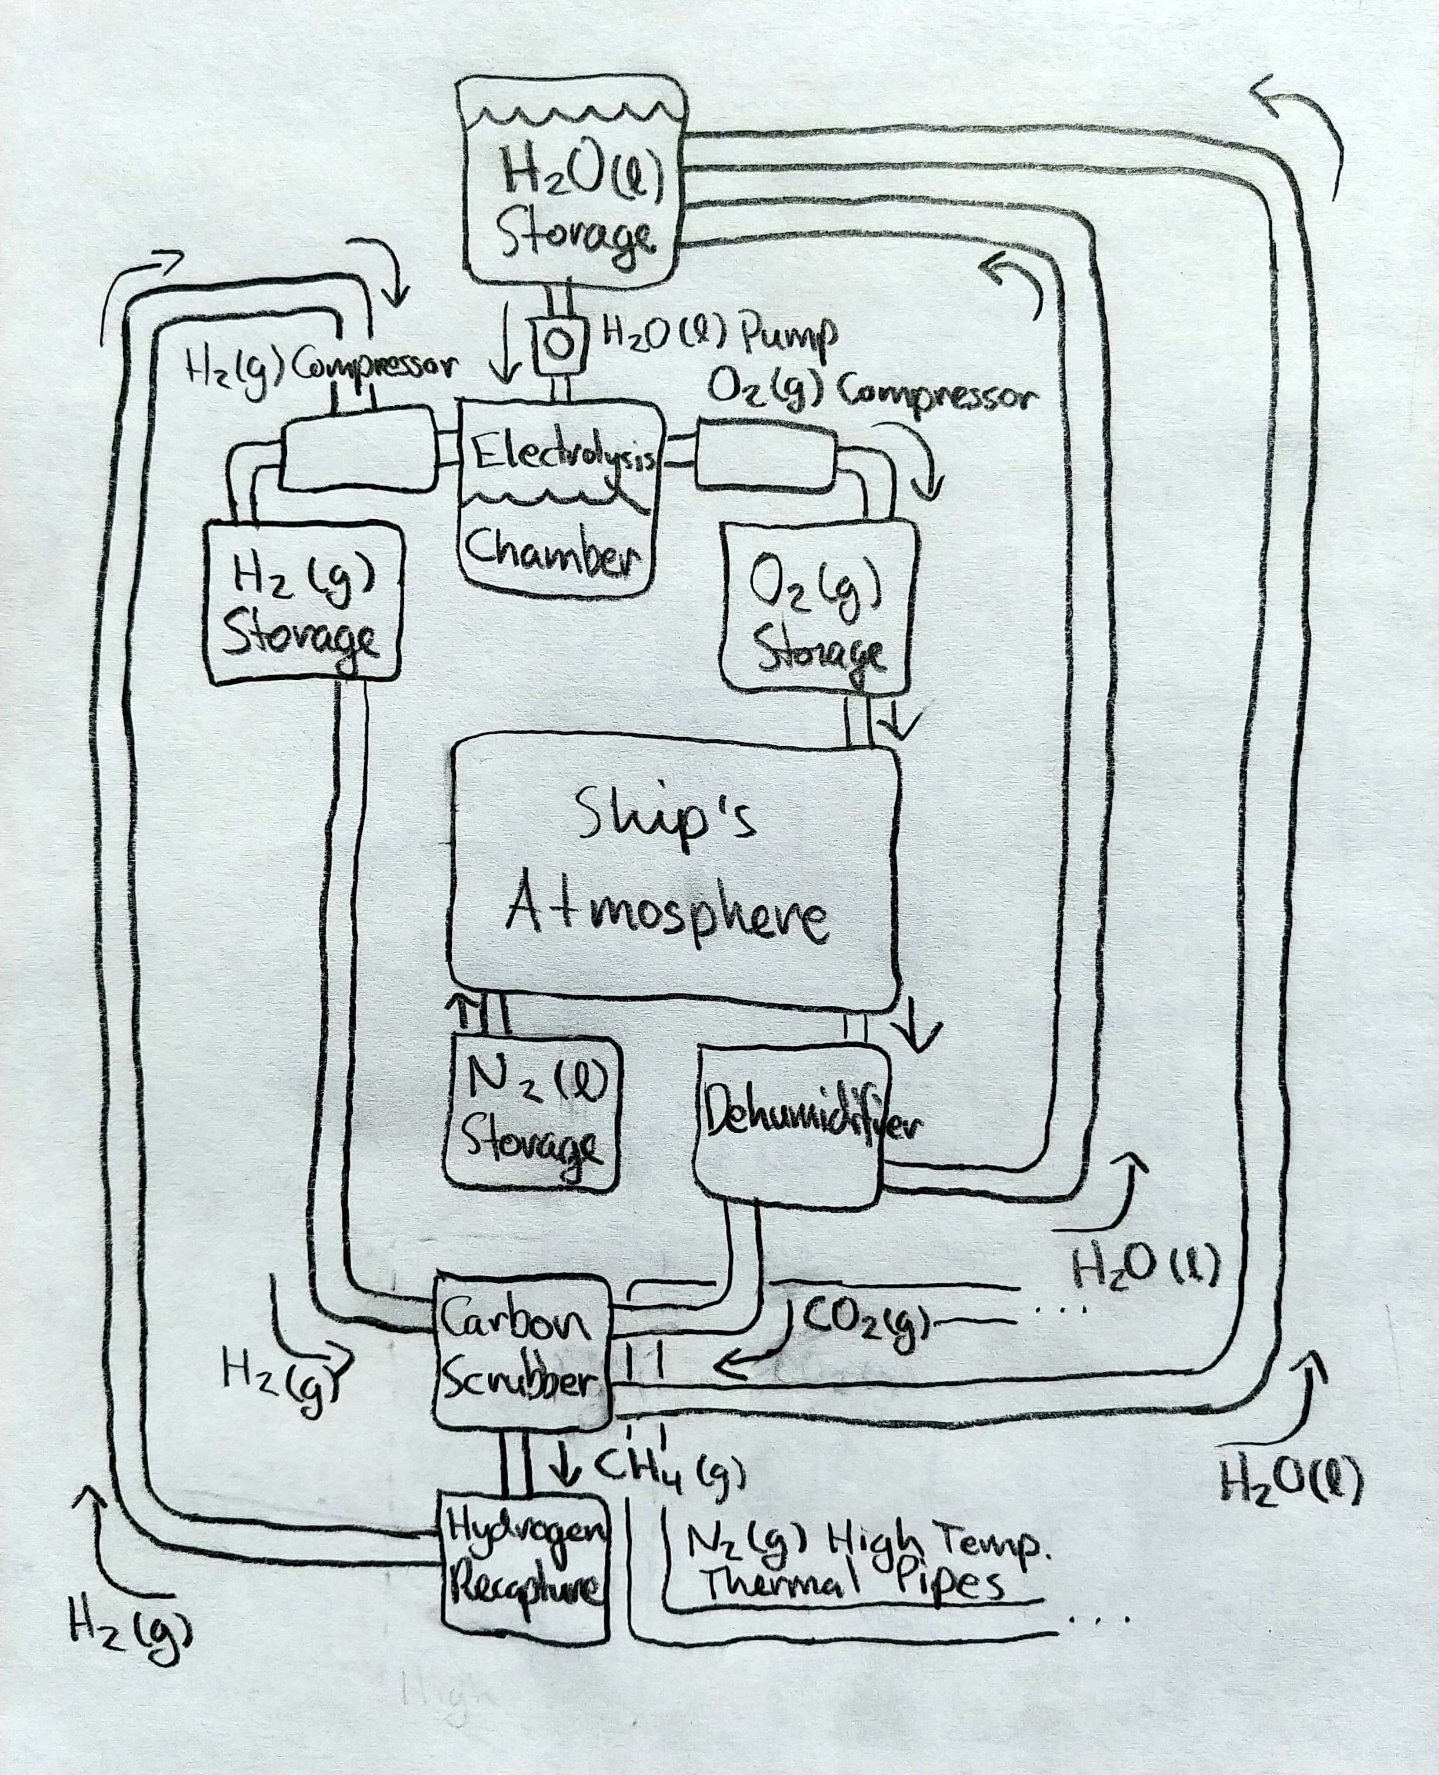
\includegraphics[scale=0.275]{Life_Support}

\vspace{0.5cm} \hspace{0.25\linewidth}
\begin{tabular}{@{} | c | l | c | @{}}
\toprule
\multicolumn{3}{|l|}{Table \ref{life} Life Support Components} \\
\toprule
1d30 & Component & Link \\
\midrule
1-2 & Electrolysis Chamber & \ref{life_electrolysis} \\
3-4 & Carbon Scrubber & \ref{life_c_scrubber} \\
5 & Hydrogen Recapture & \ref{life_h2_recapture} \\
6-7 & Dehumidifier & \ref{life_dehumidifier} \\
8-9 & Atmosphere & \ref{life_atmosphere} \\
\midrule
12-15 & H$_2$O (l) Storage & \ref{life_h2o_storage} \\
16 & H$_2$O (l) Pump & \ref{life_h2o_pump} \\
17-18 & H$_2$O (l) Pipe & \ref{life_h2o_pipe} \\
19-20 & H$_2$ (g) Storage & \ref{life_h2_storage} \\
21-22 & H$_2$ (g) Pipe & \ref{life_h2_pipe} \\
23 & H$_2$ (g) Compressor & \ref{life_h2_compressor} \\
24-25 & O$_2$ (g) Storage & \ref{life_o2_storage} \\
26-27 & O$_2$ (g) Pipe & \ref{life_o2_pipe} \\
28 & O$_2$ (g) Compressor & \ref{life_o2_compressor} \\
29-30 & N$_2$ (l) Storage & \ref{life_n2_storage} \\
\bottomrule
\end{tabular}

\vspace{0.3cm}
\begin{minipage}[t]{0.4\linewidth}
Fear
\begin{itemize}
\item The carbon scrubber \ref{life_c_scrubber} and the hydrogen recapture \ref{life_h2_recapture} components both handle extremely dangerous gases. The hydrogen and methane they use is handled at many hundreds of degrees centigrade, meaning the gases will instantly, violently explode if they come into contact with oxygen. Dealing with these systems requires the utmost care to avoid burn, explosion, or other extremely dangerous mishap.
\end{itemize}
\end{minipage} 
\begin{minipage}[t]{0.4\linewidth}
Anger
\begin{itemize}
\item The endless tiny pebbles contained in the dehumidifier \ref{life_dehumidifier} could be unimaginably annoying if they escape into the room. They will float around everywhere, bump into you while you work, and get into delicate machinery. A DM could poke a single player over and over with such a mishap, raising their frustration each time.
\end{itemize}
\end{minipage}

\begin{minipage}[t]{0.4\linewidth}
Isolation
\begin{itemize}
\item The quintessential way to make your players feel like they are alone in space, is to open up their room to the vacuum of space. Piercing or bludgeoning open the atmosphere \ref{life_atmosphere} of a room is a simple way to add tension while making sure the players are constantly reminded of just how close they are to cold, dead nothingness.
\end{itemize}
\end{minipage}
\begin{minipage}[t]{0.4\linewidth}
Duty
\begin{itemize}
\item The carbon scrubber \ref{life_c_scrubber} and the hydrogen recapture \ref{life_h2_recapture} components both contain layers of delicate catalysts. If a bludgeoning shot hits one of them, it can dent the sheets of metal out of shape, making them extremely difficult to remove. A character might be forced to open up the blazing-hot chamber and physically yank the sheets out in order to make sure the system keeps working.
\end{itemize}
\end{minipage}

\hspace{-18pt} \subsubsection{Electrolysis Chamber} \label{life_electrolysis} \vspace{-0.2cm}
A large vat of water serves as backup oxygen in case of failure. This is also needed because the one of the byproducts of the carbon stripping process is water. This water is split into its component gases which both go to temporary storage, to be then sent where needed.

\begin{equation}
2\ H_2O\ (l) \xrightarrow[]{electricity} 2\ H_2\ (g) + O_2\ (g) 
\end{equation}

An electrolysis chamber is composed of two filaments which gain opposite charges when electricity is applied. The electricity excites the water enough to split into gases, which are then collected. In case the electrolysis chamber needs to work very quickly, many layers of thin filaments are stacked on top of each other inside the chamber. 
\\ \pbhw
{A small hole is punctured through the casing. \newline \qtwo{A stream of water flows out.}{Either 1d2 H$_2$(g) or O$_2$(g) escapes.}}
{The casing is dented. \newline 1d4 = 1 A seal is broken. Either 1d3 H$_2$O(l), H$_2$(g), or O$_2$(g) escapes.}
{Heats very slowly. \newline 1d4 = 1 An electrical filament overheats. Either 1d2 H$_2$ or O$_2$ production is severely reduced.}
{Filaments must be regularly replaced. Container is subject to acids and oxidation.}


\vspace{-0.5cm} \hspace{-18pt} \subsubsection{Carbon Scrubber} \label{life_c_scrubber} \vspace{-0.2cm}
The carbon scrubbing process is composed of two parts. First carbon dioxide must be isolated from the air, and then the oxygen in it must be reclaimed. The first part of the process takes place in the \textit{Dehumidifier} \ref{life_dehumidifier}.

The second part of the scrubbing process isolates extracts oxygen from carbon dioxide by using the Sabatier reaction 
\begin{equation} \label{sabatier_reaction}
CO_2 + 4 H_2 \xrightarrow[\text{pressure}]{\text{400 C}} CH_4 + 2 H_2O
\end{equation}
A small pressurized chamber next to the radiator is kept very hot. Several thin plates of nickel act as catalysts for the reaction \cite{recycling_water_and_air}. Carbon dioxide is brought from the dehumidifier and allowed to pass over the catalysts in a hydrogen atmosphere. The reaction is allowed to go to near completion, and the methane then passes to the hydrogen recapture chamber.   
\\ \pbhw
{Extremely hot gas of either 1d2 H$_2$ or CH$_4$ escapes. As soon as the gas meets the oxygen of the air, it is so hot that it combusts, turning the jet of gas into a hydrogen or methane flamethrower.}
{The case is dented. \newline \hspace{3pt} 1d2 = 1. The denting is enough to make it difficult to remove layers of catalyst when they need to be replaced.}
{The heating of this component is kept tightly controlled. Any stray heat will transfer directly to the radiator to escape. }
{Plates require constant replacement due to cracking, wear, and depositing. }


\vspace{-0.5cm} \hspace{-18pt} \subsubsection{Hydrogen Recapture} \label{life_h2_recapture} \vspace{-0.2cm}
Once oxygen has been reclaimed from the carbon dioxide, hydrogen has taken the place of the oxygen. If the life support system intends to be fully self-sufficient, this hydrogen must be recaptured as well. If methane becomes hot enough in the absence of oxygen, it will decompose into solid carbon and hydrogen gas. 
\begin{equation} \label{anaerobic_decomposition_of_methane}
CH_4\ (g) \xrightarrow[anaerobic]{above\ 400\ C} C\ (s) + H_2\ (g)
\end{equation}

A second chamber sits next to the carbon scrubber chamber, which is also kept pressurized and much hotter, up to 900 \degree C. This chamber is similarly filled with plates of catalysts, though these plates are thinner and are made of iron or nickel in an alternating pattern. Methane enters, is heated, and the carbon is deposited on the surface of the catalyst sheets in the form of black soot, nanotubes, or graphite. The hydrogen can then return to storage while the carbon is scraped and shaken off. \cite{hydrogen_recapture}. 
\\ \pbhw
{A hole is pierced through the chamber, and a hot gas escapes of either 1d2 H$_2$ or CH$_4$. As soon as the hot gas meets the oxygen of the atmosphere, it combusts, turning the jet of gas into a flamethrower.}
{The chamber is dented. Carbon begins to accumulate at the point of denting, and is difficult to remove. \newline 1d2 = 1. The denting is enough to make it difficult to remove catalyst layers when they need replacement. }
{The heating of this component is also tightly controlled, so extra heat passes directly to the radiator.}
{Carbon is deposited directly onto the plates. The hot, pressurized plates are then shaken vigorously, and carbon is physically scraped off. This is a trifecta of erosion. Catalyst plates need to be replaced and recycled constantly.}


\vspace{-0.5cm} \hspace{-18pt} \subsubsection{Dehumidifier} \label{life_dehumidifier} \vspace{-0.2cm}
Humans mix water vapor and carbon dioxide into the air they breathe. The nitrogen and oxygen left in the gas can be reused, and will often mess with reclamation reactions, meaning the carbon dioxide and water must be physically separated from the rest of the atmosphere before they can be reused.

Eventually the air contained in all rooms in the ship must pass through a central dehumidifier chamber. This chamber is filled with a synthetic mineral called zeolite which soaks up water and carbon dioxide. Then the atmosphere can be vacated, and when the zeolite is reheated in the presence of a vacuum it will give off its stored water and carbon dioxide. The water is then condensed to a liquid and sent to storage, while the carbon dioxide is passed to the carbon scrubber.
\\ \pbhw
{The hole allows either air or carbon dioxide and water to escape.}
{The tiny mineral rocks are scattered everywhere throughout the room. They are smaller than pebbels and begin to bounce off everything in the room.}
{The rocks absorb heat well and will not melt for a long time.}
{Rocks become covered in stray grime and dust over time, becoming less absorbant. Rocks therefore must be replaced and recycled.}


\vspace{-0.5cm} \hspace{-18pt} \subsubsection{Atmosphere} \label{life_atmosphere} \vspace{-0.2cm}
Each individual room is hooked up to several things needed for life support. Every room needs to be pressurized and climate controlled. A room is connected directly to oxygen and nitrogen gas storage in case it needs to be repressurized, and it can be opened to the vacuum of space to depressurize as well. Each room has thermal cooling pipes for cooling the room and an electric heater in case a room needs to be quickly heated.

I recommend avoiding the more trivial items listed in the above paragraph. The following list describes how any room can be damaged by a weapon. Include this to add additional challenge to a problem. 
\\ \pbhw
{If a room's walls are pierced, it's only a matter of time before the room runs out of atmosphere.}
{If a bludgeoning shot has hit another system, it must have gone through the outer hull to get there. Make the hole small and the dent large so that every single bludgeoning shot doesn't immediately depressurize the room.}
{The room's heating system can only handle so much. If a system is heating up in a room, then the room is heating up too.}
{The structure of the outer hull degenerates over time like all things. Expect larger dents, and perhaps throw in a permanent crack or two. }


\vspace{-0.5cm} \hspace{-18pt} \subsubsection{H$_2$O (l) Storage} \label{life_h2o_storage} \vspace{-0.2cm}
This tank holds long-term reserve oxygen in case of emergency. It additionally collects the byproducts of the carbon scrubbing process and the water vapor that humans breathe out into the atmosphere.
\\ \pbhw
{The outside container is punctured. Maintaining pressure becomes difficult, so only passive flow occurs. \newline 1d2 = 1 The inner lining is punctured too. Liquid escapes into the container vat, and passive flow is reduced.}
{The outer container is dented, reducing maximum capacity. If the tank is full, this sends a pressure wave to break the weakest point of the tank, its outflow valve. 1d4 = 1 The outflow valve breaks and water surges out.}
{Water absorbs huge amounts of heat before its temperature rises dangerously. Little effect.}
{Water erodes any container it's in relatively quickly. This is particularly apparent around the input and output valves.}


\vspace{-0.5cm} \hspace{-18pt} \subsubsection{H$_2$O (l) Pump} \label{life_h2o_pump} \vspace{-0.2cm}
It's a big wet fan.
\\ \pbhw
{One of the turbine blades has a hole pierced through it. \newline 1d4 = 1 The hole is enough to shatter the blade when it starts spinning too quickly. }
{The turbine comes screeching to a halt. A total of 1d4 out of 8 blades are damaged.}
{The turbine will transfer heat to the water. }
{The turbine erodes quickly from the water.}


\vspace{-0.5cm} \hspace{-18pt} \subsubsection{H$_2$O (l) Pipe} \label{life_h2o_pipe} \vspace{-0.2cm}
It's a pipe that carries water.
\\ \pbhw
{Water spills out.}
{Limits water flow slightly.}
{Transfers heat to the railgun when sprayed on it.}
{Water wears pipes decently quickly.}


\vspace{-0.5cm} \hspace{-18pt} \subsubsection{H$_2$ (g) Storage} \label{life_h2_storage} \vspace{-0.2cm}
Hydrogen is slightly less terrifying to store as a gas than as a liquid, but should still be handled with utmost care. 
\\ \pbhw
{Hydrogen gas escapes.}
{The tank is dented. \newline 1d4 = 1. The pressure increase is enough to break the output valve, letting hydrogen gas gush into the air.}
{Hydrogen gas heats very quickly and will push out immense pressures. \newline 1d4 = 1. The pressure increase is enough to break the output valve, letting hydrogen gas gush into the air.}
{Hydrogen wears containers very little.}


\vspace{-0.5cm} \hspace{-18pt} \subsubsection{H$_2$ (g) Pipe} \label{life_h2_pipe} \vspace{-0.2cm}
Hydrogen gas flows through this pipe.
\\ \pbhw
{Hydrogen gas escapes.}
{The flow is restricted. \newline 1d2 = 1. The blow is enough to break a seal, letting hydrogen gas escape into the atmosphere.}
{The hydrogen will heat up a lot and transfer that increased temperature and pressure to the system downstream.}
{Little wear.}


\vspace{-0.5cm} \hspace{-18pt} \subsubsection{H$_2$ (g) Compressor} \label{life_h2_compressor} \vspace{-0.2cm}
For hydrogen gas to be stored in a tank, something must compress it to a higher pressure than the tank before it will flow into the tank. A typical compressor is a fan that blows strongly, but such blades could disturb the hydrogen into combustion. Instead, a slow-moving piston is used to compress the gas.
\\ \pbhw
{\qtwo{The hole is behind the piston, preventing it from retracting behind that point.}{The hole is in front of the piston. Super-compressed hydrogen gas escapes extremely quickly. The sheer speed of the hydrogen escaping would likely be enough to ignite it on fire.}}
{\qtwo{The dent prevents the piston from retracting fully.}{The dent prevents the piston from compressing fully.}}
{The pressure of the hydrogen will increase. Luckily, that is what this system is designed to handle.}
{Pistons require lubrication and the seal requires maintenance.}


\vspace{-0.5cm} \hspace{-18pt} \subsubsection{O$_2$ (g) Storage} \label{life_o2_storage} \vspace{-0.2cm}
Oxygen gas is stored in a container before it is piped into the atmosphere.
\\ \pbhw
{Oxygen gas escapes.}
{The tank is dented. \newline 1d4 = 1. The denting sends a pressure wave strong enough to break the output valve, letting oxygen gas escape.}
{The oxygen will absorb the heat slowly, and then will transfer it to the atmosphere of the rooms.}
{Oxygen is corrosive but the tank is designed to mitigate that.}


\vspace{-0.5cm} \hspace{-18pt} \subsubsection{O$_2$ (g) Pipe} \label{life_o2_pipe} \vspace{-0.2cm}
This pipe carries oxygen gas.
\\ \pbhw
{Oxygen gas escapes.}
{Restricts flow. \newline 1d2 = 1. The blow is enough to break a seal, and oxygen gas escapes.}
{The oxygen gas transfers the heat to the atmosphere of the room it is entering.}
{Oxygen is corrosive but the pipe is designed to mitigate that.}


\vspace{-0.5cm} \hspace{-18pt} \subsubsection{O$_2$ (g) Compressor} \label{life_o2_compressor} \vspace{-0.2cm}
A similar oxygen compressor works in parallel with the hydrogen compressor, pushing oxygen gas into storage.
\\ \pbhw
{\qtwo{The hole is behind the piston, stopping it from retracting behind that point.}{The hole is in front of the piston, allowing super-compressed oxygen gas to escape very quickly.}}
{\qtwo{The dent prevents the piston from retracting fully.}{The dent prevents the piston from compressing fully.}}
{The oxygen heats up, increasing the pressure, but this device is designed to handle high pressures.}
{Oxygen corrodes things that aren't designed to hold it.}


\vspace{-0.5cm} \hspace{-18pt} \subsubsection{N$_2$ (l) Storage} \label{life_n2_storage} \vspace{-0.2cm}
A vat of liquid nitrogen supplies extra air for the ship. The vat is kept very close to boiling temperature, and the gas that evaporates naturally flows into each room. This nitrogen should only be used if a room needs to be repressurized after its air has been evacuated.
\\ \pbhw
{Liquid nitrogen spills out. It immediately freezes anything it touches. Great billows of thick white gas engulf the room, significantly lowering the temperature and completely blocking vision.}
{The tank is dented. \newline 1d4 = 1. The dent sends a pressure wave enough to burst a seal, and liquid nitrogen spills out. See \textit{piercing} effects above.}
{The nitrogen immediately begins to boil. The cooling coils can deal with heat gain due to passive influences, but if something actively adds heat to this tank, they could not keep up. The boiling nitrogen will raise the pressure of its container significantly. \newline 1d2 = 1. The rise in pressure is enough to burst a seal, letting liquid nitrogen spill out. See \textit{piercing} effects above.}
{Such cold liquids wear little, but their containers become brittle over time.}


\newpage
\subsection{Electrical Grid} \label{grid}

Every single system aboard the ship requires some form of electricity to function properly. A small, self-contained nuclear reactor gives the ship more power than it knows what to do with. This supplies power in the form of a central high-voltage AC line. Weaponry taps directly into this line, though converting it to DC power first. A transformer lowers the voltage for the less intense systems and computers.

\vspace{0.2cm}
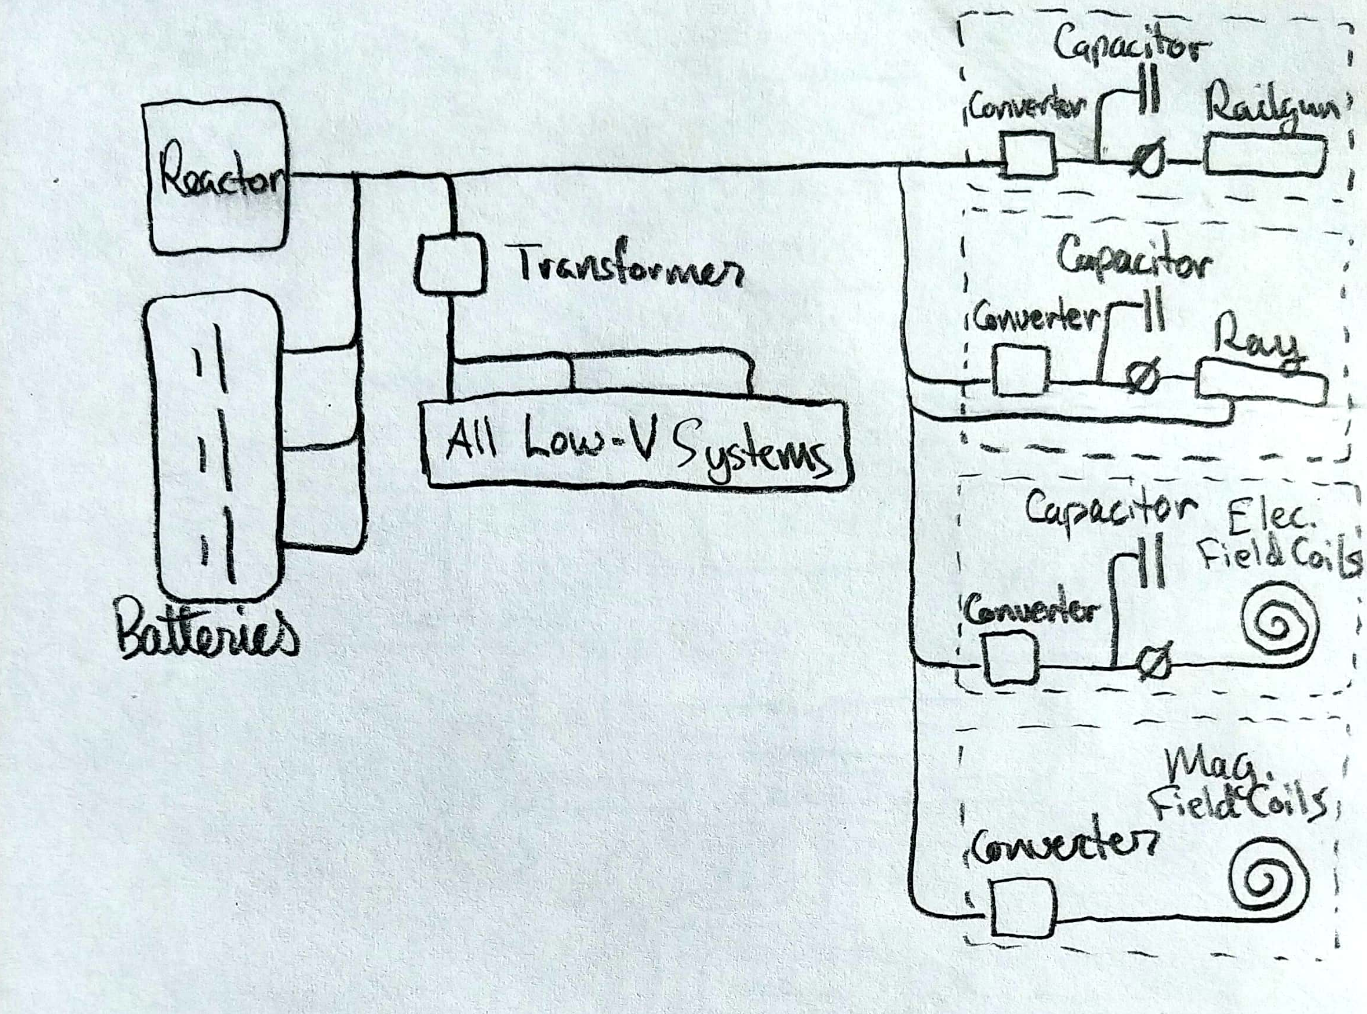
\includegraphics[scale=0.3]{Electrical_Grid}

\vspace{0.5cm} \hspace{0.25\linewidth}
\begin{tabular}{@{} | c | l | c | @{}}
\toprule
\multicolumn{3}{|l|}{Table \ref{grid} Electrical Grid Components} \\
\toprule
1d20 & Component & Link \\
\midrule
- & Reactor & \ref{grid_reactor} \\
1-4 & Batteries & \ref{grid_batteries} \\
5-6 & Transformer & \ref{grid_transformer} \\
7-8 & Converter & \ref{grid_converter} \\
9-10 & Capacitor & \ref{grid_capacitor} \\
11-12 & Electric Field Generator & \ref{grid_e_field_generator} \\
13-16 & Magnetic Field Coils & \ref{grid_m_field_coils} \\
17-19 & Wiring & \ref{grid_wiring} \\
20 & Heavy Wiring & \ref{grid_heavy_wiring} \\
\bottomrule
\end{tabular}

\vspace{0.3cm}
\begin{minipage}[t]{0.4\linewidth}
Fear
\begin{itemize}
\item While it would match with the theme of fear, I recommend avoiding damaging the reactor \ref{grid_reactor}, as it would immediately turn the RPG into a post-apocalyptic horror scenario. Instead, the extremely cold, humming magnetic field coils \ref{grid_m_field_coils} provide sufficient tension while keeping the danger (relatively) low. A single puncture or a stray source of heat can turn this system into a frozen helium bomb. 
\end{itemize}
\end{minipage} 
\begin{minipage}[t]{0.4\linewidth}
Anger
\begin{itemize}
\item Any time a component with wiring is damaged by either piercing or bludgeoning, there is a likely chance that electrical sparks fly. If things keep going wrong in this system for a character, consider continually shocking them, with the shocks getting worse the more angry and sloppy the character gets.
\end{itemize}
\end{minipage}

\begin{minipage}[t]{0.4\linewidth}
Isolation
\begin{itemize}
\item A single line connects the reactor to the rest of the ship. If this line is broken or stopped, every single system on the ship loses power and many of them stop immediately. While batteries can be used as a backup to maintain power for a while, they can't sustain weaponry during combat. If the power goes out, the ship is completely stranded with no communication or control.
\end{itemize}
\end{minipage}
\begin{minipage}[t]{0.4\linewidth}
Duty
\begin{itemize}
\item Many different coils exist throughout the electrical grid, including in the transformer \ref{grid_transformer}, electric field generator \ref{grid_e_field_generator}, and magnetic field coils \ref{grid_m_field_coils}. If these are bent out of shape, it is likely they come into contact with another metal object. This short circuits the coil and causes a part of it to become very hot very quickly. A brave soul might have to bend a coil back into shape by hand while it's searing hot.
\end{itemize}
\end{minipage}

\hspace{-18pt} \subsubsection{Reactor} \label{grid_reactor} \vspace{-0.2cm}
The part of the ship that generates electricity is a self-contained nuclear reactor. A ship's engineer need only plug it in to the electrical and thermal grids, and it works. The reactor typically produces an excess of electrical energy for the ship, so that nobody should worry about running out. A nuclear reactor is a complicated thing in itself, and any damage to it could be catastrophic to the crew inside. As a result, avoid having the reactor undergo any problems. It is by far the safest hardware on the ship, with the worst consequences if broken.

\vspace{-0.5cm} \hspace{-18pt} \subsubsection{Batteries} \label{grid_batteries} \vspace{-0.2cm}
If the reactor needs to temporarily shut down, the ship can run off of a store of batteries for a few hours. Using these batteries to shoot weaponry will make them deplete significantly faster.
\\ \pbhw
{Battery acid spills out from a total of 1d4 batteries.}
{One battery is smashed to pieces. A total of 1d4 batteries are ripped from their sockets and scattered, and 1d8 more are dislodged from place but are still connected.}
{Batteries do not fare well under heat. Expect eventual leakage and expansion.}
{Batteries lose capacity over time, and must be replaced.}


\vspace{-0.5cm} \hspace{-18pt} \subsubsection{Transformer} \label{grid_transformer} \vspace{-0.2cm}
Power from the reactor comes at high voltage for the more demanding parts of the ship. The majority of systems require only a computer or minor electrical parts, and so only need low-voltage wiring. A transformer turns the high voltage reactor output into low voltage electricity for most of the ship to use.

A transformer is composed of a large hunk of metal with two coils wrapped entirely around it on separate sides. 
\\ \pbhw
{\qeq{1d4}{1-2.}{The chunk of metal in the middle is pierced, with little effect.}{3.}{The high voltage coil is pierced, significantly reducing current flow.}{4.}{The low voltage coil is pierced, significantly reducing current output.}{}{}}
{Will likely dent something enough that a coil begins to touch the metal hunk. This will short circuit the system and may melt or burn a section of the coil.}
{The metal chunk will absorb much heat.}
{Little wear.}


\vspace{-0.5cm} \hspace{-18pt} \subsubsection{Converter} \label{grid_converter} \vspace{-0.2cm}
The main electrical grid of the ship uses AC power, which needs to be converted to DC power for a few systems, including the 1d4 railgun, ray, electric field generator, and magnetic field coils. A converter consists of a diode bridge, containing four diodes, and a capacitor. 
\\ \pbhw
{\qeq{1d5}{1-4.}{A diode is hit. These are impractical to fix and simply need replacing. The wires are unfortunately quite thick in order to handle such currents and voltages, and so need thick wire cutters and proper soldering to replace.}{5.}{The capacitor is hit. This is a heavy-duty capacitor and there are plenty of replacement capacitors, though again soldering is required for a proper fix on such a critical part.}{}{}{}{}}
{Mostly only the casing is dented. \newline 1d4 = 1 A single wire is disconnected somewhere.}
{The wires are thick and used to being heated significantly from the huge current.}
{Wiring and especially soldering joints require maintenance and occasional replacement.}


\vspace{-0.5cm} \hspace{-18pt} \subsubsection{Capacitor} \label{grid_capacitor} \vspace{-0.2cm}
Certain systems need a huge surge of current and voltage in a fraction of a second, which is perfect for a capacitor. A large array of capacitors are connected in parallel and charged by the DC power coming from the converter before it. A capacitor is included in the 1d3 railgun, ray, and electric field generator (sub)systems.
\\ \pbhw
{A single capacitor is hit and requires replacement.}
{A total of 1d4 different capacitors are all damaged by the hit, and many are scattered and displaced. A few wires become tangled, and some are pulled out.}
{The thin metal plates of a capacitor will melt under focused heat, though capacitors are kept far from the hot rails.}
{Capacitors burn out and wires corrode.}


\vspace{-0.5cm} \hspace{-18pt} \subsubsection{Electric Field Generator} \label{grid_e_field_generator} \vspace{-0.2cm}
This particular design of electric field generator uses a strong electromagnet. Energy is dumped rapidly into the magnet coil, and the rapid rise in a magnetic field can generate a strong electric field as well. An electric field generator coil is included at two opposite parts of the ship where the magnetic fields of the ship end up accumulating hot particles. Strong bursts of electric field push the particles away when the accumulations become too large.
\\ \pbhw
{The wiring of the electromagnet is pierced. The casing is open, meaning sparks can fly. \newline 1d2 = 1. The piercing completely nicks the wiring, stopping all electrical flow.}
{The electromagnet is bent out of shape, altering the direction that it accelerates away the hot ions near it. \newline 1d2 = 1. The coil is bent completely out of shape, and will not sufficiently push away the hot ions.}
{The wiring will warp and can eventually short circuit.}
{Such swings in current will wear even a strong wire decently quickly. }


\vspace{-0.5cm} \hspace{-18pt} \subsubsection{Magnetic Field Coils} \label{grid_m_field_coils} \vspace{-0.2cm}
The ship is wrapped in long coils that envelop the ship in magnetic fields. When hot ions arrive from the sun or from enemy ray shots, they are deflected by the magnetic fields. 

Ray shots arrive far too quickly to be able to predict. As a result, the magnetic fields must be kept up at all times. This is possible by keeping the magnetic field coils cooled so much that the helium inside becomes a superconductor. A ship can dump excess electrical energy into the superconductor, and very little of that energy will be dissipated over time. Instead that energy will all go toward deflecting any ions that arrive, whenever they arrive.
\\ \pbhw
{Liquid helium escapes. Whether it escapes into the vacuum of space or into a pressurized atmosphere, it instantly evaporates into a gas. }
{The coils become dented, limiting helium flow rate and thus magnetic field strength. Warms up the coil noticeably as well, temporarily stopping its use.}
{Keeping the coils so incredibly cool for so long is difficult, and the more energy the ship dumps into the coils the warmer they become. As a result, this defense mechanism works in the beginning of the fight, but rapidly falls behind as the helium loses its superconducting state and must be slowly cooled again. Once it stops superconducting, all the magnetic fields die.}
{Casing becomes brittle from the cold. Helium escapes slightly, but over time this is noticeable.}


\vspace{-0.5cm} \hspace{-18pt} \subsubsection{Wiring} \label{grid_wiring} \vspace{-0.2cm}
The most common wiring carries low voltage electricity to the majority of systems on the ship.
\\ \pbhw
{The wire is nicked, reducing current flow significantly.}
{The wire is yanked out of place and its 1d2 out of its two connections on either side are ripped out.}
{The wire's covering will burn before the wire melts.}
{Little wear, mostly on the connections between wires and other things.}


\vspace{-0.5cm} \hspace{-18pt} \subsubsection{Heavy Wiring} \label{grid_heavy_wiring} \vspace{-0.2cm}
Heavy wiring carries high voltage electricity from the reactor to the systems of the ship that demand more power.
\\ \pbhw
{A small section of the wiring is pierced, doing little. Sparks can now easily jump out of the hole due to the enormous voltage.}
{The wiring takes the brunt of the hit. This can split open its rubber casing, allow sparks out. Additionally it can smash wires inside or break them, reducing flow. Finally it can sever the connection on either end of the wiring.}
{The metal in the wire will absorb much heat, though the rubber will still burn first.}
{Requires regular replacement.}


\newpage
\subsection{Fighter AR Display} \label{fighter}

A fighter pilot in open space would look around him outside a glass window and see the pitch black void of space. If there were any ships visible, they would be so far away as to be minuscule specks, and often are only partially lit by the sun. As a result, a collection of videogame designers and military simulation designers worked together to create an alternate-reality virtual battlefield for pilots to view in real-time.

Now, when a pilot looks out their visor, they see any ships nearby as highlighted outlines, with indications of their direction of movement and orientation, and they instead of an empty void they see a field of spaced lines as a coordinate system around them. The picture below is a third-person view of a battlefield with most components of the AR display drawn and labeled.

\vspace{0.2cm}
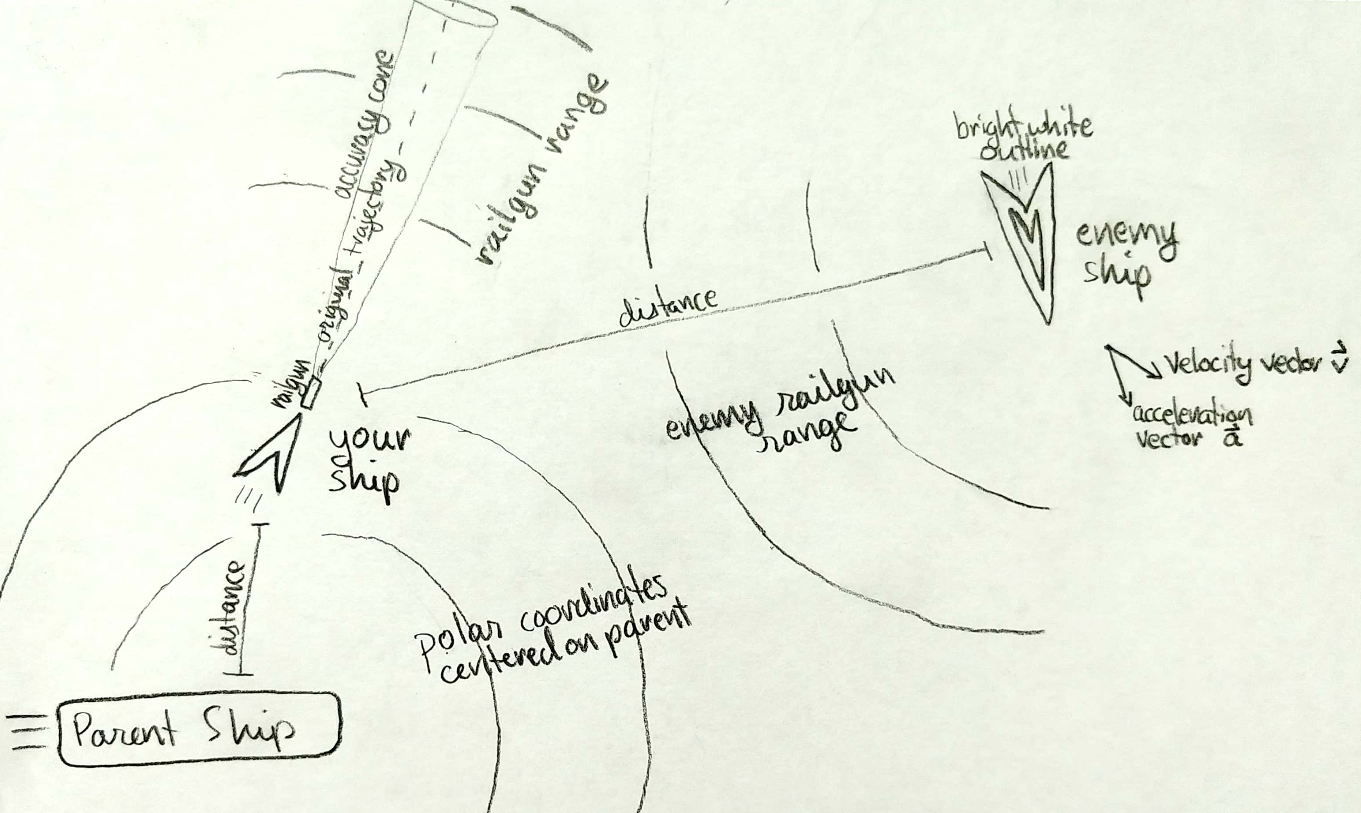
\includegraphics[scale=0.3]{Fighter_AR_Display}

\vspace{0.5cm} \hspace{0.25\linewidth}
\begin{tabular}{@{} | c | l | c | @{}}
\toprule
\multicolumn{3}{|l|}{Table \ref{fighter} Fighter AR Components} \\
\toprule
1d10 & Component & Link \\
\midrule
1 & Positioning & \ref{fighter_positioning} \\
2 & Vectoring & \ref{fighter_vectoring} \\
3 & Ranging & \ref{fighter_ranging} \\
4-5 & Aiming & \ref{fighter_aiming} \\
6 & Warning & \ref{fighter_warning} \\
7 & Evading & \ref{fighter_evading} \\
8-9 & Controlling & \ref{fighter_controlling} \\
\bottomrule
\end{tabular}

\vspace{0.3cm}
\begin{minipage}[t]{0.4\linewidth}
Fear
\begin{itemize}
\item Many parts of the ship act without the will of the pilot. The ship might suddenly jump to dodge \ref{fighter_evading} out of the way of a shot, and might start aiming the railgun \ref{fighter_aiming} when it detects an enemy in front of it. The ship as a whole, a unit of engineering marvel, might start to seem like a living, moody thing. Focus on its indifference to the pilot, choosing different things and jarring the pilot during thought. Such a disconnect between rider and horse is scary on its own - a disconnect like this between pilot and ship is haunting.
\end{itemize}
\end{minipage} 
\begin{minipage}[t]{0.4\linewidth}
Anger
\begin{itemize}
\item If the reader has debugged \ref{fighter_computer_bug_types} any program, they will know that it can be incredibly frustrating. Consider having the same type of bug appear several times in a row, possibly for the same reason, to irritate them. Another option is to have one specific system be made by an incompetent programmer, and this becomes more and more apparent as the pilot finds bug after bug in that one system.
\end{itemize}
\end{minipage}

\begin{minipage}[t]{0.4\linewidth}
Isolation
\begin{itemize}
\item If a sufficient terrible problem leaves the pilot out of control \ref{fighter_controlling} of the ship, it will drift away into the void. The pilot will have to be recovered by another ship long after the combat is finished.
\end{itemize}
\end{minipage}
\begin{minipage}[t]{0.4\linewidth}
Duty
\begin{itemize}
\item In the case that the aiming system \ref{fighter_aiming} of the ship keeps failing, a brave fighter pilot might have to raise up their visor and fire a key shot at the enemy ship, without any computer assistance whatsoever. 
\end{itemize}
\end{minipage}

\subsubsection{Combat System} \label{fighter_combat_system}

The following is a brief description of a combat system for fighter ships. I recommend focusing on the bugfixing, problem solving, and outer-space acrobatics problems instead of the combat.

Each turn of fighter combat, choose \textit{up to two} of the following actions to take.
\begin{itemize}
\item \textit{Thrust}. Choose a location and fire your engines towards it, or halt to a stop, or turn your velocity vector. Firing your engines requires focusing on what direction to fire and how to manage your ships position and velocity.
\item \textit{Fire}. Choose an enemy and fire the fighter's railgun at them. If the enemy is close enough, the player can choose which system of the ship to hit. If the enemy is medium range, the player can attempt to predict which direction the enemy will dodge, and if they predict it correctly they hit. When choosing a direction, something simple like choosing one of up, down, left, or right is sufficient, and results in a 1/4 chance of hit. Optionally 8-fold direction can be used, in which case I recommend the chance of hit to be 3/8, so that choosing adjacent directions results in a hit (If enemy dodges N, then firing at any of NW, N, or NE will hit it).
\item \textit{React - Dodge}. Take no immediate action. Instead wait for the next shot to be fired at you, and attempt to dodge it. If the enemy is close enough when the shot is fired, dodging is useless. If the enemy is medium range, the player chooses a direction to dodge. If the enemy predicts the correct direction, they will hit you, and otherwise will miss. Again, either the 4-fold direction 1/4 chance or 8-fold 3/8 chance method can be used.
\item \textit{React - Deflect}. Take no immediate action. Instead aim the fighter's railgun precisely at an enemy railgun. When that railgun fires, the thermal imaging cameras on the railgun will trigger it to immediately fire, and the two shots will collide in mid-space, deflecting them both in random directions. This method allows a ship to theoretically avoid two different shots each turn, if it does nothing else on its turn.
\end{itemize}

\vspace{0.2cm} \hspace{-17pt} Note that using either the engine or the railgun excessively in one turn will put stress on it. Take the following actions if these two specific actions are taken.
\begin{itemize}
\item \textit{Fire and React - Deflect}. If the pilot both fires a shot and then ends up firing a second deflection shot before their next turn, then the railgun will undergo heat stress. To be brutal, see the \textit{T} section of \ref{railgun_rails}.
\item \textit{Thrust and React - Dodge}. If the pilot both fires the engines to thrust and then ends up having to dodge a shot before their next turn, then the engine will undergo heat stress. To be brutal, see the \textit{T} section of \ref{engine_exhaust}.
\end{itemize}


\subsubsection{Computer Damage Types} \label{fighter_computer_damage_types}

The damage types used for other systems are not particularly applicable to computer systems. Here \textit{Wear} damage will be split into two parts: stray UV radiation from the sun and stray magnetic fields from other ships. These five will form the base damage types.

Each base damage type can cause a number of different secondary problems, which ultimately then cause a result problem. There are very few result problems, meaning knowing the full path of the problem is important. The following table summarizes the base damage types, secondary problems, and result problems, as well as which leads to which.


\vspace{0.2cm} \hspace{0.1\linewidth}
\begin{tabular}{| l |}
\toprule
Table \ref{fighter_computer_damage_types} Computer Damage Types \\
\midrule
\hspace{10pt} base problem \hspace{40pt} secondary problem \hspace{10pt} result problem \\
\midrule
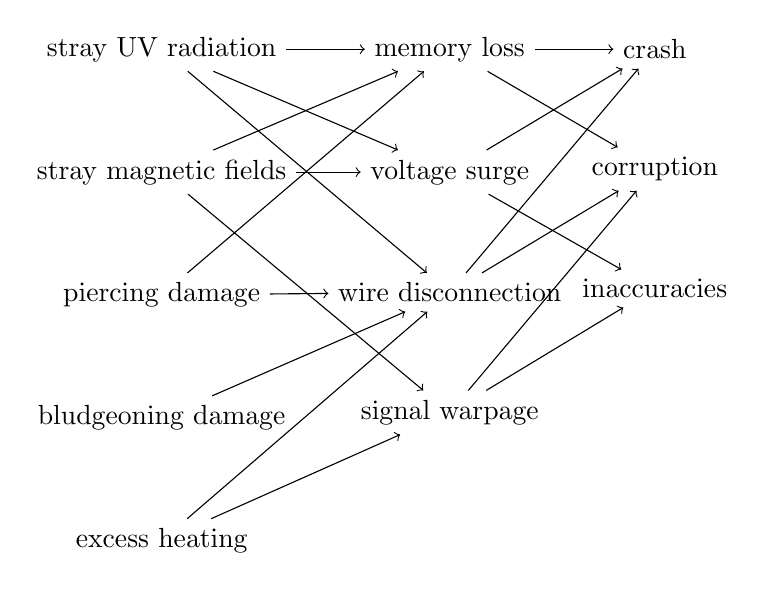
\begin{tikzpicture}
\node(A){stray UV radiation};
\node(B)[below=of A]{stray magnetic fields};
\node(C)[below=of B]{piercing damage};
\node(D)[below=of C]{bludgeoning damage};
\node(E)[below=of D]{excess heating};

\node(F)[right=of A]{memory loss};
\node(G)[right=of A, below=of F]{voltage surge};
\node(H)[right=of A, below=of G]{wire disconnection};
\node(I)[right=of A, below=of H]{signal warpage};

\node(J)[right=of F]{crash};
\node(K)[right=of F, below=of J]{corruption};
\node(L)[right=of F, below=of K]{inaccuracies};

\draw [->] (A) -> (F);
\draw [->] (A) -> (G);
\draw [->] (A) -> (H);
\draw [->] (B) -> (F);
\draw [->] (B) -> (G);
\draw [->] (B) -> (I);
\draw [->] (C) -> (F);
\draw [->] (C) -> (H);
\draw [->] (D) -> (H);
\draw [->] (E) -> (H);
\draw [->] (E) -> (I);

\draw [->] (F) -> (J);
\draw [->] (F) -> (K);
\draw [->] (G) -> (J);
\draw [->] (G) -> (L);
\draw [->] (H) -> (J);
\draw [->] (H) -> (K);
\draw [->] (I) -> (K);
\draw [->] (I) -> (L);
\end{tikzpicture} \\
\bottomrule
\end{tabular}

\vspace{0.2cm}
Base problems
\begin{enumerate}[leftmargin=4cm]
\item [stray UV radiation] - What would normally be blocked by the atmosphere is instead allowed to ravage the precise electronics of a ship. This is the same radiation that gives you a sunburn, which can cause bits to be changed, wires to undergo a surge, and even fry a wire.
\item [stray magnetic fields] - In strong areas of a planet's magnetic field or when very close to another ship, the electrons moving in precise patterns in the electronics suddenly experience a magnetic force, throwing them in random directions as the ship moves through it.
\item [piercing damage] - Physical piercing damage can damage hard drives and disconnect wires.
\item [bludgeoning damage] - Dents can disconnect wires and can totally destroy some parts, but otherwise they do little.
\item [excess heating] - A processor that gets too hot will see its wires rapidly melt if it's not completely shut down. Additionally the temperature can interfere with receiving and sending signals with antannas. 
\end{enumerate}

\vspace{0.2cm}
Secondary problems
\begin{enumerate}[leftmargin=4cm]
\item [memory loss] - Permanent or temporary memory of the computer can be deleted by base damages. This results in the computer not being able to find something, finding nothing when it does, or straight up crashing.
\item [voltage surge] - A surge of voltage in the wrong direction can be disastrous. If writing data or performing a particularly important calculation, one of these surges could cause a completely wrong number to be calculated. This is as long as the surge is weak enough to not fry the wire completely, resulting in a wire disconnection.
\item [wire disconnection] - A wire is completely disconnected as a result of melting, frying, or being physically yanked out. This typically instantly crashes the system, and if not it will result in warped results and certain impossible operations.
\item [signal warpage] - The communications signals that should be coming to the player are being warped by faulty parts or magnetic field interference. As a result voice communications are distorted, your measured distance to the parent ship and thus also your own velocity (calculated based on this distance) will be off, and any further orders or transferred data may be inaccurate.
\end{enumerate}


\vspace{0.2cm}
Result problems
\begin{enumerate}[leftmargin=4cm]
\item [crash] - One particular program of the whole completely crashes, stopping it until it can be rebooted. If not bugfixed, the problem will arise again guaranteed.
\item [corruption] - The computer has failed to find something or found nothing where it should have been. This results in basic textures being displayed, missing data points, and warped lines displayed on screen. If not bugfixed, a restart may (1d2 = 2) successfully reformat everything and fix the problem, or it may be unsucessful.
\item [inaccuracies] - While all the components are properly working, wrong numbers keep consistently getting spit out. This results in warped voices, missed shots, and an inaccurate depiction of the battlefield.
\end{enumerate}


\subsubsection{Computer Bug Types} \label{fighter_computer_bug_types}

A DM can cause physical damage to the computer systems of the fighter, as described in the above section, but they can also let software issues get in the way as well. The following is a list of problems of varying severity in no particular order which can serve as problems. These problems have wildly differing amounts of work needed to fix them: a versioning issue can be fixed in ten seconds by downloading the right version, while a timekeeping issue can be a needle in a haystack to solve.

\begin{minipage}[t]{0.45\linewidth}
\begin{itemize}[leftmargin=0cm]
\item memory leak - An issue in the program causes more and more memory to be needed, eventually slowing down the entire system to a crawl.
\item buffer overflow - The program begins writing memory beyond the designated area that it is currently working on. Causes corruption of data, changing file headings to make them disappear before obliterating their contents.
\item floating point rounding - A comparison in the code expects exact equality between two numbers on either side of the equals sign in an equation. This should be theoretically true, but practically floating point numbers can't store certain numbers exactly, so equality does not hold. 
\item numerical instability - An algorithm is theoretically sound, except that at some stage it rounds a number, causing the accuracy of the algorithm to drift significantly over time.
\item off-by-one - A long list of numbers should have exactly one more or one less element than it does, leaving the program in a question of what to do. 
\end{itemize}
\end{minipage}
\begin{minipage}[t]{0.5\linewidth}
\begin{itemize}[leftmargin=0.5cm]
\item null pointer - A program searched for an object in memory but found nothing in its place. This is typically the error thrown when memory is damaged, and usually results in a crash right away.
\item divide-by-zero - A programmer lazily never considered that a certain equation could result in dividing by zero. The computer recognizes this is an error and won't completely crash, but won't continue either.
\item timekeeping - Even the slightest error in a clock will add up very noticeably over time. Since the clock is used for everything relating to the equations of motion, trajectories will become wrong. This is especially important for spacefaring vessels, which have to adjust their time dynamically as a result of their height in orbit and their speed. 
\item syntax - The programmer literally used the wrong words. This can be as obvious as a straight up typo, to something more subtle like i = 1 vs i == 1.
\end{itemize}
\end{minipage}

\begin{minipage}[t]{0.45\linewidth}
\begin{itemize}[leftmargin=0cm]
\item integer overflow - An integer can become so large, so unbelievably large that the programmer never anticipated that it could be possible, that it will flip over and either return to 0 or become an enormous negative number. This sudden swing can lead to laughably huge inaccuracies. 
\item improper units - One part of the computer expects a certain unit, while another part hands it a different unit. While this problem may seem trivial, over the course of history it has caused multiple multi-million dollar space exploration missions to catastrophically fail.
\item type formatting - A malicious user or stray corruption of data causes a random character to be inserted into a text being displayed. If the wrong character, and especially if the programmer never anticipated it, this can cause surprisingly frequent crashes.
\item versioning - A piece of software is using the wrong version of another API or library. This can lead to security issues and inaccuracies if major bugs have been recently fixed. 
\end{itemize}
\end{minipage}
\begin{minipage}[t]{0.5\linewidth}
\begin{itemize}[leftmargin=0.5cm]
\item infinite loop - Somewhere in the program an unforeseen loop occurs which cannot be exited. Modern operating systems will stop this after a number of iterations, but in the meantime this will use up extra memory and processing power.
\item race condition - Two processes working simultaneously require data from each other. During particularly intense situations, where things need to be prioritized, this can result in certain processes completely stopping while they wait for another one to finish.
\item data typing - The programmer expects a number or piece of data to be in one format, when it arrives to them in another. Again this can be as simple as integer versus float, or more complicated like two different types of integers, long or short.
\item language - The most important military hardware, created by dumping money into a pool of the most talented game developers and military computer engineers, the very hardware that keeps the peace in space, runs entirely on Javascript. It is an unfortunate world that we live in.
\end{itemize}
\end{minipage}







\hspace{-18pt} \subsubsection{Positioning} \label{fighter_positioning} \vspace{-0.2cm}
The role of the positioning systems is to ensure that the pilot has a decent understanding of their current position in the battlefield. The fighter vessel pings its parent ship every fraction of a second. This ping travels at exactly the speed of light, meaning its time taken can be converted directly into a distance. Thus the pilot always knows the distance to their parent. Additional distance lines are drawn toward any other ship detected. This system also draws a clear outline around every ship looked at, to ensure the pilot can see it.
\\ \cci
{The positioning system shuts down. The fighter's relative position to anything becomes unknown. The fighter's velocity becomes unknown. All other ships go dark, vanishing from screen.}
{An image file disappears. Either a distance line or all ships' outlines gain the debug texture, a bright, annoying texture that blocks out a bunch of stuff behind it.}
{One distance number becomes either slightly or wildly inaccurate, depending on the problem. This can also alter the shape of one part of a line, giving a distance line a pimple or a ship's outline a dent. An inaccurate distance between this ship and another ship results in the weaponry missing the majority of its shots, particularly if the enemy is at the edge of the range of the weapon.}

\vspace{-0.5cm} \hspace{-18pt} \subsubsection{Vectoring} \label{fighter_vectoring} \vspace{-0.2cm}
While the position of the battlefield is important, the pilot also needs to know what it will look like in ten seconds. The orientation, velocity, and acceleration vectors are drawn for every ship. This system also draws the future trajectories of every ship, if they continue holding their current acceleration, so that the pilot does not have to guess it.
\\ \cci
{All future trajectories and vectors disappear. The weaponry cannot hit anything for its life, as it depends on this trajectory to know where to aim.}
{A single vector simply disappears. For example, a ship may be clearly moving very quickly, yet its velocity vector simply displays zero.}
{A vector becomes slightly longer or shorter, or changes direction. This results in larger and larger errors the farther along the future trajectory you try to predict, meaning the weapon's maximum range reduces noticeably.}

\vspace{-0.5cm} \hspace{-18pt} \subsubsection{Ranging} \label{fighter_ranging} \vspace{-0.2cm}
Instead of a blank black background, the ranging component adds a coordinate system to the battlefield. This coordinate system consists of regularly-spaced lines as well as markings for the maximum ranges of weaponry. The maximum ranges of weaponry are shown around both the pilot and any enemy they are pointed at. Typically the coordinate system is centered on the player, but this can be changed to center on any other ship, object, or place. The most useful coordinate system for a pilot is polar coordinates, since it immediately informs the pilot of whether they can swivel the ship and immediately be in range of an enemy to fire at. Polar coordinates appear as concentric circles around the center. The coordinate system can be switched to Cartesian as well.
\\ \cci
{The black void of space returns. While distances to every ship is known, a good understanding of the layout of the battlefield will be lacking.}
{The image of the coordinate markings is gone, so the system replaces it with a bright, ugly debug texture that now completely covers the battlefield.}
{One of the lines of the coordinate system has a bump on it.}

\vspace{-0.5cm} \hspace{-18pt} \subsubsection{Aiming} \label{fighter_aiming} \vspace{-0.2cm}
Extending from the railgun at the front of the ship is a long straight path representing exactly where the railgun will go under perfect circumstances. Around this line is displayed a cone representing the accuracy of the weapon, and another larger cone around that representing the full turning range of the railgun. Underneath these visual systems, thermal cameras are recording from the front of the railgun and tracking the target. A dedicated GPU on the railgun calculates the future trajectory of the ship and where to aim the railgun in order to hit it, so that the pilot doesn't have to guess.
\\ \cci
{The railgun no longer has a visual trajectory, and it cannot compute its own aiming anymore. The gun must be aimed manually.}
{A piece of data about the tracked enemy ship goes missing. This particular enemy can no longer be tracked by the system, though any other enemy can be.}
{A value related to the trajectory of the railgun is incorrect. The railgun is less likely to hit.}

\vspace{-0.5cm} \hspace{-18pt} \subsubsection{Warning} \label{fighter_warning} \vspace{-0.2cm}
Arrows pointing to the direction of enemy ships and other hazards are drawn in the peripherals of the pilot's vision, so that the pilot knows where the enemies are no matter what direction they are facing.
\\ \cci
{The arrows disappear.}
{An arrow disappears.}
{An arrow starts pointing in the wrong direction.}

\vspace{-0.5cm} \hspace{-18pt} \subsubsection{Evading} \label{fighter_evading} \vspace{-0.2cm}
Thermal warning cameras are placed all around the ship. These cameras look for the signature temperature of a railgun shot and immediately identify and track any shot fired at the ship. Since railgun shots move at inhuman speeds, the computer system automatically begins dodging the shot. These evasion systems also allow the ship to fire deflecting shots if the ship is already aimed at the incoming shot.
\\ \cci
{The ship will no longer automatically dodge, significantly increasing your chance of being hit by something.}
{A camera feed loses track of a shot at a critical moment. This forces the computer system to guess, and it may not move the ship away properly or fire a proper deflection shot.}
{Inaccuracy will prevent a deflection shot from hitting but will not affect dodges as much.}

\vspace{-0.5cm} \hspace{-18pt} \subsubsection{Controlling} \label{fighter_controlling} \vspace{-0.2cm}
The ship is controlled with three joysticks. In one hand the pilot always holds the main control joystick, which rotates the ship to quickly face in any direction. In the other hand, the pilot typically holds on to the aiming joystick. This joystick allows the pilot to finely aim the orientation of the ship and the railgun it fires. The third joystick is only held during parking and taxiing or during group maneuvers. It is the linear control joystick, which gently pushes the ship to move in any direction.
\\ \cci
{All joysticks lose control for a very short amount of time while the controlling system flash-reboots. This can mess up turns and other maneuvers.}
{An input gets lost, meaning the pilot cannot begin a maneuver they intended to until they try a few times. This can delay a dodge to dangerous levels.}
{A pilot is intimately familiar with the sensitivity of their controls. If they are even slightly off, shot will start to miss and the pilot will begin missing their intended marks.}


\newpage
\subsection{Outer Hull} \label{outer}

While a wealth of possible bugs and problems are possible with the fighter pilot's AR display, they are also in charge of extravehicular (EV) maneuvers. The pilot is trained in zero-g dexterity and maneuvering, meaning it is better to have the pilot fix a problem on the outside of the hull than have some plumber put on a space suit and fumble their way around the outer hull.

The bottom half of every system's table so far has been relatively useless, but the bottom of this table is especially useless. See the description of each part to determine whether or not to actually hit it, since many parts are unnecessary unless they are actively being used.

\vspace{0.2cm}
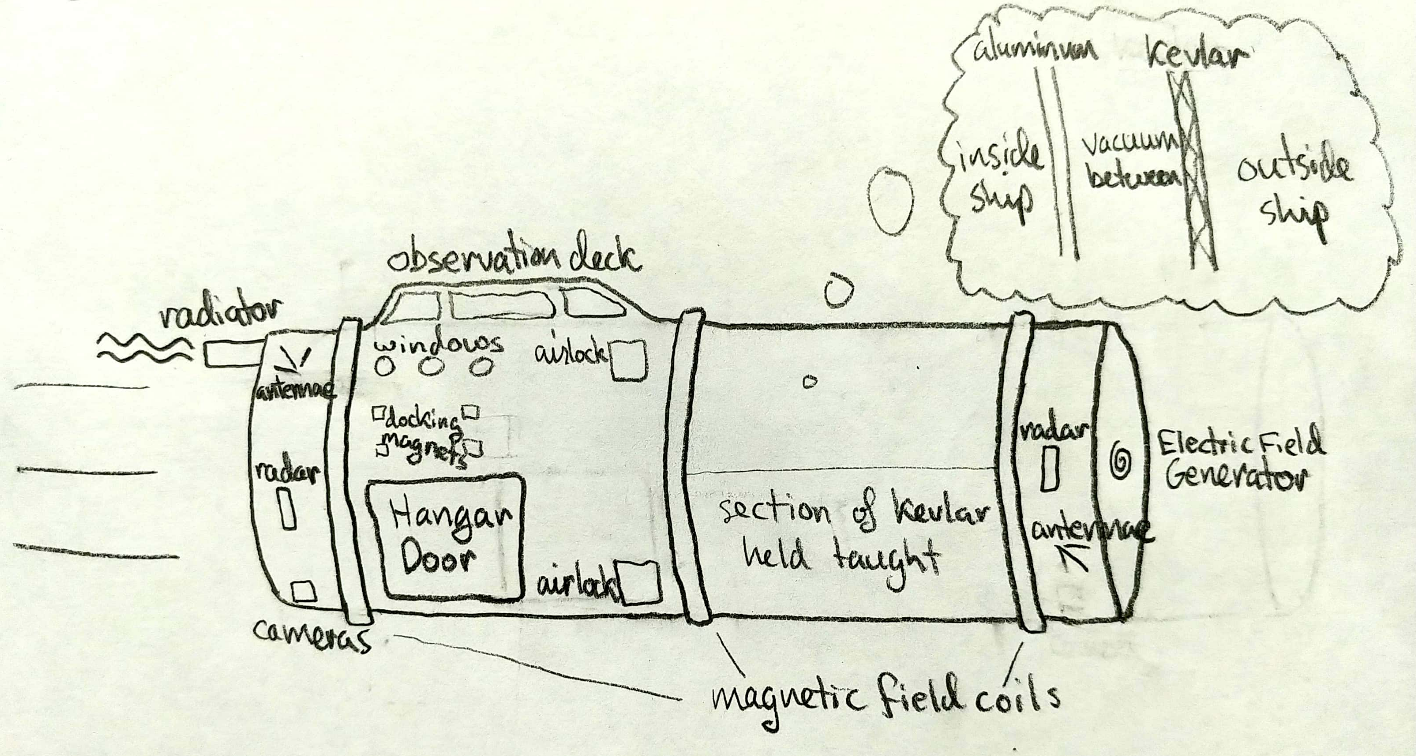
\includegraphics[scale=0.3]{Outer_Hull}

\vspace{0.3cm}
\begin{minipage}[t]{0.4\linewidth}
Fear
\begin{itemize}
\item Seeing the hull \ref{outer_hull} of a ship after a proper space combat would be unnerving to say the least. The kevlar would be spotted with huge holes that let many panels sag. Under every hole is dent after dent spotted into the aluminum plating. The sheer power of space weaponry should be awe inducing, not to mention how many shots were actually fired in a combat compared to the number of problems the players had to solve.
\end{itemize}
\end{minipage} 
\begin{minipage}[t]{0.4\linewidth}
Anger
\begin{itemize}
\item A cruel DM could keep a fighter pilot inside of the parent ship by damaging the hangar doors \ref{outer_hangar}. This could set off a chain of several failures that raise the pilot's frustration higher and higher as they simply sit there still.
\end{itemize}
\end{minipage}

\begin{minipage}[t]{0.4\linewidth}
Isolation
\begin{itemize}
\item If one of the antennae \ref{outer_antennae} are broken, it can completely disable communication either between the fighter pilot and their parent ship or between the parent ship and any backup or higher command. Leaving a ship completely in the dark is a terrifying thing, particularly for a fighter pilot completely alone in their craft. A similar feeling could also be achieved by breaking a radar dish \ref{outer_radar}. 
\end{itemize}
\end{minipage}
\begin{minipage}[t]{0.4\linewidth}
Duty
\begin{itemize}
\item If one of the doors or hatches of the hangar \ref{outer_hangar} or an airlock \ref{outer_airlocks} becomes dented, it could refuse to open, close, or lock fully. A brave soul might have to take their chances in an atmosphere that's escaping in order to physically bend the door back into a workable shape.
\end{itemize}
\end{minipage}

\vspace{0.5cm} \hspace{0.25\linewidth}
\begin{tabular}{@{} | c | l | c | @{}}
\toprule
\multicolumn{3}{|l|}{Table \ref{outer} Outer Hull Components} \\
\multicolumn{3}{|l|}{*skip nonessentials in "full table" roll} \\
\toprule
1d10 & Component & Link \\
\midrule
1 & Antennae & \ref{outer_antennae} \\
2 & Radar Dishes & \ref{outer_radar} \\
3-4 & Airlocks & \ref{outer_airlocks} \\
5-7 & Hangar Doors & \ref{outer_hangar} \\
8 & Docking Magnets & \ref{outer_docking} \\
9 & Scrap Arm & \ref{outer_arm} \\
\midrule
1d32 & Nonessentials & Link \\
\midrule
1-16 & Hull & \ref{outer_hull} \\
17-25 & Structural Beams & \ref{outer_beams} \\
26-29 & Observation Deck & \ref{outer_observation} \\
30-31 & Windows & \ref{outer_windows} \\ 
32 & Cameras & \ref{outer_cameras} \\
\bottomrule
\end{tabular}

\hspace{-18pt} \subsubsection{Antennae} \label{outer_antennae} \vspace{-0.2cm}
The ship uses various long-range antannae to communicate with nearby stations, satellites, and their own child ships. These antannae do not receive nor send signals well behind aluminum plating, meaning they cannot be inside the ship, and must be outside of the hull. They are typically hidden underneath kevlar, which does not reduce the signal nearly as much.
\\ \pbhw
{One of the metal antennae is pierced. \newline 1d2 = 1. The hole is enough to structurally compromise the antenna. See bludgeoning damage below.}
{The antenna is bent out of shape, drastically reducing its ability to detect signals in precise bandwidths. Choose either 1d2 a sending antenna or a receiving antenna. The ship can no longer send or receive messages to the following others. \newline \qthree{The ship's signal with its own children fighters is disconnected, preventing the ship from sending or receiving orders from them.}{The ship's line to the nearest station is closed, preventing the ship from receiving any new orders or guidance from command, or from requesting immediate backup.}{The ship's long-range antenna is broken, preventing them from raising concerns to higher command on the nearest planet, or receiving updates and reports from higher command.} }
{Antennae which get too hot can expand enough to receive signals at slightly the wrong frequency, and eventually a jolt can be enough to bend the wire out of shape. Then see bludgeoning damage above.}
{Stray UV light can cause voltage surges and can be enough to fry an antenna's connection. Surges typically only result in annoying blips in the signal, while the signal completely stops if the connection is fried. \newline \hspace*{3pt} Antennae are engineered to rotate when subjected to a foreign magnetic field, and when they properly align with the direction of the magnetic field, communication is still possible in both directions. On a fighter, the antennae may not be engineered this way, meaning only certain orientations will allow a fighter to communicate when under a magnetic field. Those orientations are exactly when the antenna is aligned perfectly with the magnetic field line at that point.}


\vspace{-0.5cm} \hspace{-18pt} \subsubsection{Radar Dishes} \label{outer_radar} \vspace{-0.2cm}
In order to detect nearby scrap, ships, asteroids, and other large objects, the ship employs a few sweeping radars. The radar dish uses radio waves like the antennae, which reflect off aluminum but can pass relatively unimpeded through a thin layer of kevlar, meaning it can be hidden behind the kevlar as well. 
\\ \pbhw
{A small hole is pierced in the large rotating block of metal, the head of the radar dish. Little occurs.}
{The radar head is bent out of shape significantly. \newline \qtwo{Either side of the radar is bent so far out of shape as to become useless. The head can still spin, but only one side of it can detect things.}{The entire head grinds to a halt.}}
{The metal can absorb much heat.}
{Stray UV light can cause unintended blips on the radar. \newline When right inside of a magnetic field, there is no orientation that will result in a perfect signal all the time. If you know which of the following die outcomes should occur, choose it, and if not then roll. \newline \qtwo{The current orientation allows a clear signal half of the time.}{The current orientation interferest with the signal significantly the entire time.}}


\vspace{-0.5cm} \hspace{-18pt} \subsubsection{Airlocks} \label{outer_airlocks} \vspace{-0.2cm}
The following few components will be less critical to the combat than the ones above. Only consider having an airlock break during combat if a player or NPC is inside of it.
\\ \pbhw
{The airlock is no longer airtight and will leak atmosphere while full or filling. }
{The shot collides with the airlock hatch. \newline \qtwo{The seal remains, but locking or unlocking the airlock becomes blocked by the dent.}{The dent is enough to break the seal, and atmosphere rapidly escapes.}}
{The hatch can absorb much heat, and otherwise it will go into the atmosphere.}
{Stray UV light and fast-moving microparticles can damage the seal of the airlock over time.}


\vspace{-0.5cm} \hspace{-18pt} \subsubsection{Hangar Door} \label{outer_hangar} \vspace{-0.2cm}
The hangar is a large region of the ship capable of fitting a fighter. The hangar can be pressurized so that mechanics can fix or perform maintenance on the fighter children of the ship. It then depressurizes, and its large door slide open, allowing the fighter to leave. Only consider damaging the hangar doors when somebody or something is inside of the hangar. If questioned, I would justify this by saying that problems do happen to the hangar doors (and to other less important components of the outer hull), but the problem is not significant or noteworthy if a player or object is not at risk inside, so what is the purpose of mentioning it?
\\ \pbhw
{A small hole is pierced in the enormous hangar door. Atmosphere leaks out. However, the hangar necessarily has a lot more atmosphere than most other rooms on the ship, meaning this time pressure is not as significant as other rooms.}
{The hangar door is dented. If it is closed, it is prevented from opening fully, and vice-versa.}
{The hangar door can absorb much heat, and the large atmosphere inside can absorb the rest.}
{Stray UV light and fast-moving microparticles can slowly compromise the seal of the hangar door over time.}


\vspace{-0.5cm} \hspace{-18pt} \subsubsection{Docking Magnets} \label{outer_docking} \vspace{-0.2cm}
A few permanent magnets can slide out of a container in order to attach to another piece of metal. This is used to dock the ship to a station and to dock fighters to the outside of the ship. In this state, fighter spacecraft can be ready to fly at a moment's notice, since the belly of the fighter can be opened to allow the pilot to quickly get inside while it is docked on the outside of the hull. This hatch on the fighter connects to an airlock. Again, only consider bringing up that a docking magnet has become damaged if something is attached to it.
\\ \pbhw
{A hole is pierced through the hunk of metal. Little effect.}
{The magnet is bent out of shape. \newline \qtwo{The magnet's connecting strength is reduced, so it becomes easy for something to knock it off.}{The magnet can no longer connect at all.}}
{The hunks of metal absorb much heat.}
{Stray UV light and microparticles do little as they act like piercing damage in certain ways. \newline A docking magnet encountering another strong magnetic field can weaken the magnet if it is pointed against the docking magnet or strengthen it if they are pointed in the same direction. Typically this will only weaken the magnet over time, therefore requiring frequent replacement.}


\vspace{-0.5cm} \hspace{-18pt} \subsubsection{Scrap Arm} \label{outer_arm} \vspace{-0.2cm}
This arm is a small prehensile robotic arm with both an electromagnet and grabbing fingers attached to the end. It is used to pick out important pieces of scrap or for other miscellaneous uses. Only consider damaging this arm if it is being used to grab something.
\\ \pbhw
{\qtwo{A metal arm is pierced, doing little.}{A hydraulic tube is pierced. One joint of the arm no longer can rotate back and forth, as hydraulic fluid spills out.}}
{One section of the arm is bent out of shape. \newline \hspace{3pt} 1d2 = 1. The hit also disconnects or damages one of the pneumatic pipes, spilling hydraulic fluid and stopping one joint of the arm from working.}
{The metal of the arms absorb all the heat.}
{UV light and microparticles are particularly dangerous for such a delicately-controlled system. It can damage the metal joints over time. The seals of the hydraulic system can also become compromised. Fast-moving microparticles can also pierce large enough holes to leak hydraulic fluid itself. \newline \hspace*{3pt} Under a strong magnetic field, the arm will move in strange directions and will be very difficult to control.}


\vspace{-0.5cm} \hspace{-18pt} \subsubsection{Hull} \label{outer_hull} \vspace{-0.2cm}
The hull of the ship is composed of two layers. The first layer is a sheet of dense kevlar \cite{kevlar_properties}. This layer obliterates railgun flak shots when they arrive. This obliteration scatters the shot so that it hits a wider area of the hull underneath, and therefore the dent will be wider but more shallow, and is much less likely to pierce the hull. Below the kevlar the proper hull is a thin sheet of aluminum, reinforced by its precisely-engineered shape that maintains structural integrity while saving mass.
\\ \pbhw
{The piercing shots of a ray accelerator essentially go straight through the relatively thin kevlar and aluminum layers. The shot will continue until it encounters enough different layers of metal, or it will stop immediately if it hits a vat of liquid.}
{The railgun shot is shattered by the kevlar layer and spreads its energy over a larger area. Once the kevlar is hit like this, it becomes much weaker and is no longer held taught. If a railgun shot hits the same place again, it the kevlar will deflect it directly into the dent that was just made, and it can pierce through the aluminum. Once this happens, the shot continues until it hits a hunk of metal and it severely dents that. The shot may bounce and hit other nearby parts. The hole in the aluminum hull is ragged and difficult to achieve a proper seal around.}
{Kevlar absorbs much heat, and if you can get it hot enough it will decompose and become weaker. After that, some heat may transfer to the aluminum plate, which spreads heat very quickly and will only melt at extreme temperatures. In short, the hull is affected by heat very little.}
{Repeated exposure to UV radiation noticeably decomposes the kevlar outer layer of the hull. It is also designed to shatter microparticles, stopping them from piercing the hull while damaging and weakening the kevlar. }


\vspace{-0.5cm} \hspace{-18pt} \subsubsection{Structural Beams} \label{outer_beams} \vspace{-0.2cm}
A few other components of the ship stick out of the hull, including the radiator and engine exhaust vent. The structural beams of the ship hold the large magnetic field coils \ref{grid_m_field_coils}. Evenly spaced along the length of the ship are these beams, which separate sections of kevlar held taught. 
\\ \pbhw
{Adds some slight wear to the beam.}
{A structural beam taking a direct hit from a railgun is not a good thing. The beam becomes dented and its structure is compromised. Every time that the ship goes to full acceleration while it is still dented and compromised, roll 1d2. On 1d2 = 1, the force is enough to warp the entire structure of the ship. The long cylindrical ship now is slightly bent at this beam. Firing the engine now causes the entire ship to spin, and some rooms may crack open to the vacuum of space.}
{The huge metal beams absorb heat well.}
{UV radiation wears away at the beams over time. The beams at the rear of the ship become worn by constantly being pushed strongly by the engine. }


\vspace{-0.5cm} \hspace{-18pt} \subsubsection{Observation Deck} \label{outer_observation} \vspace{-0.2cm}
The ship has a room with a series of windows that can look in many directions. Only considering damaging this room if something or somebody is inside of it.
\\ \pbhw
{A small hole is pierced through a window. \newline 1d4 = 1. Cracks form, and the pressure of the atmosphere is enough to blow the window out. See bludgeoning damage below.}
{The railgun shot completely shatters the window, instantly sucking out the entirety of the atmosphere.}
{The glass does not fare well to repeated or sudden heating.}
{The glass and seals between panes slowly decompose from UV radiation. Microparticles can puncture microscopic holes in a window that can still leak atmosphere.}


\vspace{-0.5cm} \hspace{-18pt} \subsubsection{Windows} \label{outer_windows} \vspace{-0.2cm}
Around the ship are various small, circular, thick-paned windows for crew to look out.
\\ \pbhw
{The window has a hole in it. \newline 1d4 = 1. Cracks form and the pressure is enough to shatter the window. See bludgeoning damage below.}
{The majority of the window shatters, letting out atmosphere extremely quickly.}
{The glass does not appreciate repeated or sudden heating.}
{The glass and seal slowly decompose from UV radiation. Microparticles can puncture microscopic holes in a window that can still leak atmosphere.}


\vspace{-0.5cm} \hspace{-18pt} \subsubsection{Cameras} \label{outer_cameras} \vspace{-0.2cm}
Various cameras of several wavelengths of light are placed around the outer hull of the ship so that the the full battlefield can be displayed for the commanders inside.
\\ \pbhw
{\qtwo{A part of the electronics of the camera is pierced through, completely disabling it.}{The lens chamber is pierced, allowing in extra light.}}
{One of the cameras is smashed to pieces.}
{The intricate electronics of a camera's optical sensor will be the first to melt, followed by the rest of the circuitry.}
{Cameras in space are subject to harmful radiation. Stray UV photons fry individual pixels of the optical sensor over time. Those same photons can interfere with wiring as well and cause errors in the electronics of the camera. Cameras have some shielding but this is still not enough.}

\begin{comment}
\subsection{Blank System} \label{blank}

System description

\vspace{0.3cm}
\begin{minipage}[t]{0.4\linewidth}
Fear
\begin{itemize}
\item problem
\end{itemize}
\end{minipage} 
\begin{minipage}[t]{0.4\linewidth}
Anger
\begin{itemize}
\item problem
\end{itemize}
\end{minipage}

\begin{minipage}[t]{0.4\linewidth}
Isolation
\begin{itemize}
\item problem
\end{itemize}
\end{minipage}
\begin{minipage}[t]{0.4\linewidth}
Duty
\begin{itemize}
\item problem
\end{itemize}
\end{minipage}

\vspace{0.5cm} \hspace{0.25\linewidth}
\begin{tabular}{@{} | c | l | c | @{}}
\toprule
\multicolumn{3}{|l|}{Table \ref{blank} Blank Components} \\
\toprule
1d?? & Component & Link \\
\midrule
1 & Blank Component & \ref{blank_component} \\
2 & Blank Component 2 & \ref{blank_component2} \\
\bottomrule
\end{tabular}

\hspace{-18pt} \subsubsection{Blank Component} \label{blank_component} \vspace{-0.2cm}
Component description
\\ \pbhw
{}
{}
{}
{}

\vspace{-0.5cm} \hspace{-18pt} \subsubsection{Blank Component 2} \label{blank_component2} \vspace{-0.2cm}
Component description
\\ \pbhw
{}
{}
{}
{}

\end{comment}


\newpage

\section{Combats} \label{combats}

Combats 1-4 have a questline included in them in section \ref{quests}, while combats 5-8 are more general, late game combats that can be used to either extend the length of an existing campaign or offer endgame combats to play through after the story is finished.

\subsection{Combat 1: Formula S Track} \label{combat_1}

This combat takes place in a location related to the quests included later in the document. In practice, you can take this combat and use it in any other location (near a station) with little problem, as long as you change the reason for engagement.

\begin{minipage}[t]{0.5\linewidth}
\begin{tabular}[t]{| p{7cm} |}
\toprule
\multicolumn{1}{|c|}{Combat Description} \\
\midrule
Simultaneous Problems :- \\
Only one problem at a time. \\	
\midrule
Component Complexity :- \\
Start the combat by rolling once for each player. Roll on only the bottom half of the system's table to ensure the component is rather simple. Then, you can optionally continue the combat as long as you want by rolling on the entire system table for up to each player again. \\
\midrule
Problem Complexity :- \\
Ensure the problem only affects a single component at a time. \\
\midrule
Enemy Description :- \\
Two fighter spacecraft lurking behind a beacon that marks a corner in the racetrack. \\
\midrule
Reason for Engagement :- \\
The fighters are shooting at the racers. Even shooting close to a racer will trigger the racer's automatic dodging system, which can knock them off course enough to change the outcome of a race. Unfortunately, one of the shot hits one of the racers, and hard. The enemy fighters immediately run. \\
\bottomrule
\end{tabular}
\end{minipage}
\begin{minipage}[t]{0.45\linewidth}
\begin{tabular}[t]{| r | p{5cm} |}
\toprule
\multicolumn{2}{| c |}{Battlefield Description} \\
\midrule
location & Formula S track. Fighter spacecraft have been modified to be agile racing ships, which are currently in a race right next to a space station. \\
distances & The enemy spacecraft begin in close range but immediately run away. They turn and take four shots while in medium range before running again. \\
comm.s time & Instant communication with the station and the planet below. \\
\begin{tabular}[c]{@{}r@{}}relative\\velocities\end{tabular} & All begin stationary. \\ 
visibility & Racers and enemies fully lit by sun. \\ 
ions & none \\
radioactivity & none \\
UV radiation & Full view of sun. \\
molecules & Stray O$_2$(g), N$_2$(g), and H$_2$O(g) from station. \\
scrap & A few nuts and bolts from the station. \\
asteroids & none \\
\bottomrule
\end{tabular}
\end{minipage}

\newpage
\subsection{Combat 2: Industrial District} \label{combat_2}
The ship takes a detour above the factories and plants as they leave the station. The station is composed of the commercial and residential districts, spinning on the outside of a ring as to have gravity, while the industrial district and docks are floating in zero gravity next to the station. The industrial district is situated a ways away from the station to avoid debris contamination.

\begin{minipage}[t]{0.5\linewidth}
\begin{tabular}[t]{| p{7cm} |}
\toprule
\multicolumn{1}{|c|}{Combat Description} \\
\midrule
Simultaneous Problems :- \\
Keep the focus on one problem at a time. However, ensure that the problem has adequate pressure. If something intense like liquid nitrogen escapes, that has enough time pressure in the form of the encroaching cold. If something simple happens, like a water tank getting pierced, that problem has no pressure on it whatsoever. For a simple problem like that, mention right away that a wall was also pierced, so that the time pressure of the atmosphere escaping is put on the player. \\	
\midrule
Component Complexity :- \\
Roll on the full table like an adult. Remember to put pressure on, particularly if your roll ends up being in the bottom half of the table. \\
\midrule
Problem Complexity :- \\
Keep the problems still isolated to one component at a time. If you end up rolling a problem that seems too easy for a player, then consider having it affect a more complicated part nearby to make sure they are working on the top half of the table. \\
\midrule
Enemy Description :- \\
The ships in the graveyard are as large as the players' ship. As the players fly over, it turns out that the radiator is blaring. \\
\midrule
Reason for Engagement :- \\
The heat from the radiator hits the players' ship, immediately setting off alarms. This is how the players learn the ship is crewed. The people here are running a ship without license or paying proper tariffs, in order to make ice and illegally sell it on the station. \\
\bottomrule
\end{tabular}
\end{minipage}
\begin{minipage}[t]{0.45\linewidth}
\begin{tabular}[t]{| r | p{5cm} |}
\toprule
\multicolumn{2}{| c |}{Battlefield Description} \\
\midrule
location & Above the station's industrial district. Directly above a graveyard of large ships, turned vertical.  \\
distances & Begin right above one of the ships in the graveyard, in close range. \\
comm.s time & Fractions of a second. \\
\begin{tabular}[c]{@{}r@{}}relative\\velocities\end{tabular} & Moving past the ship graveyard, while the ships in it are stationary. \\ 
visibility & The enemy ship is in the shadow of a few other ships in the graveyard, so that less than a quarter of it is in sunlight. \\ 
ions & Light industrial debris. Solar wind. \\
radioactivity & Light industrial byproduct. \\
UV radiation & Sunlight. \\
molecules & Light industrial debris in the form of mostly atmospheric gases. \\
scrap & Industrial scrap still floats around from various accidents. \\
asteroids & none \\
\bottomrule
\end{tabular}
\end{minipage}

\newpage
\subsection{Combat 3: Derelict Satellite} \label{combat_3}

The players' ship happens to be passing by an old satellite, in a low orbit around the planet. These satellites are old enough to be outfitted with extremely light thermoelectric generators which would be perfect for a racing spacecraft.

\begin{minipage}[t]{0.5\linewidth}
\begin{tabular}[t]{| p{7cm} |}
\toprule
\multicolumn{1}{|c|}{Combat Description} \\
\midrule
Simultaneous Problems :- \\
Now is the time to present each player with simultaneous problems if they have not had one already. Have the piercing shot go through two systems, or the bludgeoning shot bounce. \\	
\midrule
Component Complexity :- \\
Roll on both halves of the table for the first problem, and on the bottom half for any additional problems. \\
\midrule
Problem Complexity :- \\
Again keep the problems focused on one system. If two simultaneous problems end up being adjacent, and the player is up to the challenge, then consider having the problems affect each other. \\
\midrule
Enemy Description :- \\
A swarm of unmanned drone spacecraft still remain around the satellite. They are technically illegally guarding the satellite, as salvagers should have come by now, but the government/corporation that set up the satellite no longer exists. \\
\midrule
Reason for Engagement :- \\
The drones will attack any spacecraft that tries to get near to the satellite. Luckily they die in one hit almost every time. \\
\bottomrule
\end{tabular}
\end{minipage}
\begin{minipage}[t]{0.45\linewidth}
\begin{tabular}[t]{| r | p{5cm} |}
\toprule
\multicolumn{2}{| c |}{Battlefield Description} \\
\midrule
location & Low orbit near a derelict satellite. \\
distances & Long range to the satellite, medium range to the drones. Can approach from as far away, and as slowly, as the players want. \\
comm.s time & Several seconds to the station. \\
\begin{tabular}[c]{@{}r@{}}relative\\velocities\end{tabular} & Likely with slight forward velocity compared to a stationary satellite. \\ 
visibility & Lit by sun. \\ 
ions & Light amounts of upper atmosphere are ionized by the sunlight. \\
radioactivity & The reactor inside the satellite is still noticeably radioactive. Enough to damage a system when close range to the satellite. When medium range, light but detectable radiation. \\
UV radiation & Sunlight. \\
molecules & Light upper atmosphere. \\
scrap & Many various parts of the satellite have broken and drifted off. Surrounded by a blob of metal scrap. \\
asteroids & none  \\
\bottomrule
\end{tabular}
\end{minipage}

\newpage
\subsection{Combat 4: In the Shadow of the Station} \label{combat_4}

The players are returning from a week on patrol and encounter some fishy ships right next to the station.

\begin{minipage}[t]{0.5\linewidth}
\begin{tabular}[t]{| p{7cm} |}
\toprule
\multicolumn{1}{|c|}{Combat Description} \\
\midrule
Simultaneous Problems :- \\
One or more at a time. \\
\\	
\midrule
Component Complexity :- \\
Begin with one component in the top half, and all problems afterwards roll on the bottom half. \\
\midrule
Problem Complexity :- \\
Step it up! Have one of the bottom half problems affect a nearby complex component. \\
\midrule
Enemy Description :- \\
One large ship with a few fighters. \\
\midrule
Reason for Engagement :- \\
The enemies are blasting open the side of the space station. This room is storing the ice that will be used as fuel by one of the racers for quest for \ref{quest_4}. \\
\bottomrule
\end{tabular}
\end{minipage}
\begin{minipage}[t]{0.45\linewidth}
\begin{tabular}[t]{| r | p{5cm} |}
\toprule
\multicolumn{2}{| c |}{Battlefield Description} \\
\midrule
location & Immediately next to the side of the rotating part of the station. \\
distances & Approach from as far away as desired. \\
comm.s time & Instant. \\
\begin{tabular}[c]{@{}r@{}}relative\\velocities\end{tabular} & Enemies stationary, player approaching.\\ 
visibility & Within the shadow of the station. \\ 
ions & none \\
radioactivity & none \\
UV radiation &  none \\
molecules & Enemies opening the walls of the station, letting out atmosphere. \\
scrap & Tools and scrap from the damaged walls floats out. \\
asteroids & Chunks of ice of all sizes are floating out of the room in the station with the damaged walls, a large cargo bay. \\
\bottomrule
\end{tabular}
\end{minipage}

\newpage
\subsection{Combat 5: Behind a Faraway Moon} \label{combat_5}

All combats from now on will not be part of the main questline described in the next section. These are standalone combats that you can use as a part of your story, or use if your players want to keep playing through combats after the story.

This combat is an ambush in the shadow of a moon. The players' ship decides to take a transfer with another sister ship, and they encounter two other ships in the darkness of the moon.

\begin{minipage}[t]{0.5\linewidth}
\begin{tabular}[t]{| p{7cm} |}
\toprule
\multicolumn{1}{|c|}{Combat Description} \\
\midrule
Simultaneous Problems :- \\
One or more at a time. \\	
\midrule
Component Complexity :- \\
Roll anywhere on the table. \\
\midrule
Problem Complexity :- \\
If a problem is on the bottom half of the table, have it then affect a nearby complex component. \\
\midrule
Enemy Description :- \\
Two large ships appear from around the moon. \\
\midrule
Reason for Engagement :- \\
The enemies only expected one police vessel to take this transfer orbit, but the players' ship decided to join the transfer as well. \\
\bottomrule
\end{tabular}
\end{minipage}
\begin{minipage}[t]{0.45\linewidth}
\begin{tabular}[t]{| r | p{5cm} |}
\toprule
\multicolumn{2}{| c |}{Battlefield Description} \\
\midrule
location & In the shadow of the moon of a different planet than the one that the station orbits. \\
distances & Long range which rapidly becomes close. \\
comm.s time & Anywhere from 5 minutes to an hour (~ 3 x 1d20 minutes). \\
\begin{tabular}[c]{@{}r@{}}relative\\velocities\end{tabular} & The enemies are orbiting in the opposite direction as the friendly ships around the moon. The ships will become close quickly and will pass each other at huge speeds. \\ 
visibility & Complete darkness. \\ 
ions & none \\
radioactivity & none \\
UV radiation & none \\
molecules & none \\
scrap & none \\
asteroids & none \\
\bottomrule
\end{tabular}
\end{minipage}

\subsection{Combat 6: A Station} \label{combat_6}

\begin{minipage}[t]{0.5\linewidth}
\begin{tabular}[t]{| p{7cm} |}
\toprule
\multicolumn{1}{|c|}{Combat Description} \\
\midrule
Simultaneous Problems :- \\
One cascade at a time. \\	
\midrule
Component Complexity :- \\
Roll on the top half of the table to begin.\\
\midrule
Problem Complexity :- \\
Propagate the problem to as many different systems as you can. The goal of this combat is not to destroy an entire station, but to escape. This sort of combat lends itself to the most intense kinds of problems, problem cascades. \\
\midrule
Enemy Description :- \\
A small rotating space station set up to oversee some mining and industrial operations nearby. If the players manage to disable one weapon on the space station, it quickly rotates so that the next weapon down will take its place. \\
\midrule
Reason for Engagement :- \\
In the context of the quests included, this station could be a base of operations for questionable ice or rocketry production that the players are investigating. \\
\bottomrule
\end{tabular}
\end{minipage}
\begin{minipage}[t]{0.45\linewidth}
\begin{tabular}[t]{| r | p{5cm} |}
\toprule
\multicolumn{2}{| c |}{Battlefield Description} \\
\midrule
location & Near a space station. \\
distances & Medium range to it. \\
comm.s time & Between 5 min and an hour to home station. Optionally the enemy station can be the player's home station. \\
\begin{tabular}[c]{@{}r@{}}relative\\velocities\end{tabular} & Almost nothing. \\ 
visibility & Station half lit by sun. \\ 
ions & Stray ions from industrial activity nearby. \\
radioactivity & none \\
UV radiation & Sunlight. \\
molecules & Stray dust from industrial activity nearby. \\
scrap & none \\
asteroids & Rare small asteroid. \\
\bottomrule
\end{tabular}
\end{minipage}

\newpage
\subsection{Combat 7: Trained Fighter Squadron} \label{combat_7}

\begin{minipage}[t]{0.5\linewidth}
\begin{tabular}[t]{| p{7cm} |}
\toprule
\multicolumn{1}{|c|}{Combat Description} \\
\midrule
Simultaneous Problems :- \\
One or more at a time. \\	
\midrule
Component Complexity :- \\
Roll anywhere on the table. \\
\midrule
Problem Complexity :- \\
If a problem is on the bottom half of the table, have it then affect a nearby complex component. \\
\midrule
Enemy Description :- \\
A small group (4-5) of highly trained fighter pilots engages the player's ship from an asteroid field. \\
\midrule
Reason for Engagement :- \\
In the context of the quests provided, these fighters could be the same ones trying to alter the outcome of every race. They would likely have allegiance to either the glacier or brazier racer.\\
\bottomrule
\end{tabular}
\end{minipage}
\begin{minipage}[t]{0.45\linewidth}
\begin{tabular}[t]{| r | p{5cm} |}
\toprule
\multicolumn{2}{| c |}{Battlefield Description} \\
\midrule
location & Inside of an asteroid field. \\
distances & Enemies use asteroids to sneak into medium range without being seen before engaging. \\
comm.s time & Between 5 minutes and an hour from the home station. \\
\begin{tabular}[c]{@{}r@{}}relative\\velocities\end{tabular} & Players' ship moving forward over the field, the fighters stationary inside of it. \\ 
visibility & The sun illuminates every asteroid, though the fighters are good at staying in shadow. \\ 
ions & none \\
radioactivity & none \\
UV radiation & Sunlight. \\
molecules & Light dust. \\
scrap & Small pebbles. \\
asteroids & Numerous asteroids of all sizes. \\
\bottomrule
\end{tabular}
\end{minipage}

\subsection{Combat 8: An Entire Planet} \label{combat_8}

Whenever a ballistic missile fired from the planet takes a railgun or ray shot, \newline \qeq{1d4}{1-2.}{The hole or dent does little to nothing.}{3.}{The hole or dent disables the targeting and guidance systems, killing it quietly.}{4.}{The hole or dent sets off the ignition system, instantly exploding the rocket.}{}{}

\begin{minipage}[t]{0.5\linewidth}
\begin{tabular}[t]{| p{7cm} |}
\toprule
\multicolumn{1}{|c|}{Combat Description} \\
\midrule
Simultaneous Problems :- \\
One cascade at a time. \\	
\midrule
Component Complexity :- \\
Roll on the top half of the table to begin. \\
\midrule
Problem Complexity :- \\
Propagate the problem to as many different systems as you can. The goal of this combat is not to destroy an entire planet, but to escape. This sort of combat lends itself to the most intense kinds of problems, problem cascades. \\
\midrule
Enemy Description :- \\
The player's home station has identified them as a threat. The home station fires weaponry which causes most of the problems, while the entire planet below launches its defenses. These planetary defenses include only missiles. \\
\midrule
Reason for Engagement :- \\
The home station and planet could be on high alert for the players' ship because it engaged a station in combat 6 \ref{combat_6}. \\
\bottomrule
\end{tabular}
\end{minipage}
\begin{minipage}[t]{0.45\linewidth}
\begin{tabular}[t]{| r | p{5cm} |}
\toprule
\multicolumn{2}{| c |}{Battlefield Description} \\
\midrule
location & Nearby the players' home station. \\
distances & Medium range from the station. \\
comm.s time & Instantaneous. \\
\begin{tabular}[c]{@{}r@{}}relative\\velocities\end{tabular} & Players moving slightly towards the station. \\ 
visibility & Fully lit by sun. \\ 
ions & none \\
radioactivity & none \\
UV radiation & Sunlight. \\
molecules & Chemical waste from exploded rockets. \\
scrap & Physical waste from exploded rockets. \\
asteroids & Large rockets that are dead in the air. \\
\bottomrule
\end{tabular}
\end{minipage}

\begin{comment}
\newpage
\subsection{Combat N: Blank Combat} \label{combat_n}

\begin{minipage}[t]{0.5\linewidth}
\begin{tabular}[t]{| p{7cm} |}
\toprule
\multicolumn{1}{|c|}{Combat Description} \\
\midrule
Simultaneous Problems :- \\
\\	
\midrule
Component Complexity :- \\
\\
\midrule
Problem Complexity :- \\
\\
\midrule
Enemy Description :- \\
\\
\midrule
Reason for Engagement :- \\
\\
\bottomrule
\end{tabular}
\end{minipage}
\begin{minipage}[t]{0.45\linewidth}
\begin{tabular}[t]{| r | p{5cm} |}
\toprule
\multicolumn{2}{| c |}{Battlefield Description} \\
\midrule
location &  \\
distances & \\
comm.s time & \\
\begin{tabular}[c]{@{}r@{}}relative\\velocities\end{tabular} & \\ 
visibility & \\ 
ions & \\
radioactivity & \\
UV radiation &  \\
molecules &  \\
scrap &  \\
asteroids &  \\
\bottomrule
\end{tabular}
\end{minipage}
\end{comment}



\newpage
\section{Quests} \label{quests}

The following few quests is an example of how you can guide your players through building their own spaceship. The quests will take the players through three locations with various hazards, including the outside of a large destroyed ship, the inside of such a ship, and nearby to a derelict satellite. These allow the players to pick up a fighter ship hull, radiator, and reactor. 

If you want to create your own quest involving the players building their own ship, you can still find inspiration below. You can include more different systems of the ship than just the reactor and radiator that the player must scavenge. Additionally, the locations described in each quest have hazard tables which can be applicable to surprisingly many different situations. 

\subsection{Quest 1: Retrieving a Hull} \label{quest_1}

Today is a big day. The major local space station has organized a display, and has invited the policemen to join when they are not overseeing the events. The events will include space skating, a Formula S race, and a weaponry test.

The crew is allowed to watch the pleasant display of space skating outside the window of the station's main, high-class observation deck. It is zero-g, but drinks are available in pouches. This is a fine time to introduce the player's characters to each other, if it hasn't happened already.

Then the crew boards and is required to keep watch over the Formula S game, where the fastest and most maneuverable spaceships gather each year to race. Combat 1 occurs \ref{combat_1}. The crew is allowed back onto the station as proper repair crews rush in. Over the loudspeaker they hear that the Formula S race is officially postponed to a later date due to excess scrap metal on the runway.  Then they hear that one of the teams has dropped out of the race due to loss of equipment (if players ask, the reactor was smashed, fighter completely irradiated, unusable). 

When the players sit down for drinks to watch the weaponry test, the barkeep points out that new teams are allowed to sign up for the race. He then offers that he knows where to get a free ship. Make sure the players get the hint that this is the main quest. The players should feel proud for having the bravery to sign up and excited for what is to come. That is, until the barkeep then points out that their "free ship" is inside the hangar of a large ship. And that ship is about to be destroyed as part of the weaponry test.

The players will have to put on EV suits (optionally the fighter pilot may fly their spacecraft) and retrieve the fighter from the hangar of the larger ship. They can either choose to do this during the weaponry test, in which case railguns will be constantly firing, or to wait until after the weaponry test when things are safer. Both options come with similar but separate dangers and hazards, listed in the tables below.

\begin{minipage}[t]{0.45\linewidth}
\begin{tabular}[t]{| c | p{5 cm} |}
\toprule
\multicolumn{2}{| l |}{Table \ref{quest_1}.1 During Weaponry Test} \\
\midrule
1d8 & Hazard \\
\midrule
1 & One of the glass windows is shattered right in front of the eyes of the player. Glass scatters and may puncture their suit. \\
2 & The tools and scrap of a room are suddenly vented from the ship. These nuts, bolts, and wrenches can get moving quickly, and can hurt. \\
3 & Hot gas is escaping from the ship, or a gas is being heated by the radiator. \\
4 & Cold gas is escaping. \\
5 & A radiator is blaring heat in the way. \\
6 & Stray hunks of metal shoot off in random direction and can get in the way. \\ 
7 & Wiring on the ship is exposed and generating sparks that leap to nearby things. \\
8 & The ship's strong magnetic fields can get in the way of moving a fighter ship or can send other debris scattering in strange directions. \\
\bottomrule
\end{tabular}
\end{minipage}
\begin{minipage}[t]{0.45\linewidth}
\begin{tabular}[t]{| c | p{6cm} |}
\toprule
\multicolumn{2}{| l |}{Table \ref{quest_1}.2 After Weaponry Test} \\
\midrule
1d6 & Hazard \\
\midrule
1 & A large section of windows has broken and the cloud of shattered glass is in the way. \\
2 & A room is open to space, and has evacuated the tools and other things inside. These are now scattered in a cloud of scrap. \\
3 & One of the hot gases has escaped and has kept its heat. Otherwise a gas has escaped and was heated by either the radiator or the sun. \\
4 & A cold gas has escaped and has remained in shadow in order to retain its coldness.  \\
5 & A designated crew in EV suits and salvaging frigates has purchased the rights to scavenge this vessel. Their large magnetic arms can lock onto the fighter and hold it in place. \\
6 & A scientific crew has also went in, and is interested in pieces of metal that have been impacted or pierced. One wing of the fighters hull is damaged, and the scientists kindly ask for it. If given, the players will have to find a new piece of metal for that hull. \\
\bottomrule
\end{tabular}
\end{minipage}

\vspace{0.2cm}
Once the fighter spaceship has been retrieved, the ship will be missing several key components. It has been stripped of its radiator, reactor, and railgun due to their complexity and expensiveness, while the engine remains. If the players waited until after the weaponry test to retrieve it, the ship will have a total of 1d4 severe dents in its hull and its glass window(s) will be shattered. You can roleplay that other random things are missing like radios and communication devices, but the only parts truly necessary to make this ship flyable are a radiator, reactor, and to fix the hull if it's damaged. 

This quest leads into the four other quests. Two of these will be to retrieve a free radiator and reactor from dangerous places, and the other two are the warmup laps and race. 

\subsection{Quest 2: Retrieving a Radiator} \label{quest_2}

This quest involves navigating a large ship that has recently been destroyed in combat. Included is a table in which you can roll to determine the hazards in a series of rooms as the players navigate the ship. 

This quest takes place immediately after combat 2 \ref{combat_2}. The combat involves disabling or one large enemy ship. Once it is disabled, I expect the players will want to board the ship to arrest the crew. The real purpose of them entering the ship is to salvage a radiator from the ship. Either way, they will traverse the inside of a dying ship room by room.

\begin{tabular}[t]{| c | p{12.5cm} |}
\toprule
\multicolumn{2}{|l|}{Table \ref{quest_2} Navigating a Large Dying Ship} \\
\midrule
1d8 & Hazard in Room \\
\midrule
1 & The room stored liquid nitrogen for either the atmosphere, RCS, or thermal systems. This nitrogen has leaked everywhere in the room and by now has mostly evaporated into thick clouds. The oxygen content of the room is significantly lowered. Additionally, the main concern is that everything in the room has a layer of frost on it from the freezing nitrogen. The handle of the next door is frozen shut, and it is brittle enough that hitting it hard would break it off. \\
2 & The room contains a radiator. Several other chambers for life support are also in the room, due to the hot temperatures required for the chemistry. The heat from these and the radiator has brought the room to a near-boiling temperature. Staying in the room for too long will cause heatstroke, and the door handles are too hot to touch. \\
3 & The room contains the thick wiring needed to deliver power either from the reactor or to a railgun, ray accelerator, or magnetic field coil. This wiring has been smashed or pierced, and is sparking everything nearby. This can either block a doorway or some frightened crew members. \\
4 & The room used to contain a storage vat of hydrogen for either the engine or life support systems. This hydrogen has leaked out and boiled to fill the room. As soon as the door is opened to this room, hydrogen gas completely surrounds the players. The slightest spark between two metals, the slightest surge in an electronic device, or a single very rapid, jarring movement can set the entire room alight. \\
5 & The room is mostly undamaged but the jerks and accelerations from combat have thrown various tools and such around the room. Consider having this happen in a room with a railgun, so that hunks of railgun ammo are floating everywhere, or in a mechanics bay so that various wrenches, hammers, and other tools are flying around everywhere. \\
6 & The room is mostly undamaged but a stray shot has shattered a glass window. Consider having this occur in an observation deck, so that several series of windows right next to each other can be shattered. \\
7 & The room contains around half of the crew, who simply ask for passage aboard the players' ship for their own safety. \\
8 & The room is a cargo bay where the crew stores the ice that they make. Crew members are currently stuffing ice into an airlock to vent it to space. When they see the players, they immediately close and vent the airlock, and then some of them stop while perhaps one or two run. \\
\bottomrule
\end{tabular}

\subsection{Quest 3: Navigating a Broken Satellite} \label{quest_3}

The following quest involves the players trying to retrieve a piece of equipment from an old broken satellite. The table of hazards is similar to the outside of a larger spaceship, but involves smaller components as well. 

This quest happens directly after combat 3 \ref{combat_3}. The players have all the time in the world to get past these hazards.

\begin{tabular}[t]{| c | p{12.5cm} |}
\toprule
\multicolumn{2}{|l|}{Table \ref{quest_3} Navigating a Broken Satellite} \\
\midrule
1d8 & Hazard around satellite \\
\midrule
1 & A layer of fine, thin pieces of metal hovers around the satellite. EV suits passing through have a risk of being punctured. \\
2 & A few huge chunks of metal have broken off the satellite and are blocking the way. \\
3 & Some pieces of scrap have accumulated a strong amount of charge. Coming near them may cause shocks. \\
4 & Large thin pieces of foil that used to surround the satellite have now fluttered off, and have absorbed huge amounts of heat from the sun. Touching one will sear it onto whatever it touches. \\
5 & A few pieces of the metal chamber of the reactor were rusted off and now float, still irradiated, near the satellite. As a DM, dare not ever let a player touch one of these, and always make sure they know the dangers of radioactivity. \\
6 & A solar panel has shattered and its pieces are numerous and pointy. Can cause puncturing. \\
7 & The thin metal sheets of the radiator now fly about. They both absorb a huge amount of heat from the sun and are very sharp. \\
8 & A few pieces of the antennae have broken off, and their pointy ends now spin around near the satellite. \\
\bottomrule
\end{tabular}

\vspace{0.2cm}
Once the players reach the satellite itself, a few things will be wrong with the reactor. The reactor will be open on one side, so have the players find a new thick piece of metal to be a new wall. The reactor will be welded to the rest of the satellite, so either let them bring the entire satellite into the ship's hangar or let them cut it out of the satellite.

\subsection{Quest 4: The Race} \label{quest_4}

After combat 4 \ref{combat_4} and some shore leave, the day of the race comes. The race will focus on three specific racers: the players, a racer who uses ice as fuel (the "glacier racer"), and a racer who uses solid rockets as fuel (the "brazier racer"). Feel free to use proper names instead. 

The warmup lap takes place a few hours before the race itself. Let the players show off during the warmup lap and use as much as fuel as they want. The glacier racer will use a ton of fuel to do spirals, backflips, and other crazy maneuvers. The brazier racer will be more conservative with fuel but will launch fireworks and sparklers (fairly, not interrupting anything). 

At the end of the warmup lap, have two more fighters appear and try to fire at the buoys that mark the racetrack. But instead of a proper combat, simply let the players' ship (without them on it) and a few other police vessels smash them to pieces. Then let a few hours pass as the racetrack is cleaned up, and optionally allow the players to interact with the other racers before the race.

\vspace{0.2cm}
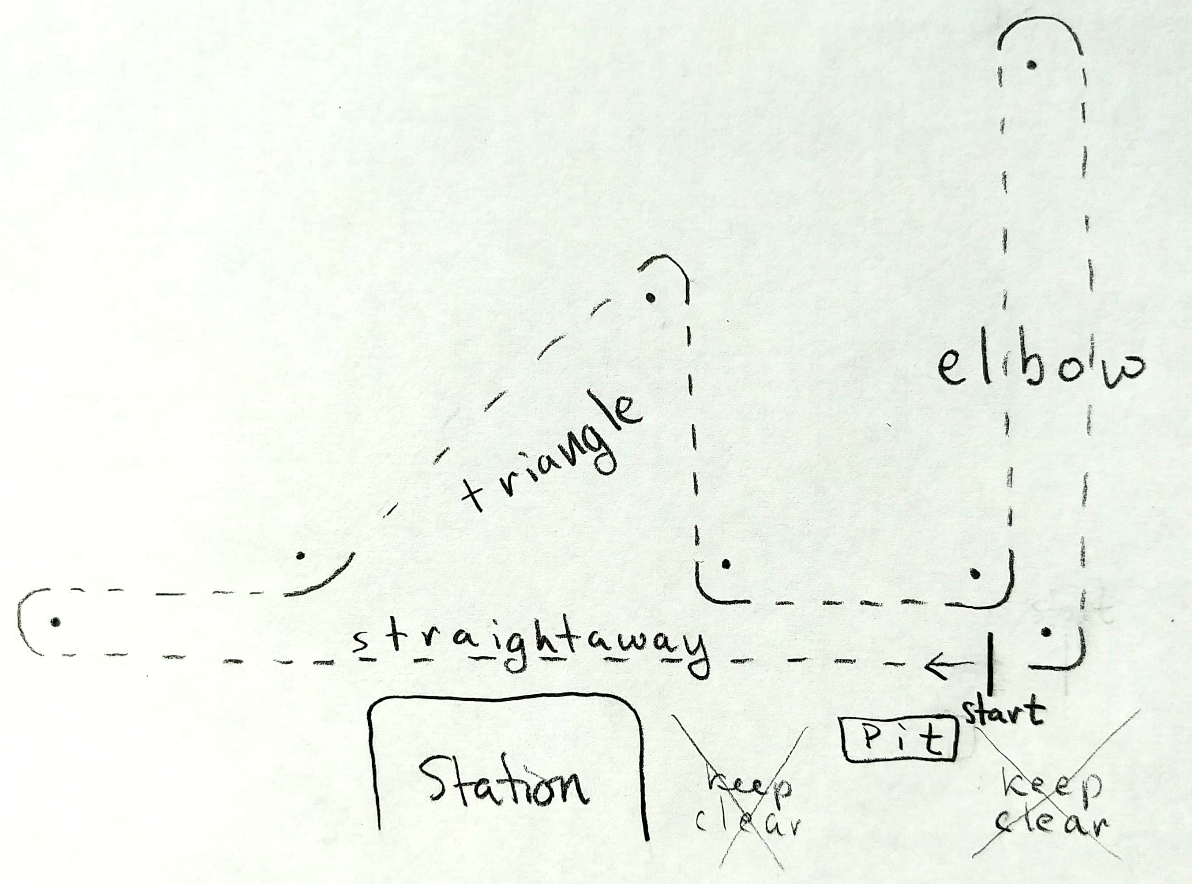
\includegraphics[scale=0.325]{Racetrack}

Then the race begins. Five laps with a pitstop after the third lap. The racetrack consists of a long straightaway mostly visible to the crowd, a triangular maneuvering section fully visible, and an elbow section only visible on TV.

\begin{tabular}[t]{| c | p{12.5cm} |}
\toprule
\multicolumn{2}{|l|}{Table \ref{quest_4}.1 Problems on the Straightaway} \\
\midrule
1d4 & Problem \\
\midrule
1 & Engine pushed too hard. \newline \qtwo{The engine's vent is overheating, pushing the radiator to its limit and potentially warping the exhaust vent.}{The engine's fuel flow starts to sputter as it fails to keep up with demand.} \\
2 & Such acceleration knocks a piece of hull off. The pilot has to considerably adjust their burns to account for the changed center of mass. \\
3 & Such acceleration ends up locking the controls in place. The pilot has to either yank extremely hard or completely stop accelerating before they're able to turn. \\
4 & No problem occurs. \\
\bottomrule
\end{tabular}

\vspace{0.2cm}
\begin{tabular}[t]{| c | p{12.5cm} |}
\toprule
\multicolumn{2}{|l|}{Table \ref{quest_4}.2 Problems in the Triangle} \\
\midrule
1d4 & Problem \\
\midrule
1 & The sweeps of the triangle require very precise control of the nose cone. The fighter uses electric gyroscopes to position this, which may become demanding on the reactor. The pilot may have to manually turn the nose cone or end up traveling in the wrong direction. \\
2 & The constant stopping and starting of the engine eventually leads to an ignition failure. The engine requires several ingitions to ignite rather than one, which can delay a burn enough to knock the pilot significantly off course. \\
3 & The exhaust steam of a ship ahead gets in the way of the pilot's vision. The pilot has to guess when to initiate the turn, since the computer guidance is based on visual and infrared input as well. \\
4 & No problem occurs. \\
\bottomrule
\end{tabular}

\vspace{0.2cm}
\begin{tabular}[t]{| c | p{12.5cm} |}
\toprule
\multicolumn{2}{|l|}{Table \ref{quest_4}.3 Problems around the Elbow} \\
\midrule
1d4 & Problem \\
\midrule
1 & The brazier racer launches fireworks directly at broadcasting cameras as well as in the faces of every other racer. \\
2 & The glacier racer "accidentally" shatters some shards of ice directly in the path of the racers behind them. \\
3 & Allow the players to try a strategy of their own. If they're just winging it, give them a chance to accelerate forward and become the race leader. \\ 
4 & No problem occurs. x``\\
\bottomrule
\end{tabular}

\vspace{0.2cm}
\begin{tabular}[t]{| c | p{12.5cm} |}
\toprule
\multicolumn{2}{|l|}{Table \ref{quest_4}.4 Problems during the Pitstop} \\
\midrule
1d8 & Roll at least two different problems. \\
\midrule
1 & A piece of metal in the fighter is warped enough to destabilize the craft. \\
2 & An electric wire somewhere in the ship is fried and needs replacement. \\ 
3 & A seal keeping in the fuel is leaking. \\ 
4 & Noticeable excess radiation is detected. \\
5 & A seal keeping in the thermal fluid is leaking. \\ 
6 & The pilot's window is cracked. \\
7 & One of the RCS jets that allows the fighter to control its orientation is blocked by debris. The debris is small but frozen on, stopping a valve from opening. \\
8 & The ignition sparker is gunked up with random poorly-combusted exhaust and other debris. \\
\bottomrule
\end{tabular}


\newpage
\section{Documentation}

The following few subsections include a justification for the ship weaponry used. They are written in denser language and are not necessary to run the campaign.

\subsection{To Hit a Fighter}

Consider a situation where a fighter ship wants to dodge a railgun shot fired at it. The railgun's cameras and targeting systems are so advanced that the fighter's position, velocity, and acceleration are known. 

The fighter cannot do anything to dodge before the shot is fired. If the fighter tries to dodge before, its velocity will change. However, the targeting systems know the fighter's velocity, so any change in velocity can be accounted for by aiming the railgun. Any acceleration taking place at the moment the shot is fired is also taken into account. Therefore the fighter must accelerate after the shot is fired in order to dodge it.

Since velocity and acceleration are accounted for, the only velocity and acceleration that matter are those that are gained after the shot is fired. The fighter then must accelerate a sufficient amount after the shot is fired in order to dodge it. During this acceleration, where the initial velocity and acceleration are accounted for and therefore can be treated as zero, the total distance traveled $d$ over a time $t$ is given by 

\begin{equation} d = \frac{1}{2}at^2 \end{equation}

where $a$ is the acceleration, assuming it is held roughly constant. The total distance needed to be traveled in order to dodge a shot aimed at the center of a ship is half of the length of the ship. Since the engine is positioned only at the back of the ship, this length is strictly along the forward-backward axis of the fighter. Using $ d = \frac{1}{2} l $ and solving for time, the equation above becomes
\begin{equation} \label{dodge_time}
t = \sqrt{\frac{l}{a}}
\end{equation}
This equation takes the ship's length $l$ and maximum acceleration $a$ and yields a time $t$ which represents how long it takes the ship to accelerate over half of its length. If a shot takes less than this amount of time to arrive, the ship will not have enough time to accelerate over half of its length, meaning the shot will hit the ship somewhere. If a shot takes more than this amount of time to arrive, the ship will have enough time to dodge over half of its length, and so the shot will not hit. This \textit{dodge time} is an effective measure of a fighter's ability to maneuver. 

The dodge time can also be converted into a range. If a railgun fires a shot at initial velocity $v$, then the distance it travels in a certain amount of time $t$ is 

\begin{equation} d = vt \end{equation}

Using the proof above that the shot must take less than the dodge time \ref{dodge_time} to arrive or else it will always miss a fighter that dodges it, the equation above becomes 
\begin{equation} \label{effective_range}
d = v \sqrt{\frac{l}{a}}
\end{equation}
This equation gives the \textit{effective distance} $d$ that a railgun can fire at a specific fighter. If the railgun fires at a fighter past this distance, the shot's speed will be too slow to cover the distance within the time required by the fighter's dodge time. This equation can help a savvy DM determine exactly whether or not a Gunner or Pilot can hit a small enemy ship at a given range, assuming they are going to dodge it. If the enemy does not dodge, the actual range of the weapon can be longer.

To recap, the proper measure of a fighter's defense against railguns is its \textit{dodge time} found in equation \ref{dodge_time}. A railgun's \textit{effective range} found in equation \ref{effective_range} will depend on the ship it is firing at. A railgun that fires faster typically has longer ranges.

\subsection{Weapon Accuracy}

Consider a weapon firing a shot at a target ship. The weapon aims at a single point, and the perfect straight line between the weapon and that point is the original trajectory of the shot. Call this distance $R$. However, every shot inevitably leaves the muzzle with some error in angle $\delta \theta$ that causes the real trajectory to deviate from the original. 

The shot arrives at the target. A right triangle is formed between the muzzle of the weapon, the point on the target the weapon was aimed at, and the real point that the shot arrives at. 

\begin{minipage}[t]{\linewidth} \centering
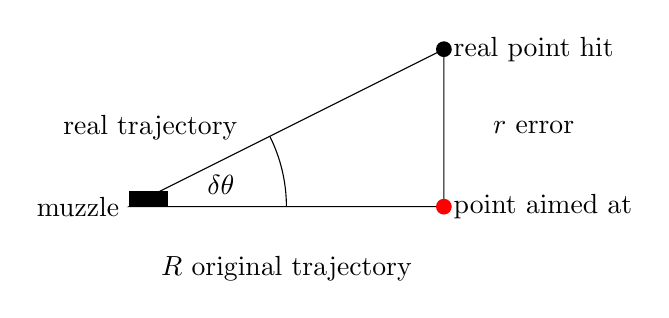
\begin{tikzpicture}
\coordinate (M) at (0, 0);
\coordinate (A) at (4, 0);
\coordinate (E) at (4, 2);

\draw (A) node[anchor=west]{point aimed at} 
-- (M) node[anchor=east]{muzzle} 
-- (E) node[anchor=west]{real point hit} 
-- cycle
pic [draw=black, angle radius=2cm, "$\delta\theta$"] {angle= A--M--E};

\fill [black] (M) rectangle (0.5, 0.2);
\fill [red] (A) circle (0.1);
\fill [black] (E) circle (0.1);

\draw (2, -0.5) node[anchor=north]{$R$ original trajectory};
\draw (4.5, 1) node[anchor=west]{$r$ error};
\draw (1.5, 1) node[anchor=east]{real trajectory};
\end{tikzpicture}
\end{minipage}

Using a tangent the following relation can be derived from the above triangle

\begin{equation} tan(\delta\theta) = \frac{r}{R} \end{equation}

Assume that the length of the original trajectory is significantly larger than the length of $r$ the error. That is, $ R >> r $. This ensures that $\delta\theta$ is a very small number, so that the small angle approximation $tan(x) = x$ can be used to simplify the equation above into

\begin{equation} \delta\theta = \frac{r}{R} \end{equation}

Rearranging,

\begin{equation} \label{accuracy}
r = R \delta\theta
\end{equation}

is an equation that tells the maximum possible error $r$ in the arrival of the shot at the target, over a distance $R$ and assuming a maximum error in angle of $\delta\theta$.

A shot aimed at the center of a target must ensure that $r$ never becomes larger than half of the length of the smallest dimension of the target. More than this and the shot might miss the target, solely due to the inherent error in angle as the shot leaves the muzzle. This equation is applicable to any kind of weapon that fires a shot at a specific point, including railguns, rays, and lasers. A savvy DM could use this equation to determine whether or not a Gunner or Pilot can reliably hit a specific part of a large ship or station at a given range. 

\subsubsection{Putting Numbers To It}

Both railguns and rays can use magnets at the end of the barrel to finely target the weaponry. This kind of targeting is similarly used by CRT televisions. How far away could a railgun or ray shoot at a fighter ship and reliably hit, assuming the same accuracy as an old CRT television?

A CRT television measures approximately 100cm along the diagonal and 80 cm deep. This results in full dimensions of approximately 60x80x80cm. The standard resolution at the time was 449x483 pixels at 4:3 ratio. Dividing each dimension of the screen by the number of pixels results in the smallest dimension of a single pixel being $2r=$0.134cm. The depth is $R=$80cm. Using equation \ref{accuracy} results in $\delta\theta=$2.87 arc minutes (or 8.35$*10^-4$ radians).

Consider a railgun attempting to hit a target. The target's smallest dimension is about 4m resulting in $r=$2m. Assume the same accuracy as a CRT television, $\delta\theta=$2.87 arc minutes. Using equation \ref{accuracy} results in $R=2390$m. A railgun or ray can reliably hit a fighter-sized target within around 2500m. This assumes only accuracy considerations, so the fighter is stationary and does not dodge. Any reasonably player should accept that a military-grade weapon is 4 or more times as accurate as an old 1950s-era CRT television set, meaning your battlefields can be on the scale of 10000m or 10km. A target at twice the distance of $R=2390$m would be hit by the railgun or ray only a quarter as often, rather than only half as often. This means that this distance is a cutoff that rapidly drops off.


\subsection{On Laser and Missile Weaponry}

\subsubsection{Lasers}

Consider a laser weapon being fired at a target. In order to properly heat up a target, the laser must be fired at exactly the same place for long amounts of time.

The laser hits the shot at an initial point. The energy transferred is spread over an area based on the radius of the laser beam. This area is a perfect circle. If the laser wants to maintain proper heating of that initial point, the laser can drift by no farther than the radius of the initial area. Farther than that and no heat will transfer from the laser to the initial point. 

We can treat this situation as an accuracy problem described in the section above. The error $r$ must be no larger than the radius of the laser $r_\text{laser}$ as it arrives. This value can be approximated as the initial radius of the laser, though the final radius will be larger. So approximate $r~=$40cm \cite{strong_laser}. The distance the laser is shooting from is $R$. The error in angle of firing the laser is $\delta\theta$. So equation \ref{accuracy} holds and returns an effective range for a laser weapon to be $R~=478$m. A laser effectively has to hit its own shot every second, and the laser beam is smaller than the target, meaning a laser always has considerably less range than a railgun or ray.

\subsubsection{Missiles}

Missile weaponry are more simple to debunk. The missiles are simply shot out of the sky before they can do anything. Treat a missile like a fighter so that equation \ref{effective_range} applies to it. A railgun firing at a modest $v=$3km/s at a missile of length $l=$4m which can accelerate at ten times the maximum of a human being $a=$100g$=$980.6m/s$^2$. These values result in an effective range for a railgun against the missile of 192m, assuming the missile constantly chooses new directions to accelerate at full speed.

While a missile may not be able to hit a missile in time, a ray certainly will. The missile's length was conservatively 4m, while its width is $2r=$1m, approximating. Applying equation \ref{accuracy} with the standard 2.87 arc minutes of accuracy yields a range of $R=$599m. Both railguns and rays can hit the railgun before it arrives, and rays can hit it reliably quite before it arrives. Considering that a single hit from a railgun or ray can instantly disable a hugely-expensive missile, missiles are not used often during combat.



\newpage
\begin{thebibliography}{8} % ALWAYS UPDATE THIS NUMBER WHEN ADDING
\bibitem{naval_railgun} 
Adams, D. A. (2003). Naval rail guns are revolutionary. \textit{US Naval Institute}. Retrieved from \url{https://web.archive.org/web/20070708054858/http://edusworld.org/ew/ficheros/2004/railguns.pdf}

\bibitem{energy_weapons}
Bloembergen, N., Patel, C. K. N., et al. (1987). Report to the American Physical Society of the study group on science and technology of directed energy weapons. \textit{Reviews of Modern Physics} 59, 3 II. \url{https://doi.org/10.1103/RevModPhys.59.S1}

\bibitem{recycling_water_and_air} 
Closing the Loop: Recycling Water and Air in Space [PDF file]. (n.d.). Summary of inaccessible video. \textit{NASA}. Retrieved from \url{https://www.nasa.gov/pdf/146558main_RecyclingEDA(final) 4_10_06.pdf}

\bibitem{strong_laser}
Ivanov, N., Losev, V., Panchenko, Y., and Tarasenko, V. (2017). High-power laser systems of UV and visible spectra ranges. \textit{IntechOpen}. \url{https://doi.org/10.5772/intechopen.71455}

\bibitem{kevlar_properties}
Kevlar Aramid Fiber Technical Guide [PDF file] (2017). \textit{DuPont}. Retrieved 9 November 2019. Retrieved from \url{http://www.dupont.com/content/dam/dupont/products-and-services/fabrics-fibers-and-nonwovens/fibers/documents/Kevlar_Technical_Guide_0319.pdf}

\bibitem{scientific_railgun}
Rashleigh, S. C. and Marshall, R. A. (1978). Electromagnetic acceleration of macroparticles to high velocities. \textit{Journal of Applied Physics} 49, 2540. \url{https://doi.org/10.1063/1.325107}	

\bibitem{international_temperature_scale_of_1968} 
Rossini, F. D. (1968). A Report on the International Temperature Scale of 1968. Retrieved from \url{http://media.iupac.org/publications/pac/1970/pdf/2203x0555.pdf}

\bibitem{hydrogen_recapture} 
Shah, N., Panjala, D., and Huffman, G. P. (2001). Hydrogen production by catalytic decomposition of methane. \textit{Energy Fuels} 15, 6, 1528-1534. \url{https://doi.org/10.1021/ef0101964}
\end{thebibliography}
\end{document}
